\chapter{Calibration Hardware for Dual-Phase}
\label{ch:dp-calib}

%%%%%%%%%%%%%%%%%%%%%%%%%%%%%%%%%%%%%%%%%%%%%%%%%%%%%%%


\section{Introduction}
\label{sec:dp-calib-ov}


This chapter focuses on describing the dedicated calibration hardware systems deployed for the \dword{dune} \dword{dp} \dword{fd} module and providing necessary information beyond the reach of external measurements and existing sources and monitors. These include an ionization laser system, a photoelectron laser system, 
and a \dword{pns} system. A possible radioactive source system is also being explored. The responsibility for the calibration hardware systems fall under the joint \dword{sp} and \dword{dp} calibration consortium formed in November 2018.

A detailed understanding of the overall detector response is essential for \dword{dune} physics goals. Each calibration parameter must be measured precisely according to the requirements on the %JM
systematic uncertainties for the \dword{lbl}, low-energy (\dword{snb}), and other physics programs at \dword{dune}. The calibration 
program 
%plan %JM;
must provide stable measurements at a few-percent-or-better 
%few-percent %JM; SG: this was a language edit from editors
level across an enormous volume and over a long period while providing sufficient redundancy. The physics volume of the \dword{tdr} provides a detailed description of the calibration strategy for the \dword{dune} \dword{fd}; here, we provide a brief summary.

The current calibration strategy for \dword{dune} uses existing sources of particles, external measurements, and dedicated external calibration hardware systems. Existing calibration sources for \dword{dune} include beam or atmospheric neutrino-induced samples, cosmic rays, argon isotopes, and instrumentation devices such as \dword{lar} purity and temperature monitors. Dedicated calibration hardware systems comprise laser and neutron source deployment systems.  External measurements by \dword{protodune} and \dword{snb} experiments  will validate techniques, tools, and design of systems for the \dword{dune} calibration program. These sources and systems measure detector response model parameters or provide tests of the response model itself. Calibration measurements can also correct data, data-driven efficiencies, systematics, and particle responses.

%Chapter~4 of the Physics volume of the \dword{tdr} provides a more detailed description of the calibration strategy for the \dword{dune} \dword{fd}. 
%using existing sources of particles (e.g., cosmic ray muons), external measurements (e.g., \dword{protodune}), monitors (e.g., purity monitors), and dedicated calibration hardware systems. 


%This chapter describes the design of the dedicated calibration systems to be deployed for the DUNE \spmod.  As discussed in the Physics TDR\fixme{proper reference}, the calibration strategy includes external measurements (e.g. ProtoDUNE), monitors (e.g. purity, thermal), existing sources of particles (e.g. muons from cosmic rays), and dedicated external calibration hardware systems.  This chapter discusses the calibration hardware systems. Monitoring systems are discussed in other chapters: CISC (purity, thermal monitors, slow control), PDS (LED stability system\fixme{proper name is?}), and CE (charge injection system). The physics TDR discusses the use of existing sources of particles, and external measurements. 

Calibration systems are used at each stage of the experiment. Once the \dword{fd} is filled and at the desired high voltage, it immediately becomes live for 
non-beam physics
%\dword{snb} and proton decay signals (beam and atmospheric neutrino physics will require a few years of data accumulation) 
at which point  %for %JM
early calibration must track %to track %JM
the space-time dependence of the detector. Dedicated early calibration runs using calibration hardware systems develop and tune calibration tools to beam data taking and correct for any space-time irregularities observed in the \dword{tpc}. Given the expected low rate of cosmic ray events at the underground location, calibration using cosmic rays is not possible over short time scales and will proceed from coarse-grained to fine-grained over the course of years, as statistics accumulate. 
The experiment will rely on calibration hardware systems, such as a laser system, for calibrations that require an independent probe with reduced or removed interdependencies, fine-grained measurements (both in space and time), and detector stability monitoring on the time scales required by physics. Calibration systems such as a neutron source system provide low-energy electromagnetic response at the precision required for low-energy \dword{snb} physics. 
Once the detector is running stably, dedicated calibration runs (ideally before, during, and after each run period) will ensure that detector conditions have not changed significantly. As \dword{dune} becomes systematics-limited, dedicated precision-calibration campaigns using the calibration hardware systems must help meet the stringent physics requirements on energy scale reconstruction and detector resolution.

%Section~\ref{sec:sp-calib-ov-scope} describes the baseline calibration hardware designs. 
%and outlines alternative designs that may improve the physics capability and/or reduce overall cost. 
Section~\ref{sec:dp-calib-sys} describes the baseline calibration hardware designs. Section~\ref{sec:dp-calib-sys-las-ion} describes the baseline design for the ionization laser system that provides an independent, fine-grained measurement of the electric field throughout the detector, an essential parameter that affects the spatial and energy resolution of physics signals. The \dword{dune} \dword{cdr}~\cite{Acciarri:2015uup} assumes that the \dword{fv} is known to the \SI{1}{\%} level. By measuring spatial distortions and drift velocity map, the laser calibration system also 
%mainly 
helps define the detector \dword{fv}, thus allowing correct predictions of the \dword{fd} spectra. The laser system also offers many secondary uses such as alignment checks, stability monitoring, and diagnosing detector performance issues. 
%Alternative designs for the ionization laser system that may improve the physics capability and/or reduce overall cost are also under development and are described in Appendix~\ref{sec:sp-calib-laser-alter}.
Section~\ref{sec:dp-calib-sys-las-pe} describes the photoelectron laser system that can be used to rapidly diagnose electronics or \dword{tpc} response issues along with many other useful measurements such as integrated field across drift, drift velocity, and electronics gain. 

Section~\ref{sec:dp-calib-sys-pns} describes the baseline design for the \dword{pns} system, which provides a triggered, well defined energy deposition from neutron capture in Ar detectable throughout the detector volume. Neutron capture is a critical component of signal processes for \dword{snb} and \dword{lbl} physics, enabling direct testing of the detector response spatially and temporally for the low-energy program and the efficiency of the detector in reconstructing the low-energy spectra. The proposed \dword{rsds}, which is in many ways complementary to the \dword{pns} system, can provide at known locations inside the detector a source of gamma rays in the same energy range of \dword{snb} and solar neutrino physics. The \dword{rsds} is the only calibration system that can probe detection capability for single isolated solar neutrino events and study how well radiological backgrounds can be suppressed. In contrast, the \dword{pns} is externally triggered and does not provide such a well-defined source location for gamma rays inside the detector, but on the other hand, the \dword{pns} can probe the uniformity of the full detector. The \dword{rsds} can only scan the ends of the detector in the proposed deployment scheme. The proposed complementary \dword{rsds} system is described in the Appendix~\ref{sec:dp-calib-sys-rsds}. 

For all the calibration hardware systems, the goal is to deploy prototype designs and validate them in \dword{protodune} as part of the post long shutdown 2 (LS2) running  at \dword{cern}. The validation plan for calibration systems at \dword{protodune} and other experiments is described in Section~\ref{sec:dp-calib-val}. The \dword{daq} requirements for calibration systems are described in Section~\ref{sec:dp-calib-daqreq}. The schedule and milestones for calibration systems is discussed in Section~\ref{sec:dp-calib-sched}.

%The calibration consortium was formed in November 2018. Significant development plans exist, and their timeline is in Section~\ref{sec:sp-calib-sched}.
%A large part of the work done so far has been done within the Calibration Task Force; 

%%%%%%%%%%%%%%%%%%%%%%%%%%%%
\subsection{Scope}
\label{sec:dp-calib-ov-scope}
% KM outline
%% Scope is: baseline designs for Laser system and neutron system.
%% Alternative designs, including additional capabilities of the laser system, radioactive source are considered.

%%calibration review in May. "what's the scope? How many lasers we need? How many ports needed? Do we need crossing tracks? do we need to penetrate FC ? what does the HV consortium think about that?"

The scope of the calibration consortium includes a laser ionization system, a laser photoelectron laser system, a laser positioning system, and a \dword{pns} system. In addition, the consortium is evaluating a \dword{rsds}. The calibration consortium is responsible for overall design through commissioning in the \dword{dp} module for these calibration devices and their associated feedthroughs. Validating the designs of calibration systems at \dword{protodune} (and other relevant experiments) is also included under the scope of the consortium. Figure~\ref{fig:calib_scope_chart} shows the subsystems included under the calibration consortium. 

Chapter 2 describes other hardware essential for calibration such as the \dword{crp} charge injection pulsing system, Chapter 4 the
%\dword{ce} external charge injection systems, 
\dword{hv} monitoring devices, Chapter 5 the \dword{pds} stability monitoring system, and Chapter 7 the cryogenic instrumentation and detector monitoring devices. \fixme{Should these chapters have a LATEX code for location?} The scope of these systems are described by their respective consortia, and the calibration consortium has substantial interfaces with these consortia. 

The use of other calibration sources such as external measurements and existing sources of particles (e.g., muons, pions) is discussed in the physics volume of the \dword{tdr} \fixme{Again, does the location in LATEX need to be included?}. The calibration task force is pursuing the effects of calibration on physics and related studies, and the consortium works closely with the task force to make physics connections. Calibrations also require simulations (e.g., \efield) to identify desirable locations for calibration devices in the cryostat, away from regions of high \efield, so their presence does not induce large field distortions. 
%Calibration has additional activities outside the scope of the consortium that require coordination with other groups. This is discussed in Section~\ref{sec:sp-calib-intfc}. 
The design of the calibration systems and understanding the related physics requires coordinating with other consortia and groups. This is discussed in Section~\ref{sec:dp-calib-intfc}.
%, which also includes necessary tools (e.g., physics simulations) developed in conjunction with the physics groups and calibration task force.

%\fixme{Please use dunefigures! Here's a template (the label should be fig:filename):}

%\begin{dunefigure}[short caption]{label}
%{long caption}
%\includegraphics[width=0.8\textwidth]{filename}
%\end{dunefigure}

%\begin{figure}[tbp]
%\centering
%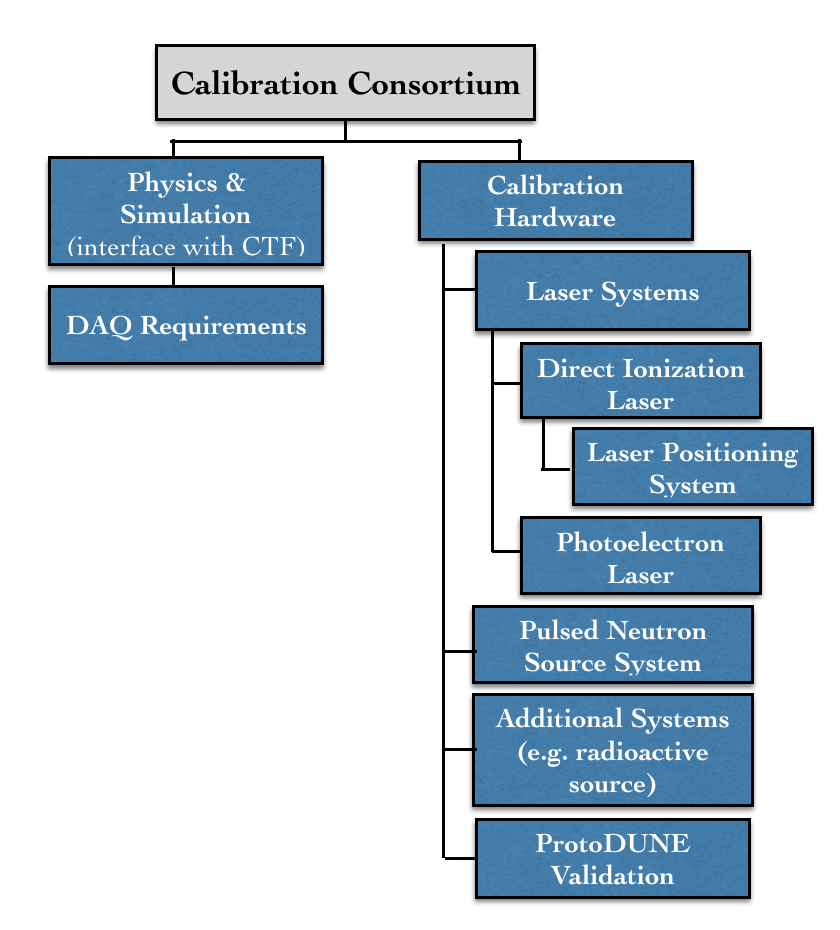
\includegraphics[height=4.0in]{graphics/calib_scope_chart.png}
%\caption{Calibration consortium subsystem chart.}
%\label{fig:scope_chart}
%\end{figure}

\begin{dunefigure}[Calibration consortium subsystem chart]{fig:calib_scope_chart}
{Calibration consortium subsystem chart.}
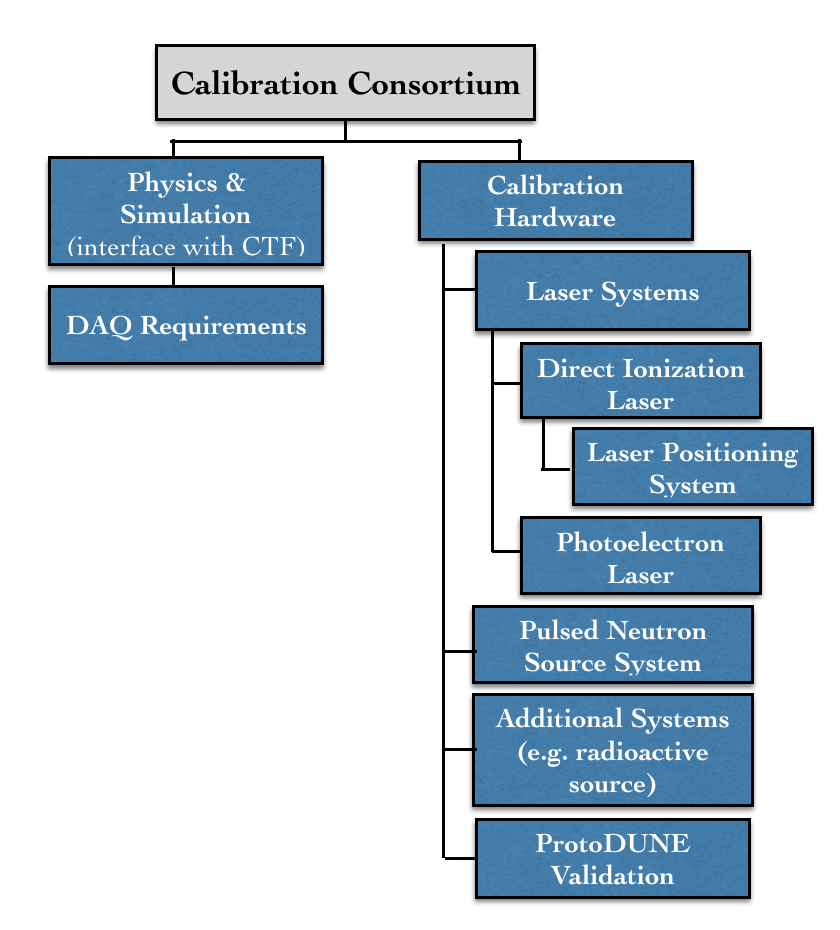
\includegraphics[height=4.0in]{graphics/calib_scope_chart.png}
\end{dunefigure}

%%%%%%%%%%%%%%%%%%%%%%%%%%%%
%\subsection{Requirements}
%\label{sec:sp-calib-ov-req}

%\input{vol-sp/ch-dp-calib-requirements}


%%%%%%%%%%%%%%%%%%%%%%%%%%%%
\subsection{Design Considerations and Requirements}
\label{sec:dp-calib-ov-consid}
%\fixme{SG, KM: Done; JM please check. }
%To-DO: Need more information on requirements from neutron source and RA source, once we have it, we can update the text/table as needed.}
%\fixme{SG/JM done; need to put in autogenerated requirements table; Anne et al., working on it}
Some common design considerations for calibration devices include stability, reliability, and longevity, so calibration systems can be operated for the lifetime of the experiment (\dunelifetime). Such longevity is uncommon for any device, so the overall design permits replacing devices where possible. The systems must also adhere to relevant global requirements of the \dword{dune} detector. Table~\ref{tab:specs:DP-CALIB} shows the top-level overall requirements for calibration subsystems. For example, \dword{dune} requires the \efield on any instrumentation devices inside the cryostat to be less than 30 kV/cm to minimize the risk of dielectric breakdown in \dword{lar}. Another consideration important for reconstructing events is the maximum noise level the readout electronics can tolerate from calibration devices. 
%\fixme{is the following sentence true for DP too? We need to either change it or remove it. SG: yes, PDDP is evaluating this.}
We are evaluating this using \dword{pddp}. 

Developing the \dword{sp} module calibration systems has already started, so the design considerations for \dword{dp} closely follow \dword{sp} while taking into account some important differences.

The longer drift length of \dpmaxdrift in \dword{dp} (instead of \spmaxdrift in \dword{sp}) suggests that diffusion causes a wider spread in the size of the electron cloud. For the nominal field of \dpnominaldriftfield, the transverse diffusion coefficient is \SI{13.1586}{\square \cm \per \s} \cite{Li:2015rqa,larpropertiesbnl}, leading
%% calculation sigma = sqrt(2*D_T*t) where t = L/v s the drift time
%% v = 0.1648 cm/us = 0.1648e6 cm/s
%% sqrt(2*13.1586*1200/(0.1648e6)) 
to a maximum spread of \SI{4.4}{\milli\m}; the maximum in \dword{sp}, for a \spmaxdrift drift, is \SI{2.4}{\milli\m}. Taking these values in quadrature with the readout pitch, which is smaller in \dword{dp}, the spatial precision is about \SI{5.3}{\milli\m}, comparable in both detectors. 

The longer drift length in \dword{dp} leads to proportionally higher ion charge accumulation and higher space charge effects. This is compounded by the fact that the charge multiplication in the gas phase leads to ion feedback into the liquid. We therefore expect larger \efield distortions in \dword{dp}, up to about \SI{15}{\%}~\cite{bib:boyu2018}.
%\fixme{JM: the next sentence, might be a bit too obvious, so I commented out to avoid a lengthy intro.}
However, the relative effect of a \SI{1}{\%} distortion of the \efield in the liquid phase on the amount of charge reaching the gas-liquid interface should be similar to the effect of a \SI{1}{\%} distortion of the \efield in the \dword{sp} on the amount of charge reaching the \dword{apa} wires. Therefore, in terms of energy response, the requirements on \efield measurement precision should be similar in both \dword{sp} and \dword{dp}.

%\paragraph{Laser system}
%{\bf Laser System:} 
For the laser system, the energy and position reconstruction requirements for physics measurements lead to requirements for precision in measuring the laser \efield as well as its spatial coverage and granularity. 
 The laser \efield measurement precision must be approximately \SI{1}{\%}, so the effect on the collected charge is well below \SI{1}{\%}. This is also motivated by consistency with the high level \dword{dune} specification of \SI{1}{\%} on field uniformity throughout the volume for component alignment and the \hv system. For laser coverage, to keep the overall \efield measurement at the $\sim$\SI{1}{\%} level, even with possible large distortions in the unmeasured region, the specification requires coverage of \SI{93}{\%} or more of the total \dword{fv}. This is more than in \dword{sp} because the maximum expected distortions are also larger. 
 The granularity requirement for the laser measurement is estimated based on the \dword{fv} uncertainty requirements (\SI{1}{\%}) and corresponding uncertainty requirements (\SI{1.5}{\cm}) in each coordinate. The required voxel size will depend on the magnitude of the \efield distortions. In regions of large distortions (of up to \SI{15}{\%}, which is possible because of gas phase ion feedback), \num{10}$\times$\num{10}$\times$\SI{10}{\cubic\cm} granularity is necessary, but  \num{30}$\times$\num{30}$\times$\SI{30}{\cubic\cm} should be sufficient for distortions up to \SI{5}{\%}, as discussed in Section~\ref{sec:dp-calib-laser-req}

The laser beam position must also meet the level of reconstruction requirement in each coordinate, approximately \SI{5}{\milli\m} over \SI{15}{\m}, where the latter is the distance between two consecutive laser ports in the beam direction. This results in a stringent requirement of \ang{0.03} (or \SI{0.5}{\mrad}). In terms of design constraints, the absence of detector elements (like \dwords{apa} and \dwords{cpa} in \dword{sp}) within the \dword{tpc} makes it easier to cover the \dword{dp} module with fewer beams, as long as \dword{fc} penetration is possible. 
%\fixme{JM: We already talk about this in the Interface section. Maybe we don't need to repeat here? I'm OK with commenting these next 2 sentences out. SG: agreed.}
%Interfaces with the \dword{pds} need careful evaluation, since it will not be possible to avoid hitting the reflector panels. The PMTs' HV will likely need to be turned off for the laser calibration. 

%The data volume for the ionization laser system must be at least \num{90}~TB/year/\SI{10}{\kt}, assuming \num{800}k laser pulses, \num{10}$\times$\num{10}$\times$\SI{10}{\cubic\cm} voxel sizes, a \SI{100}{\micro\s} zero suppression window, and one dedicated calibration campaign per year.\todo{Need to update DAQ calculation based on number of channels.}

The data volume for the ionization laser system must be at least \num{20}~TB/year/\SI{10}{\kt}, assuming \num{400}k laser pulses, \num{10}$\times$\num{10}$\times$\SI{10}{\cubic\cm} voxel sizes, a \SI{100}{\micro\s} zero suppression window, and one dedicated calibration campaign per year.

%\paragraph{\dlong{pns}}
%{\bf \dlong{pns}:} 
For the \dword{pns} system, fewer detector elements leads to a more uniform distribution of neutrons, an advantage of \dword{dp}. On the other hand, if injected from the top, the neutrons must penetrate the readout planes, which can reduce the neutron flux going into the argon. This is currently under investigation. For the \dword{pns} system, the system must provide a sufficient neutron event rate to make spatially separated precision measurements across the detector of a comparable size to the voxels probed by the laser (\num{30}$\times$\num{30}$\times$\SI{30}{\cubic\cm}) for most regions of the detector (\SI{75}{\%}). 
% 1st draft
%For the supernova program, measurements from the \dword{pns} \fixme{This abbreviation is in neither glossary.} should demonstrate 1\% energy scale, 5\% energy resolution, and 0.5 MeV detection threshold, so each voxel should have sufficient neutron event rate to achieve this. %\todo{KM: Improve or remind connection to SN program? even though it's comparable? SG: maybe for 2nd draft?}
%rewritten for 2nd draft
For the supernova program, the sensitivity to distortions of the neutrino energy spectrum depends on the uncertainties in the detection threshold and the reconstructed energy scale and resolution. Studies discussed in the physics \dword{tdr} \fixme{Does this require a LATEX location code?} present target ranges for the uncertainties in these parameters as a function of energy. The measurements with the \dword{pns} should provide response corrections and performance estimates, so those uncertainty targets are met throughout the whole volume, and so each voxel has a sufficient neutron event rate (percent level statistical uncertainty).

%\fixme{Insert correct reference to physics TDR ch7}
%\fixme{Put PNS in glossary and use that.}
In terms of data volume requirements, the \dword{pns} system needs approximately \num{100}~TB/year/\SI{10}{\kt}, assuming \num{e6} neutrons/pulse, \num{1000} neutron captures/\si{\cubic\m}
%m$^{3}$ 
and \num{1300} observed neutron captures per pulse, and six calibration runs per year.
%\todo{Need to update DAQ calculation based on number of channels.} 

Table~\ref{tab:fdgen-calib-all-reqs} shows the full set of requirements related to all calibration subsystems. More details on each requirement can be found under dedicated subsections.   
%\todo{SP-CALIB-3 is coming out weird in table 1.1, needs to be fixed.}

%\fixme{Can the second part of this title be put in a footnote to Table 1.1? SG: we would prefer to leave it here}

%\fixme{Anne uncommented 5/20 (uncomment when spec table available)}
%%% This file is generated, any edits may be lost.

\begin{longtable}{p{0.14\textwidth}p{0.13\textwidth}p{0.18\textwidth}p{0.22\textwidth}p{0.20\textwidth}}
\caption{Specifications for DP-CALIB \fixmehl{ref \texttt{tab:spec:DP-CALIB}}} \\
  \rowcolor{dunesky}
       Label & Description  & Specification \newline (Goal) & Rationale & Validation \\  \colhline

   
  \newtag{DP-CALIB-1}{ spec:efield-calib-precision }  & Ionization laser \efield measurement precision  &  \SI{1}{\%} &  \efield affects energy and position measurements. &  ProtoDUNE and external experiments. \\ \colhline
     % 1
   \newtag{DP-CALIB-2}{ spec:efield-calib-coverage }  & Ionization laser \efield measurement coverage  &  $>\,\SI{93}{\%}$ \newline ( \SI{100}{\%} ) &  Allowable size of the uncovered detector regions is set by the highest reasonably expected field distortions, \SI{15}{\%}. &  ProtoDUNE \\ \colhline
     % 2
   \newtag{DP-CALIB-3}{ spec:efield-calib-granularity }  & Ionization laser \efield measurement  granularity  &  \SI{10 x 10 x 10}{\centi\metre} \newline ( \SI{10 x 10 x 10}{\centi\metre} ) &  Minimum measurable region is set by the maximum expected distortion and position reconstruction requirements. &  ProtoDUNE \\ \colhline
     % 3
   \newtag{DP-CALIB-4}{ spec:laser-position-precision }  & Laser beam position precision  &  \SI{0.5}{\milli\radian} \newline ( $<\,\SI{0.5}{\milli\radian}$ ) &  The necessary spatial precision does not need to be smaller than the CRP strip spacing. &  ProtoDUNE \\ \colhline
     % 4
   \newtag{DP-CALIB-5}{ spec:neutron-source-coverage }  & Neutron source coverage  &  $>\,\SI{75}{\%}$ \newline ( \SI{100}{\%} ) &  Set by the energy resolution requirements at low energy. &  Simulations \\ \colhline
     % 5
   \newtag{DP-CALIB-6}{ spec:data-volume-laser }  & Ionization laser DAQ rate per year (per 10 kt)  &  $>\,\SI{20}{TB/yr/10 kt}$ \newline ($>\,\SI{40}{TB/yr/10 kt}$) &  The laser data volume must allow the needed coverage and granularity. &  ProtoDUNE and simulations \\ \colhline
     % 6
   \newtag{DP-CALIB-7}{ spec:data-volume-pns }  & Neutron source DAQ rate per year (per 10 kt)  &  $>\,\SI{100}{TB/yr/10 kt}$ \newline ( $>\,\SI{200}{TB/yr/10 kt}$ ) &  The pulsed neutron system must allow the needed coverage and granularity. &  Simulations \\ \colhline
     % 7


\label{tab:specs:just:DP-CALIB}
\end{longtable}
% This file is generated, any edits may be lost.
\begin{footnotesize}
%\begin{longtable}{p{0.14\textwidth}p{0.13\textwidth}p{0.18\textwidth}p{0.22\textwidth}p{0.20\textwidth}}
\begin{longtable}{p{0.12\textwidth}p{0.18\textwidth}p{0.17\textwidth}p{0.25\textwidth}p{0.16\textwidth}}
\caption{Specifications for DP-CALIB \fixmehl{ref \texttt{tab:spec:DP-CALIB}}} \\
  \rowcolor{dunesky}
       Label & Description  & Specification \newline (Goal) & Rationale & Validation \\  \colhline

   \newtag{DP-FD-1}{ spec:dp-min-drift-field }  & Minimum drift field  &  $>$\,\SI{250}{V/cm} \newline ( $>\,\SI{500}{V/cm}$ ) &  Lessens impacts of $e^-$-Ar recombination, $e^-$ lifetime, $e^-$ diffusion and space charge. &  ProtoDUNE \\ \colhline
    
   
  \newtag{DP-FD-2}{ spec:dp-system-noise }  & System noise  &  $<\,\SI{1000}\,e^-$ &  Studies suggest that a minimum of 5:1 S/N on individual strip measurements allows for sufficient reconstruction performance. &  ProtoDUNE and simulation \\ \colhline
    
   \newtag{DP-FD-5}{ spec:lar-purity }  & Liquid argon purity  &  $<$\,\SI{100}{ppt} \newline ($<\,\SI{30}{ppt}$) &  Provides $>$5:1 S/N on induction planes for  pattern recognition and two-track separation. &  Purity monitors and cosmic ray tracks \\ \colhline
    
   
  \newtag{DP-FD-7}{ spec:dp-misalignment-field-uniformity }  & Drift field uniformity due to component alignment  &  $<\,1\,$\% throughout volume &  Maintains TPC and  FC orientation and shape. &  ProtoDUNE \\ \colhline
    
   
  \newtag{DP-FD-9}{ spec:dp-crp-strip-spacing }  & CRP strips spacing  &  $<\,\SI{4.7}{mm}$ &  Enables 100\% efficient MIP detection, \SI{1.5}{cm} $yz$ vertex resolution. &  Simulation \\ \colhline
    
   
  \newtag{DP-FD-11}{ spec:dp-hvs-field-uniformity }  & Drift field uniformity due to HVS  &  $<\,\SI{1}{\%}$ throughout volume &  High reconstruction efficiency. &  ProtoDUNE and simulation \\ \colhline
    
   \newtag{DP-FD-13}{ spec:dp-fe-peak-time }  & Front-end peaking time  &  \SI{1}{\micro\second} \newline ( Adjustable so as to see saturation in less than \SI{10}{\%} of beam-produced events ) &  Vertex resolution &   \\ \colhline
    
   
  \newtag{DP-FD-22}{ spec:dp-data-rate-to-tape }  & Data rate to tape  &  $<\,\SI{30}{PB/year}$ &  Cost.  Bandwidth. &  ProtoDUNE \\ \colhline
    
   
  \newtag{DP-FD-23}{ spec:dp-sn-trigger }  & Supernova trigger  &  $>\,\SI{95}{\%}$ efficiency for a SNB producing at least 60 interactions with a neutrino energy >10 MeV in 12 kt of active detector mass during the first 10 seconds of the burst. &  $>\,$90\% efficiency for SNB within 100 kpc &  Simulation and bench tests \\ \colhline
    
   
  \newtag{DP-FD-24}{ spec:dp-local-e-fields }  & Local electric fields  &  $<\,\SI{30}{kV/cm}$ &  Maximize live time; maintain high S/N. &  ProtoDUNE \\ \colhline
    
   
  \newtag{DP-FD-25}{ spec:de-non-fe-noise }  & Non-FE noise contributions  &  $<<\,\SI{1000}\,e^- $ &  High S/N for high reconstruction efficiency. &  Engineering calculation and ProtoDUNE \\ \colhline
    
   
  \newtag{DP-FD-26}{ spec:dp-lar-impurity-contrib }  & LAr impurity contributions from components  &  $<<\,\SI{30}{ppt} $ &  Maintain HV operating range for high live time fraction. &  ProtoDUNE \\ \colhline
    
   
  \newtag{DP-FD-27}{ spec:dp-radiopurity }  & Introduced radioactivity  &  less than that from $^{39}$Ar &  Maintain low radiological backgrounds for SNB searches. &  ProtoDUNE and assays during construction \\ \colhline
    
   \newtag{DP-FD-29}{ spec:dp-det-uptime }  & Detector uptime  &  $>\,$98\% \newline ($>\,$99\%) &  Meet physics goals in timely fashion. &  ProtoDUNE \\ \colhline
    
   \newtag{DP-FD-30}{ spec:dp-det-mod-uptime }  & Individual detector module uptime  &  $>\,$90\% \newline ($>\,$95\%) &  Meet physics goals in timely fashion. &  ProtoDUNE \\ \colhline
    

   
  \newtag{DP-CALIB-1}{ spec:efield-calib-precision }  & Ionization laser \efield measurement precision  &  \SI{1}{\%} &  \efield affects energy and position measurements. &  ProtoDUNE and external experiments. \\ \colhline
    
   \newtag{DP-CALIB-2}{ spec:efield-calib-coverage }  & Ionization laser \efield measurement coverage  &  $>\,\SI{93}{\%}$ \newline ( \SI{100}{\%} ) &  Allowable size of the uncovered detector regions is set by the highest reasonably expected field distortions, \SI{15}{\%}. &  ProtoDUNE \\ \colhline
    
   \newtag{DP-CALIB-3}{ spec:efield-calib-granularity }  & Ionization laser \efield measurement  granularity  &  \SI{10 x 10 x 10}{\centi\metre} \newline ( \SI{10 x 10 x 10}{\centi\metre} ) &  Minimum measurable region is set by the maximum expected distortion and position reconstruction requirements. &  ProtoDUNE \\ \colhline
    
   \newtag{DP-CALIB-4}{ spec:laser-position-precision }  & Laser beam position precision  &  \SI{0.5}{\milli\radian} \newline ( $<\,\SI{0.5}{\milli\radian}$ ) &  The necessary spatial precision does not need to be smaller than the CRP strip spacing. &  ProtoDUNE \\ \colhline
    
   \newtag{DP-CALIB-5}{ spec:neutron-source-coverage }  & Neutron source coverage  &  $>\,\SI{75}{\%}$ \newline ( \SI{100}{\%} ) &  Set by the energy resolution requirements at low energy. &  Simulations \\ \colhline
    
   \newtag{DP-CALIB-6}{ spec:data-volume-laser }  & Ionization laser DAQ rate per year (per 10 kt)  &  $>\,\SI{20}{TB/yr/10 kt}$ \newline ($>\,\SI{40}{TB/yr/10 kt}$) &  The laser data volume must allow the needed coverage and granularity. &  ProtoDUNE and simulations \\ \colhline
    
   \newtag{DP-CALIB-7}{ spec:data-volume-pns }  & Neutron source DAQ rate per year (per 10 kt)  &  $>\,\SI{100}{TB/yr/10 kt}$ \newline ( $>\,\SI{200}{TB/yr/10 kt}$ ) &  The pulsed neutron system must allow the needed coverage and granularity. &  Simulations \\ \colhline
    


\label{tab:specs:DP-CALIB}
\end{longtable}
\end{footnotesize}

%Full requirements table (not autogenerated) is below for completeness.
\begin{dunetable}
[Full specifications for calibration subsystems]
{p{0.45\linewidth}p{0.25\linewidth}p{0.25\linewidth}}
{tab:fdgen-calib-all-reqs}
{Full list of Specifications for the Calibration Subsystems.}   
Quantity/Parameter	& Specification	& Goal		 \\ \toprowrule      

Noise from calibration devices	 & $\ll$ 1000 enc   & \\ \colhline    Max. \efield near calibration devices & < 30 kV/cm & <15 kV/cm \\ \colhline                     

\textbf{Direct Ionization Laser System} &    &   \\ \colhline   
\efield measurement precision & 1\% & <1\% \\ \colhline
\efield measurement coverage & > 93\% & 100\% \\ \colhline
\efield measurement granularity & < \num{10}$\times$\num{10}$\times$\SI{10}{\cubic\cm} & \num{10}x\num{10}x\num{10}~cm \\ \colhline
%Top field cage penetrations (alternative design) & to achieve desired laser coverage & \\ \colhline
DAQ rate per 10~kton & 20 TB/year & 40 TB/year \\ \colhline
Longevity	& \dunelifetime			& > \dunelifetime   \\ \colhline        
%Stability & Match precision requirement at all places/times	&  \\ \colhline  Reliability	& Measurements as needed & Measurements as needed \\ \colhline 
\textbf{Laser Positioning System} & & \\ \colhline                      
Laser beam position precision & 0.5~mrad & 0.5~mrad \\ \colhline
Longevity	& \dunelifetime			& > \dunelifetime   \\ \colhline        
%Stability & Match precision requirement at all places/times	&  \\ \colhline  Reliability	& Measurements as needed & Measurements as needed \\ \colhline    
\textbf{Photoelectron Laser System}	   &   &  \\ \colhline            
Longevity	& \dunelifetime			& > \dunelifetime   \\ \colhline        
%Stability & Match precision requirement at all places/times	&  \\ \colhline  Reliability	& Measurements as needed & Measurements as needed \\ \colhline

\textbf{Pulsed Neutron Source System}	   &   &  \\ \colhline        
Coverage & > 75\% & 100\% \\ \colhline
DAQ rate per 10~kton & 100~TB/year & 200~TB/year \\ \colhline 
Longevity	& 3 years			& \dunelifetime   \\ \colhline        
%Stability & Match precision requirement at all places/times	&  \\ 
%\colhline  Reliability	& Measurements as needed & Measurements as needed \\ \colhline

%\textbf{Proposed Radioactive Source System}	   &   &  \\ \colhline  
%Distance of the source from the field cage & 30 cm & \\ \colhline
%Rate of 9~MeV capture $\gamma$-events inside the source & < 1kHz & \\ \colhline 
%Data volume per 10~kton & 50~TB/year & 100~TB/year \\ \colhline 
%Longevity	& \dunelifetime			& > \dunelifetime   \\ \colhline    
%Stability & Match precision requirement at all places/times	&  \\ \colhline  Reliability	& Measurements as needed & Measurements as needed \\ \colhline

\end{dunetable}

%\fixme{ Where shall we put the following text?\\
%For the RSDS, ports will need to be selected close to the end-walls. An advantage of this system in DP is that the source movement is along the drift direction, so several runs can be taken at different positions along the drift coordinate, which is important to check the detector response.
%}

\subsection{Cryostat Configuration for Calibration}
\label{sec:calib-ports}
Figure~\ref{fig:DPFDLaserPositions} shows a possible layout of the laser calibration port locations on the cryostat roof. The penetrations dedicated for laser calibrations are shown in black circles. 
%The ports on far east and far west are outside the \dword{fc}. The current plan is to use these penetrations for several different purposes. For example, the penetrations on the far east and west will be used both by laser and radioactive source systems (if deployed). In addition to these dedicated ports, the \dword{dss} and cryogenic ports (orange and blue dots in Figure~\ref{fig:FTmap}) will also be used as needed to route cables for calibration systems (e.g., the \dword{sp} \dword{pds}). \dword{dss} and cryogenic ports can be accommodated with feedthroughs with a CF63 side flange for this purpose.   

%\begin{figure}[tbp]
%\centering
%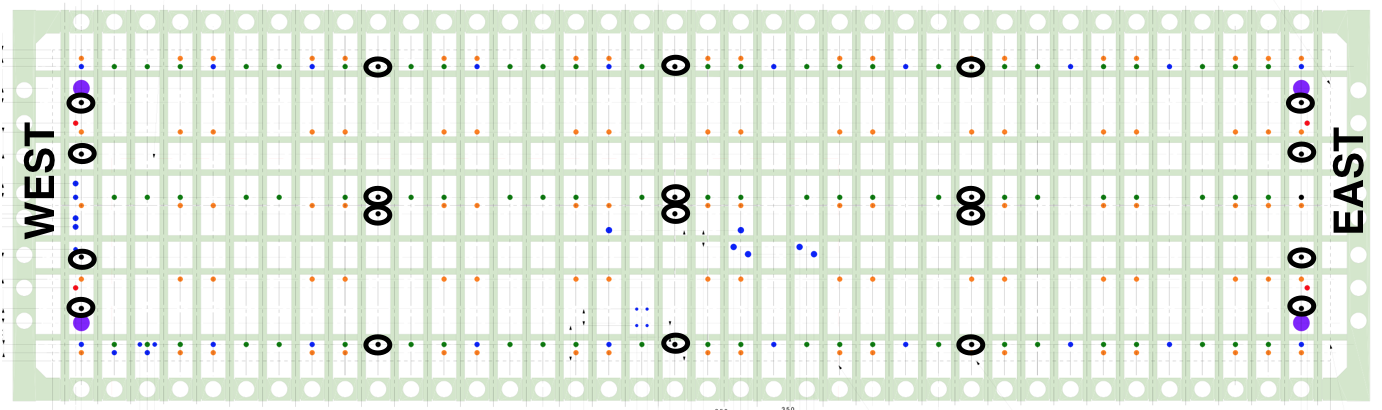
\includegraphics[height=2.0in]{FTmap.png}
%\caption{Top view of the \spmod %DUNE SP FD 
%cryostat showing various penetrations. Circles highlighted in black are multi-purpose calibration penetrations. The green dots are \dword{tpc} signal cable penetrations. The blue ports are cryogenic ports. The orange ports are \dword{dss} penetrations. The larger purple ports at the four corners of the cryostat are human access ports.}
%\label{fig:ftmap}
%\end{figure}

\begin{dunefigure}[Sketch of cryostat penetration map with laser calibration ports]{fig:DPFDLaserPositions}
{Top view of the \dpmod %DUNE SP FD 
cryostat showing possible laser system penetrations (black circles). The red line shows the \dword{fc} top view and the green square is one of the six \dword{crp} modules. 
%Circles highlighted in black are multi-purpose calibration penetrations. The green dots are \dword{tpc} signal cable penetrations. The blue ports are cryogenic ports. The orange ports are \dword{dss} penetrations. The larger purple ports at the four corners of the cryostat are human access ports.
}
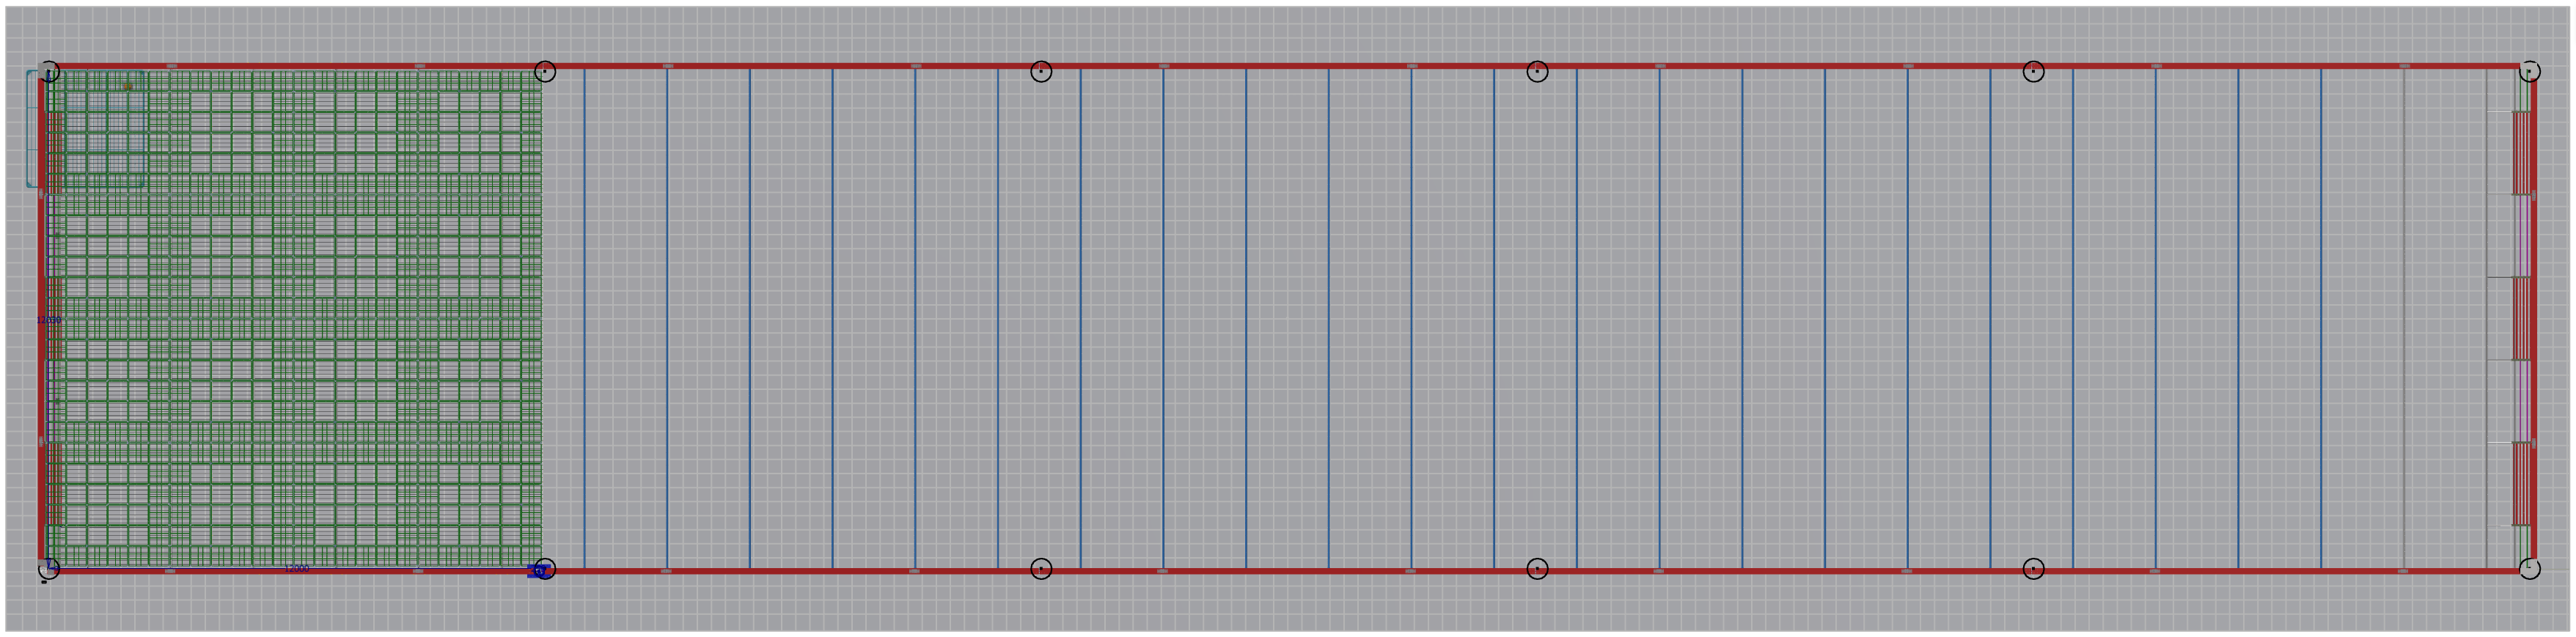
\includegraphics[width=1.0\textwidth]{DPFDLaserPositions.png}
\end{dunefigure}


The placement of these penetrations is driven by requirements of the ionization laser system and the available gaps between \dword{crp} and \dword{fc}.
%and radioactive source system. 
%The ports that are %inwards 
%towards the center of the cryostat are placed near the \dwords{apa} to minimize any risks due to the \dword{hv} discharge. For the far east and west ports, \dword{hv} is not an issue as they are located outside the \dword{fc} and the penetrations are located near mid-drift (location favorable to possible source deployment).
%to meet radioactive source requirements. 
%\fixme{The amendment above may need some work. I won't look at it until it's ready.}
Implementing the ionization laser system as proposed in Section~\ref{sec:dp-calib-sys-las-ion} requires \num{12} feedthroughs at each of the indicated ports. 
%the four \dword{tpc} drift volumes; this arrangement allows lasers to be used for full volume calibration of the E field and associated diagnostics (e.g., \dword{hv}). 

The distance between any two consecutive feedthrough columns in Figure~\ref{fig:DPFDLaserPositions} should be approximately \SI{12}{\m}, which is reasonable because experience from the \dword{microboone} laser system shows that tracks will propagate over that detector's full \SI{10}{\m} length. Assuming that the effects of Rayleigh scattering and self-focusing (Kerr effect) do not limit the laser track length, this laser arrangement could illuminate the full volume with crossing track data.  Please note that, at this time, the maximum usable track length is unknown, and the full \SI{60}{\m} \detmodule  length may be covered by the laser system after optimization.

%The exact location of the \dword{pns} ports is not yet finalized, but two ports, each at 1/4 of the module length (along beam direction) from each side should be close to optimal. 

For the \dword{pns} system, two ports, each at 1/4 of the module length (along the beam direction) from each side should be close to optimal to provide necessary coverage.

For the proposed \dword{rsds} system, ports must be close to the end-walls. An advantage of this system in \dword{dp} is that the source movement is along the drift direction, so several runs can be taken at different positions along the drift coordinate, which is important to check the detector response.

Between \num{4} and \num{10} additional ports should be available for the \dword{pns} system (toward middle of the cryostat) and the proposed \dword{rsds} system (close to the east and west end-walls). The exact locations of these additional ports is not yet finalized.

%\end{comment}


%%%%%%%%%%%%%%%%%%%%%%%%%%%%%%%%%%%%%%%%%%%%%%%%%%%%%%%
%\cleardoublepage

\section{Calibration Systems}
\label{sec:dp-calib-sys}

\dword{dune} plans to build two primary systems dedicated to calibrating the \dword{dp} far detector \dword{tpc}: a laser system
and a \dword{pns} system. The laser system should determine the \efield, mapping an essential parameter for describing the detector performance. 
Two laser systems are planned. 
With a high intensity laser, charge can be created in long straight tracks in the detector by direct ionization of \dword{lar} with the laser beams. This is described in Section~\ref{sec:dp-calib-sys-las-ion}. 
On the other hand, laser excitation of targets placed close to the cathode creates additional charge from well-defined locations that can be used to monitor the \dword{tpc}. This is described in Section~\ref{sec:dp-calib-sys-las-pe}. 
The \dword{pns} system is used to validate the low energy regime. This is described in detail in Section~\ref{sec:dp-calib-sys-pns}.

The physics motivation, requirements and design of these systems are described in the following subsections. 
%Alternative designs
%Non-baseline alternatives 
%for the ionization laser system, as well as 
The proposed radioactive source deployment system is described in the Appendix, in Section \ref{sec:dp-calib-sys-rsds}.

%\subsection{Ionization Laser System}
%\label{sec:dp-calib-sys-las}

%Two laser systems are planned. With a high intensity laser, charge can be created in long straight tracks in the detector by direct ionization of \dword{lar} with the laser beams. This is described in Section~\ref{sec:dp-calib-sys-las-ion}. On the other hand, laser excitation of targets placed in the cathode creates additional charge from well-defined locations that can be used to monitor the TPC. This is described in Section~\ref{sec:dp-calib-sys-las-pe}.
%The next sections describe the two subsystems based on these effects.

%%%%%%%%%%%%%%%%%%%%%%%%%%%%
\subsection{Ionization Laser System}
\label{sec:dp-calib-sys-las-ion}
%%%%%%%%%%%%%%%


Through its effect on drift velocity, recombination, and lifetime, the \efield is a critical parameter for physics signals as it ultimately affects the spatial resolution and energy response of the detector. The primary purpose of a laser system is to provide an independent, fine-grained estimate of the \efield in space and time. It would be extremely valuable to achieve measurements of electron lifetime with the laser system, but the feasibility of that is still under discussion.
The R\&D plan in \dword{pddp} will address the feasibility of carrying out charge-based measurements which, if successful, would open up the possibility of using the laser to measure electron lifetime. So, except where specifically indicated, the rest of this section will focus on drift velocity and \efield measurement.

\subsubsection{Physics Motivation}
Because it measures spatial distortions of straight tracks, the laser system actually measures the local drift velocity field directly and helps define the detector \dword{fv}, and this in itself is an important input for the \dword{lbl} analysis. 
%, and this is in itself an input to the analysis.
%Still,
However, it is still important to use information independent of the charge in order to disentangle effects like lifetime and recombination from \efield distortions. The laser system can do this, by using the position information to derive the \efield from the local velocity map, taking into account the colinearity between both vectors, and the relatively well studied relation on the magnitude (see~\cite{Li:2015rqa} and references [29, 45-58] therein). A laser system also has the intrinsic advantage of being immune to recombination, thus eliminating particle-dependent effects.  


Several sources may distort the drift \efield temporally and/or spatially in the detector. Positive ion accumulation and drift (space charge) due to ionization sources like cosmic rays or \Ar39 should be significant in the \dword{dune} \dword{dp} \dword{fd} module. Current simulation studies indicate that, considering only the accumulation of positive ions created in the liquid phase, we should expect \efield distortions of at most \SI{1}{\%}~\cite{bib:mooney2018}. Because of the longer drift length this is already significantly more than the \SI{0.1}{\%} expected in \dword{sp}. In addition, a fraction of the positive ions created in the gas phase amplification stage can drift back into the liquid and cause even more distortion. Current studies\footnote{These studies are based on the following assumptions: \dword{lem} gain of \num{100}; \SI{10}{\%} of the ions from gas phase drift into \lar; ion drift velocity of \SI{8}{\milli\metre\per\s}.} indicate that the \efield distortion caused by space charge, including ion feedback, can reach \SI{15}{\%} of the nominal field~\cite{bib:yu2018a}.
Furthermore, this effect may be enhanced or spatially distorted because of possible stable eddies in the \dword{lar} fluid flow. A \SI{15}{\%} distortion can lead to spatial distortions of \SI{1.2}{\metre} and temporal distortions of \SI{0.1}{\milli\s}, which are very significant compared to \dword{sp}. 
%KMTDRREADME: most 1% => at most 1%

%However, not enough is known yet about the fluid flow pattern in the \dword{fd} to exclude the possibility of stable eddies which may amplify the effect for both \single and \dual modules. This effect can get further amplified significantly in the \dword{dpmod} due to  accumulation in the liquid of ions created by the electron multiplication process in the gas phase.
%due to ion accumulation at the liquid-gas interface. 
Additionally, other sources in the detector (especially detector imperfections) can cause \efield distortions. For example, \dword{fc} resistor failures (see Figure~\ref{fig:efield_resistorfailure_mooney2019}), non-uniform resistivity in the voltage dividers, and misalignment or structural deformations of the cathode grid can create localized \efield distortions. These effects should be less pronounced than in the \dword{sp} because there are fewer detector elements within the \dword{tpc}, but also because in the \dword{dp} system, four resistors would have to fail to cause a failure across the \dword{fc} gap.

%\begin{dunefigure}[Impact on \efield of \dword{cpa} position distortions]{fig:efield_cpa_distortions_boyu2017}
%{Illustration of a possible distortion of the \dword{cpa} position~\cite{bib:yu2017a}, assuming a \SI{2}{\cm} swing, and its impact on \efield (right).}
%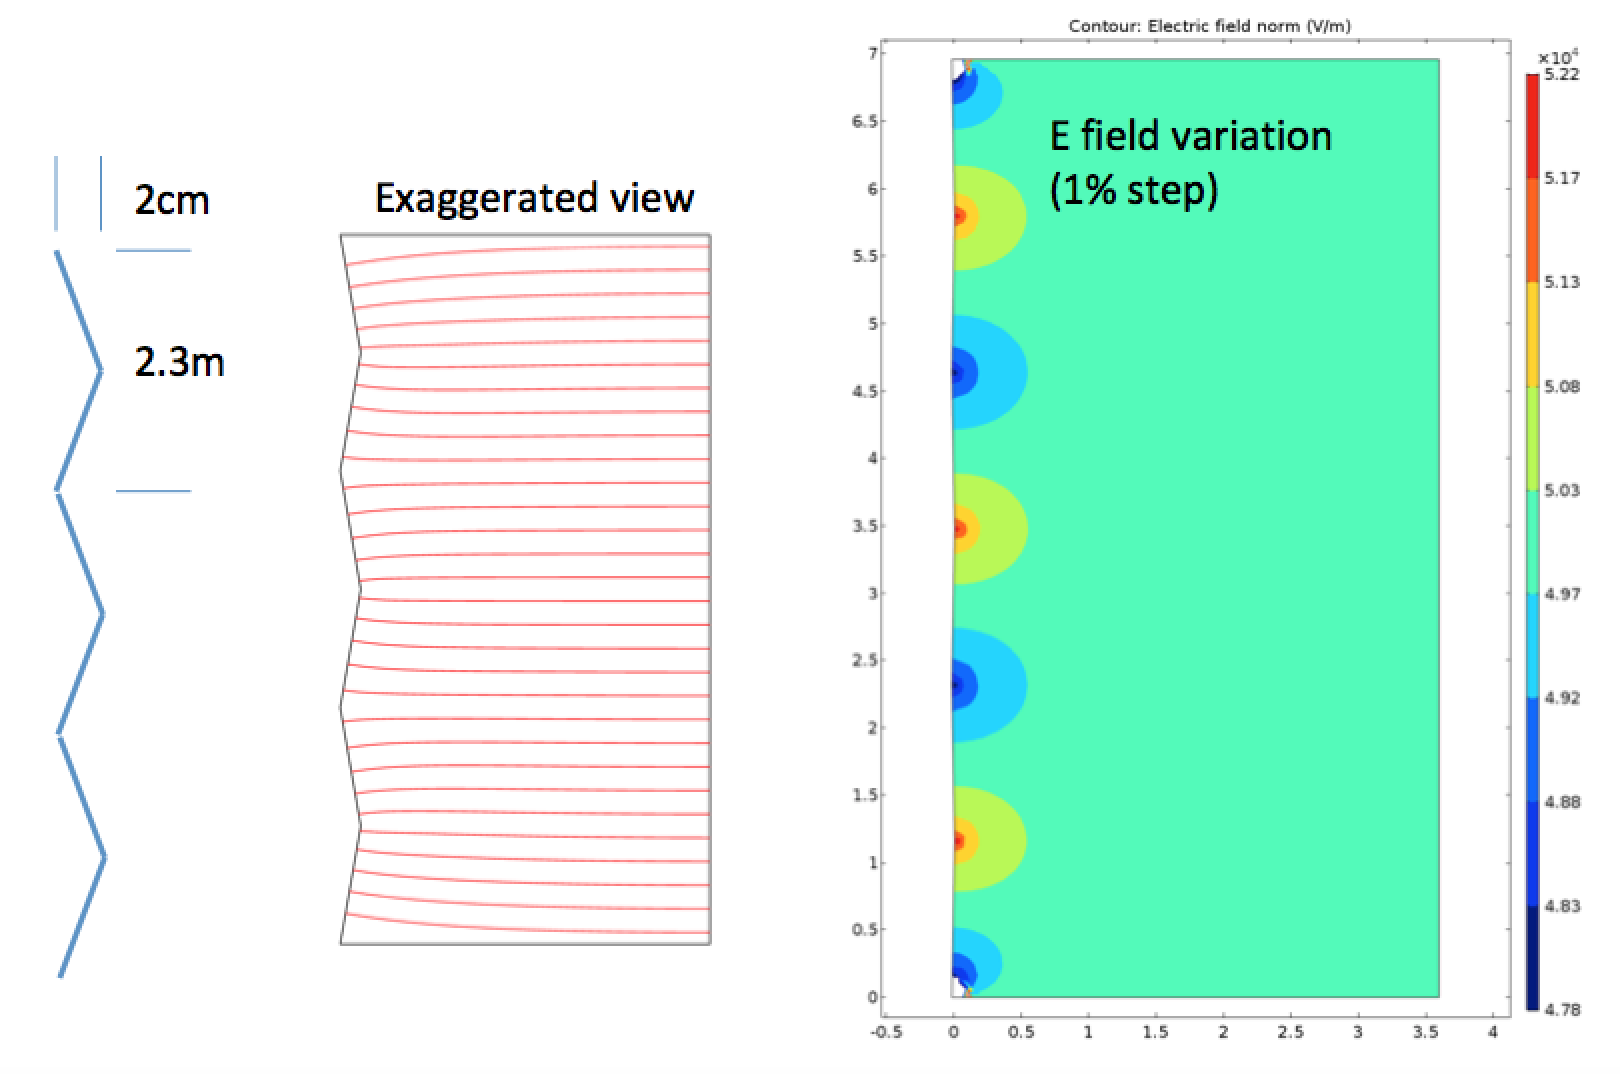
\includegraphics[width=0.8\textwidth]{efield_cpa_distortions_boyu2017.png}
%\end{dunefigure}

\begin{dunefigure}[Effect on \efield of  \dshort{fc} resistor failures]{fig:efield_resistorfailure_mooney2019}
{Effect on \efield magnitude distortions of a single \dword{fc} resistor failure in \dword{pdsp}~\cite{bib:mooney2019a}; shown as an example. 
%Caveat: Calculation done for \dword{sp}.
}
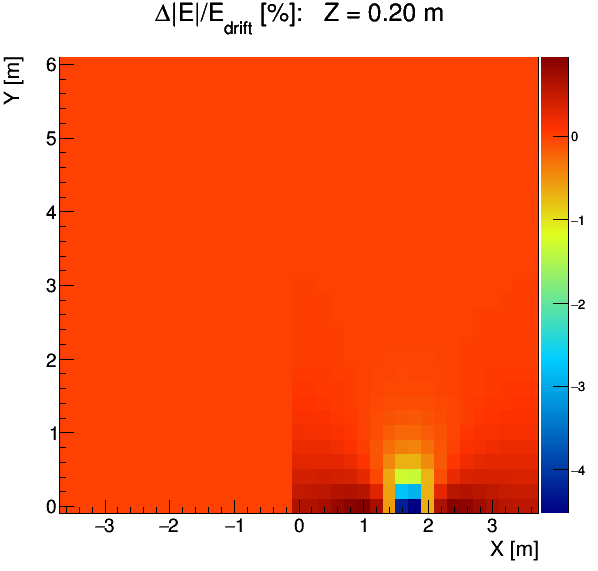
\includegraphics[width=0.5\textwidth]{efield_resistorfailure_mooney2019.png}
\end{dunefigure}

%In both \single and \dual systems, the failure of a resistor will create significant, local electric field distortions which will need to be identified\footnote{In the \dual system, four resistors would have to fail to cause a failure across the field cage gap, but even one failure in the SP can have an impact; this may be partially mitigated by modifying the HV, but not completely.}. While the resistor failure will be detected temporally, its location in space is not possible to determine from slow controls monitoring data. Misalignments of detector objects or deformations may also create (small) electric field distortions; while individual effects may be small, it is possible to have a combined, significant effect.

%KMTDRREADME, removed the 15% which seemed redundant with above.
Even if ion feedback space charge is expected to be the dominant \efield distortion effect,
%by up to \SI{15}{\%},
each individual \efield distortion may contribute, causing localized effects that must be understood with \textit{in situ} measurements of \efield for proper calibration. 

The laser system have many useful secondary uses as well, including alignment (especially for modes weakly constrained by cosmic rays),
%; see Figure~\ref{fig:apacurtainalign}),
stability monitoring, and diagnosing detector performance issues
%failures 
(e.g., \dword{hv}).  
%Misalignment may include physical deformation and/or rotations of objects within the detector.
Given the expected low rate of cosmic ray events (about 3500/day/10-kt) at the underground location, calibration with cosmic rays is not possible over short time scales. 
%KMTDRREADME: Add duration of timescale? Maybe "A 1% measurement is possible on a year timescale" Do we want to comment on rotation elements? Are there any?

%A laser system also has the intrinsic advantage of being immune to recombination, thus eliminating particle-dependent effects.  

With respect to electron lifetime, the preliminary results from \dword{pdsp} purity monitors and cosmic ray analyses indicate significant variations with time and space, both between monitors at different vertical coordinates (see \dword{tdr} \spchcisc), and between the regions inside and outside the \dword{tpc}. The possibility of carrying out such measurements with the ionization laser is therefore quite interesting. The ArgonTUBE experiment obtained lifetime measurements with laser~\cite{Ereditato:2013xaa} compatible with the cosmic ray ones, but it is not clear yet if this is possible at very large scales, since the modelling of the density of ionization charge created along the tracks presents challenges related to the previously mentioned self-focusing. Therefore the characterization of the ionization charge density from laser tracks will be an important goal of the development plan in \dword{pddp}.



%%%%%%%%%%%%%%%%%%%%%%%%%%%%
\subsubsection{Requirements}
\label{sec:dp-calib-laser-req}

%\fixme{uncomment when spec table available.\\ JM: but the spec table is included in a previous section, within overview.tex. I think the name requirements.tex is misleading. I'm changing to laser-ionization-requirements.tex; SG: agreed.}

% KM outline
%% Requirements we are held to from other systems -- EB table -- see Jose's early talk
%% Targets for SN and LBL physics -- or just remind in other subsections? \fixme{KM: right now the targets for SN and LBL physics exist in the design sections.}
%% System must operate for a long time
    % SG: physics driven calibration requirements, need a table to connect calibration requirements to high level physics requirements, not easy, but we need to try

%\fixme{guidance coming soon!}

%\fixme{KM: adjusted to be specific to laser; SG: I have made some edits as well. JM: OK, signing off.}

%The DUNE physics requirements and the high level specifications of other existing systems are the driving motivation for the specifications of the performance of the dedicated calibration systems, described below. From those, and the constraints due to detector dimensions, etc, derive also the engineering specifications of each calibration system, described in each system's respective section.

%\paragraph{\efield measurements}
The energy and position reconstruction requirements for physics measurements lead to requirements on the necessary precision of the laser %calibration 
\efield measurement, its spatial coverage and granularity. The next sections discuss the rationale behind each requirement, which we take as the \dword{dune} specification.
%, with ALARA (or AHARA for the coverage) as goal.

\paragraph{\efield precision}

In the \dword{lbl} and high-energy range, \physchlbl of this \dword{tdr}
%the \dword{dune} physics \dword{tdr} 
states that the calibration information must provide approximately \num{1} to \SI{2}{\%} understanding of normalization, energy scale and resolution, and position resolution within the detector.
Because a smaller \efield leads to higher electron-ion recombination and therefore a lower collected charge, distortions of the \efield can introduce
%are one of the possible causes of an 
energy scale bias. To connect this
%that requirement 
to a specification for the necessary precision of the \efield measurement, we note that, via recombination studies~\cite{bib:mooney2018}, we expect a \SI{1}{\%} distortion on \efield to lead to a \SI{0.3}{\%} bias on collected charge.
Because other effects will contribute to the lepton energy scale uncertainty budget, we consider a goal for the 
%calibration 
laser system to measure the \efield to a precision of $\sim$\SI{1}{\%} so that its effect on the collected charge is well below \SI{1}{\%}.
This is also motivated by the need for consistency with the high level \dword{dune} specification for field uniformity throughout the volume due to component alignment and \dword{hv} system, set at \fielduniformity. As was mentioned in Section~\ref{sec:dp-calib-requirements}, in \dword{dp} the long drift length and the gas phase ion feedback will lead to larger space charge \efield distortions than in \dword{sp}, up to approximately \SI{15}{\%}, making it even more important in \dword{dp} to monitor the \efield although the precision requirement should be the same (\SI{1}{\%}), as determined by the physics requirements, not by instrumentation constraints.

With two other high-level \dword{dune} specifications, the \dword{crp} strip spacing (\dpstrippitch) and the front end peaking time (\fepeaktime), the effect of this \efield precision requirement on engineering parameters of the calibration laser system is discussed further %ahead, 
in Section~\ref{sec:dp-calib-sys-las-ion-meas}.

\paragraph{\efield measurement coverage:}

In practice, measuring the \efield  throughout the whole volume of the \dword{tpc} will be difficult, so we must establish a goal for the coverage and granularity of the measurement. 
Until a detailed study of the propagation of the coverage and granularity into a resolution metric is available, a rough estimate of the necessary coverage can be made as follows.

Assuming \SI{15}{\%} as the maximum \efield distortion from possible compounding multiple  effects in the \dword{dune} \dword{fd},
we can then ask what would be the maximum acceptable size of the spatial region uncovered by the calibration system, if a distortion of that magnitude (systematically biased in the same direction) were present. To keep the overall (average) \efield distortion at the \SI{1}{\%} level, then that region should be no larger than \SI{7}{\%} of the total \dword{fv}. Therefore, we need a coverage of \SI{93}{\%} or more.

In addition, we need to consider that the method used to estimate \efield distortions is based on obtaining position displacement maps~\cite{bib:uBlaser2019}, and that the comparison between the reconstructed and true direction of a single track does not %univocally %unequivocally 
unambiguously determine a specific displacement map. Having tracks coming from different origins crossing in the same position is a direct way to eliminate that ambiguity, since the displacement vector is given simply by the vector connecting the intersections of the two reconstructed and the two true tracks. A joint iterative analysis of several close-by tracks is the default method for all other positions, but the system design should allow for the maximum possible number of positions %where there can be 
for crossing tracks from different beams.


\paragraph{\efield measurement granularity:}

The Volume~\volnumberphysics~(\voltitlephysics) of this \dword{tdr} states that a \dword{fv} uncertainty of \SI{1}{\%} is required. 
This translates to a position uncertainty of \SI{1.5}{\cm} in each coordinate (see \dword{tdr} \spchapa). 
In the $y$ and $z$ coordinates, position uncertainty is given mainly by the \dword{crp} strip pitch, and since this is \dpstrippitch, the requirement is met even when added in quadrature to the estimated maximum lateral diffusion of \SI{4.4}{\milli\m}. In the drift ($x$) direction, the position is calculated from timing, and considering the electronics peaking time of \fepeaktime, the uncertainty should be even smaller.
%\fixme{This is not entirely clear, and I can't see how to rephrase it.}
%\fixme{JM: Re-tweaked, I think it's clearer now. Please remove both if OK.}

The position uncertainty, however, also depends on the \efield, via the drift velocity. Because the position distortions accumulate over the drift path of the electron, it is not enough to specify an uncertainty on the field. We must accompany it by specifying the size of the spatial region of that distortion. For example, a \SI{10}{\%} distortion would not be relevant if it was confined to a \SI{2}{\cm} region and if the rest of the drift region was at nominal field.

Therefore, what matters is the product of [size of region] $\times$ [distortion]. Moreover, one can distinguish distortions into two types:
\begin{enumerate}
\item Those affecting the magnitude of the field. Then the effect on the drift velocity $v$ is also a change of magnitude. According to the function provided in \cite{Walkowiak:2000wf}, close to \SI{500}{\V\per\cm}, the variation of the velocity with the field is such that a \SI{4}{\%} variation in field $E$ leads to a \SI{1.5}{\%} variation in $v$.
\item Those affecting the direction of the field. Nominally, the field $E$ should be along $x$, so $E = E_L$ (the longitudinal component). If we consider that the distortions introduce a new transverse component $E_T$, in this case, this translates directly into the same effect in the drift velocity, which gains a $v_T$ component, $v_T=v_L  E_T/E_L $, i.e., a \SI{4}{\%} transverse distortion on the field leads to a \SI{4}{\%} transverse distortion on the drift velocity.
\end{enumerate}

Thus, a \SI{1.5}{\cm} shift comes about from a constant \SI{1.5}{\%} distortion in the velocity field over a region of \SI{1}{\m}. For the \efield, that could be from a \SI{1.5}{\%} distortion in $E_T$ over \SI{1}{\m} or a \SI{4}{\%} distortion in $E_L$ over the same distance.

%From ref.~\cite{Abi:2018dnh}, page~4-53, 
\efield distortions can be caused by space-charge effects due to accumulation of positive ions caused by \Ar39 decays (cosmic ray rate is low in \dword{fd}), or detector defects, such as \dword{crp} or \dword{fc} misalignment, \dword{fc} resistor failures (Figure~\ref{fig:efield_resistorfailure_mooney2019}), and resistivity non-uniformities, among other things.
%~\cite{Abi:2018dnh}. 
These effects added in quadrature can be as high as \SI{4}{\%}. 
%From ref. ~\cite{bib:mooney2018}, 
The space charge effects due to \Ar39~\cite{bib:mooney2018} can be \SI{0.1}{\%} for the \dword{sp} and \SI{1}{\%} for the \dword{dp}, so in practice, these levels of 
%that kind of distortion 
distortions must cover several meters to be relevant.
Other effects due to \dword{fc} imperfections can be higher than those due to space charge, but they are also much more localized. If we assume no foreseeable effects would distort the field more than \SI{15}{\%}, and considering the worst case scenario (transverse distortions), then the smallest region that would produce a \SI{1.5}{\cm} shift is \SI{1.5}{\cm}/\num{0.15}~=~\SI{10}{\cm}. This provides a target for the granularity of the measurement of the \efield distortions in $y$ to be smaller than about \SI{10}{\cm}, with of course a larger region if the distortions are smaller. Given the above considerations, then a voxel size of \num{10}$\times$\num{10}$\times$\SI{10}{\cubic\cm} appears to be enough to measure the \efield with the granularity needed for a good position reconstruction precision. 
%In fact, since the effects that can likely cause bigger \efield distortions are the problems or alignments in the \dword{cpa} (or \dword{apa}), or in the \dword{fc}, it could be conceivable to have different size voxels for different regions, saving the highest granularity of the probing for the walls/edges of the drift volume.



\begin{comment}
\begin{dunetable}
[Calibration Requirements]
{p{0.5\textwidth}p{0.15\textwidth}p{0.15\textwidth}}
{tab:calibreq}
{Calibration Specifications and Goals}   
Requirement & Specification & Goal \\ \toprowrule
\efield measurement precision & < 1\% & ALARA \\ \colhline
\efield measurement coverage & > 93\% & AHARA \\ \colhline
\efield measurement granularity & < 10x10x10 cm & ALARA \\ \colhline
\end{dunetable}
\end{comment}



\subsubsection{Design}
\label{sec:sp-calib-sys-las-ion-des}
%\paragraph{Baseline design}

The design of the laser calibration system for \dword{dune} is largely based on the design of the system built for \dword{microboone}~\cite{microboone}, which in turn was based on several previous developments~\cite{Rossi:2009im,Zeller:2013sva,Ereditato:2014lra,Ereditato:82014tya}. A similar system was also built for \dword{captain}~\cite{Berns:2013usa} and in the near future, will be built for \dword{sbnd}~\cite{Antonello:2015lea}. Operation of the \dword{microboone} system has already taken place. A preliminary report was given in~\cite{bib:chen2018}, and more details on the data analysis are available in~\cite{bib:uBlaser2019}.
%\todo{link the reference once uB publishes the laser paper in 2019}

\paragraph{Design overview}
Ionization of \dword{lar} by laser can occur via a multiphoton process in which a two-photon absorption~\cite{Badhrees:2010zz} leads the atom to the excited states band, and a third photon can cause ionization. This can only occur with high photon fluxes, and so the lasers must provide pulse energies of \SI{60}{\milli\joule} or more within a few ns. Unlike muons, the laser beams do not suffer multiple scattering and travel along straight lines determined by the steering mirror optics. 
The basic measurement consists of %recording the laser beams 
generating laser ionization tracks in the \dword{tpc} and comparing the reconstructed tracks with the direction known from the steering hardware. 
An apparent curvature of the measured track is attributed to drift velocity, and therefore \efield, distortions (either in direction or magnitude).


%Send this to last section
%The first step in the analysis~\cite{bib:uBlaser2019} is to obtain a field of position displacements by comparing the known and reconstructed tracks. If two crossing tracks are used, the displacement vector is simply given by the vector connecting the point where the reconstructed tracks cross and the point where the known tracks cross. However, because those displacements can vary both in direction and magnitude, that determination is ambiguous if only one track is used in a given spatial region. An iterative procedure was developed by the \dword{microboone} collaboration~\cite{bib:chen2018,bib:uBlaser2019} to 
%still 
%obtain a displacement map from a set of several non-crossing tracks from opposite directions. Following this, a set of drift velocity field lines (also known as \efield lines) can be obtained from the displacement map, assuming that all charge deposits along a field line will be collected in the same position. Using the relationship between \efield and drift velocity~\cite{Li:2015rqa,Walkowiak:2000wf}, the magnitude of the \efield can then be obtained 
%as well 

While the Rayleigh scattering length for \SI{266}{\nano\m}  light is approximately \SI{40}{\m}, additional optics effects may limit the maximum practical range of laser beams of that wavelength to a distance smaller than that. Those can include the Kerr effect  due to the dependency of the refractive index on the \efield. In the presence of an intense field, such as that caused by the laser beam itself, the change in refractive index can lead to lensing, or focusing, that distorts the coherence of the beam\footnote{The Kerr effect is so far believed to be the cause of non-homogeneity of the ionization along the laser beam observed in \dword{microboone}, which prevents the use of the charge information. Its effect on the position measurement and \efield uncertainty has been studied by \dword{microboone}.}. 

Despite this, laser beams with lengths of \SI{10}{\m} in \dword{lar} have been observed in \dword{microboone}, and beams with \SI{20}{\m} lengths (possibly more) can be reasonably expected to obtain with a similar system. This has determined the choice of locating the calibration ports in the cryostat roof at \SI{12}{\m} intervals. The \dword{dune} \dword{dp} cryostat roof port map is not defined yet, but the calibration proposal will have two sets of \num{6} ports located above the north and south walls, for a total of \num{12} ports, as shown in Figure~\ref{fig:DPFDLaserPositions}.

\paragraph{Mechanical and optical design for a single port sub-system}

For each of %those 
the used calibration ports, a laser sub-system can be schematically represented by Figure~\ref{fig:uB_laser_schematic} (left) and consists of the following elements:
\begin{itemize}
    \item A laser box (see Figure \ref{fig:uB_laser_schematic}, right) that provides
    \begin{itemize}
        \item A Nd:YAG laser with the fourth harmonic option providing \SI{266}{\nano\m}, in intense \SI{60}{\milli\joule} pulses with about \SI{5}{\nano\s} width, with a divergence of \SI{0.5}{\milli\radian}. The Surelite SL I-10 laser\footnote{Amplitude Surelite\texttrademark{} https://amplitude-laser.com/wp-content/uploads/2019/01/Surelite-I-II-III.pdf} is a possible choice since it has been successfully used in the past in other experiments.
        \item An attenuator and a collimator to control the intensity and size of the beam;
        \item A photodiode that gives a \dword{tpc}-independent trigger signal;
        \item A low-power red laser, aligned with the UV laser, to facilitate alignment operations;
        \item A Faraday cage to shield the surrounding electronics from the accompanying electromagnetic pulse. %EM \fixme{EM is defined as emergency management in the common glossary. Perhaps this should be spelled out? (Anne agrees and fixed.}
    \end{itemize}
    \item A feedthrough (see Figure \ref{fig:uB_laser_ft}, left) into the cryostat that provides
    \begin{itemize}
        \item The optical coupling that allows the UV light to pass through into the cryostat directly into the liquid phase, avoiding distortions due to the gas-liquid interface and the gas itself;
        \item A rotational coupling that allows the whole structure to rotate while maintaining the cryostat seal;
        \item A periscope structure (see Figure~\ref{fig:uB_laser_ft}; Right) mounted under the rotating coupling that supports a mirror within the \dword{lar};
        \item The additional theta rotation of the mirror accomplished by a precision mechanism coupled to an external linear actuator;
        \item Both the rotation and linear movements of the steering mechanism read out by precision encoders.
    \end{itemize}
    
\end{itemize}

\begin{dunefigure}[\dshort{microboone} laser calibration system schematics]{fig:uB_laser_schematic}
{Left: Schematics of the ionization laser system in one port~\cite{Antonello:2015lea}. Right: Schematics of the laser box~\cite{microboone}.}
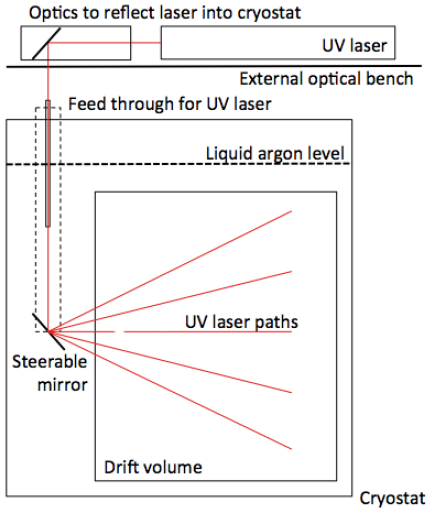
\includegraphics[width=0.45\linewidth]{uB_laser_schematic}
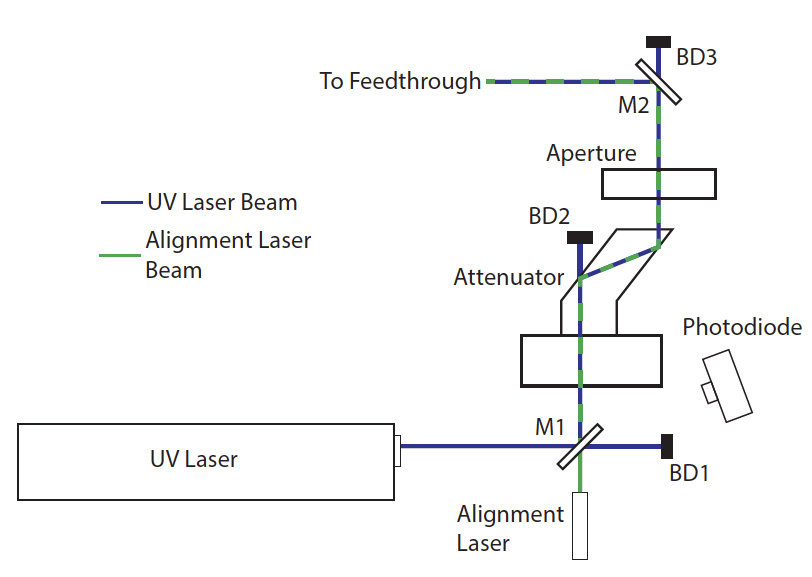
\includegraphics[width=0.5\linewidth]{uB_laser_box}
\end{dunefigure}

\begin{dunefigure}[\dword{microboone} laser calibration system drawings]{fig:uB_laser_ft}
{CAD drawings of the \dword{microboone} laser calibration system~\cite{microboone}. Left: calibration port feedthrough. Right: laser beam periscope. %Both figures from~\cite{microboone}.
}
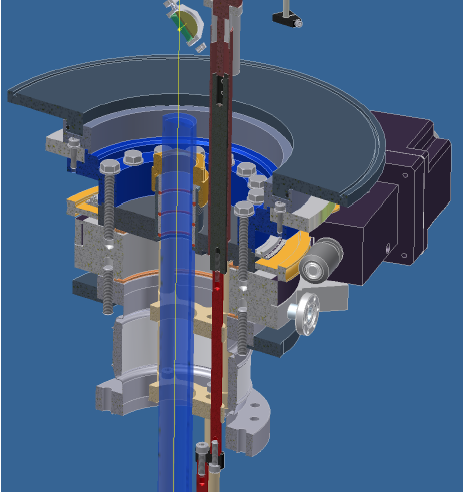
\includegraphics[width=0.49\linewidth]{uB_laser_ft}
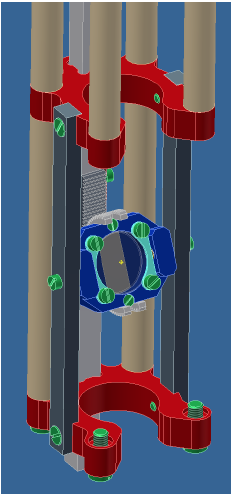
\includegraphics[width=0.248\linewidth]{uB_laser_periscope}
\end{dunefigure}

The baseline design will have the periscopes entering the top of the \dword{tpc} through the gap %space 
between the \dword{fc} and the \dword{crp} (see the views in figures \ref{fig:LaserPositionCorner} and \ref{fig:LaserPositionSide}). The brackets that connect the \dword{fc} structural elements (light grey and blue in the figures) must be adapted with suitable size holes that allow for the periscope size and a tolerance for the shifts due to \dword{fc} thermal shrinkage. This design allows \num{12} periscopes inside the \dword{tpc}, with no shadowing elements blocking the laser beams from covering the full volume.

\begin{dunefigure}[Laser calibration periscopes in the  \dword{dp} \dword{tpc} corner]{fig:LaserPositionCorner}
{CAD illustration of the calibration periscopes within the \dword{dune} \dword{dp} \dword{tpc} corner. Left: View from top. Right: View from bottom.}
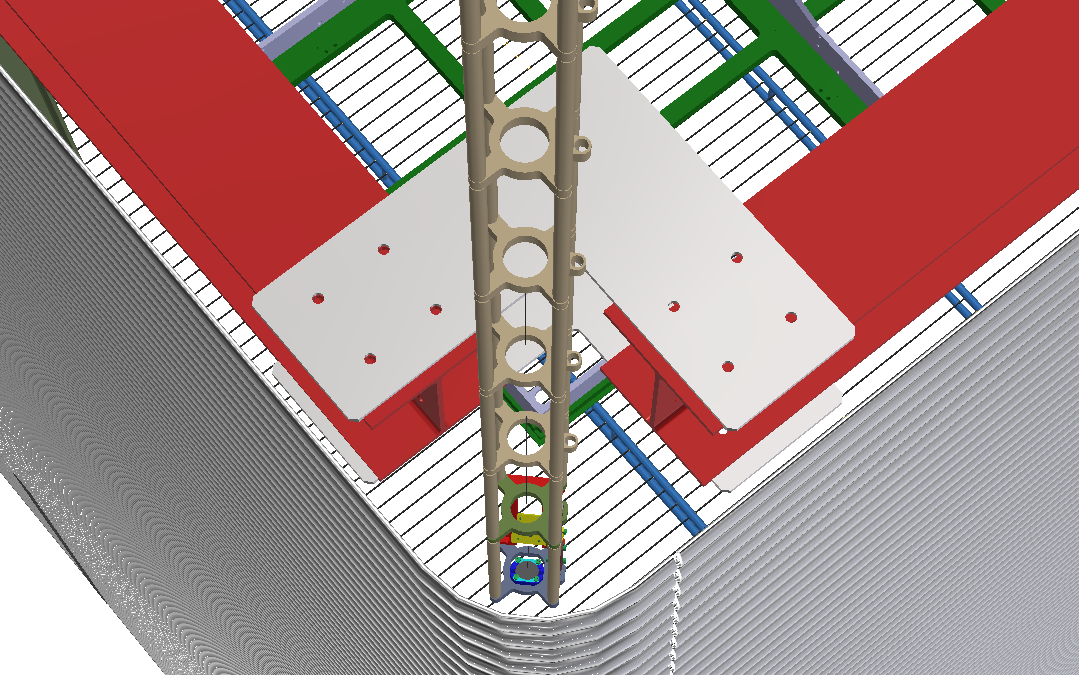
\includegraphics[width=0.49\linewidth]{LaserPositionCorner.png}
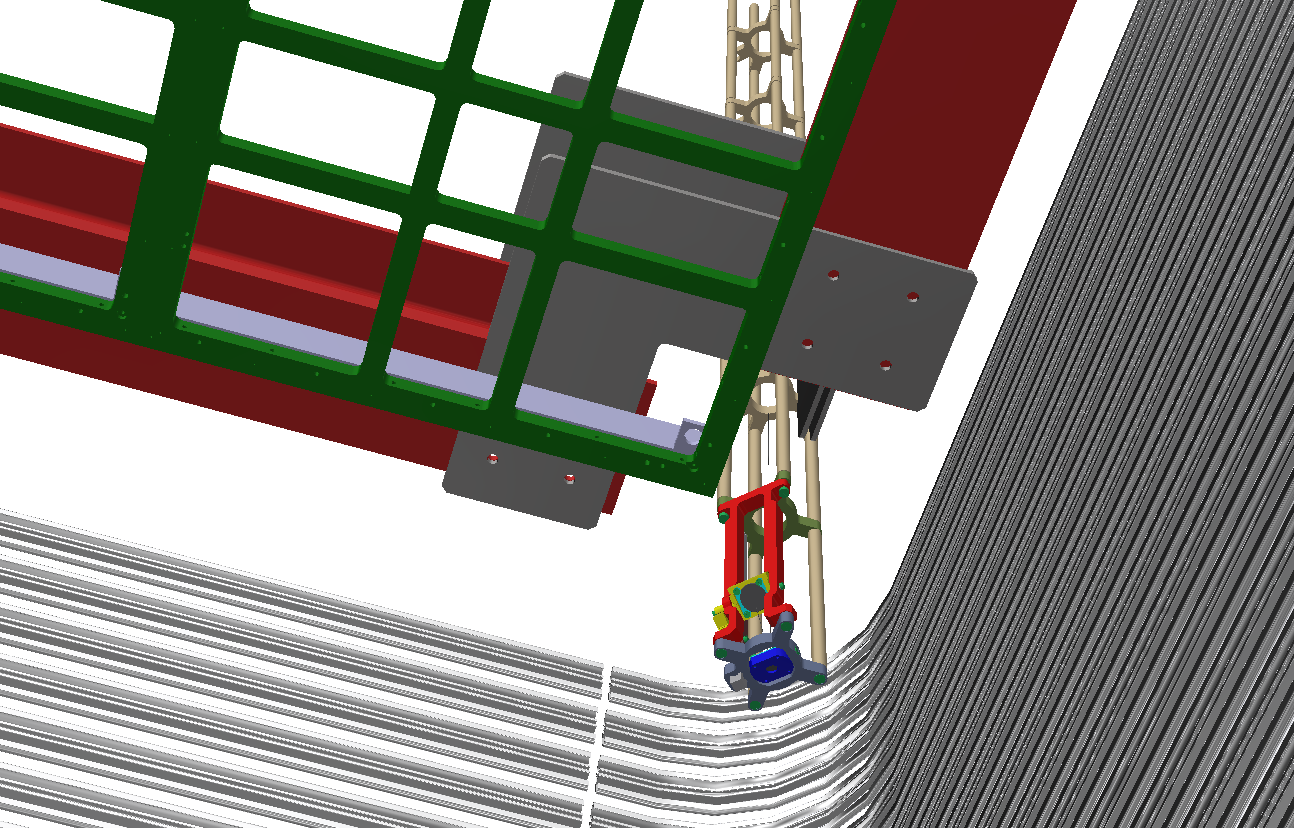
\includegraphics[width=0.49\linewidth]{LaserPositionCorner1.png}
\end{dunefigure}

\begin{dunefigure}[Laser calibration periscopes within the \dword{dp} \dword{tpc} side]{fig:LaserPositionSide}
{CAD illustration of the calibration periscopes within the \dword{dune} \dword{dp} \dword{tpc} side. 
%Left: Location on the corner. Right: Location on the side. 
Left: View from top. Right: View from bottom.}
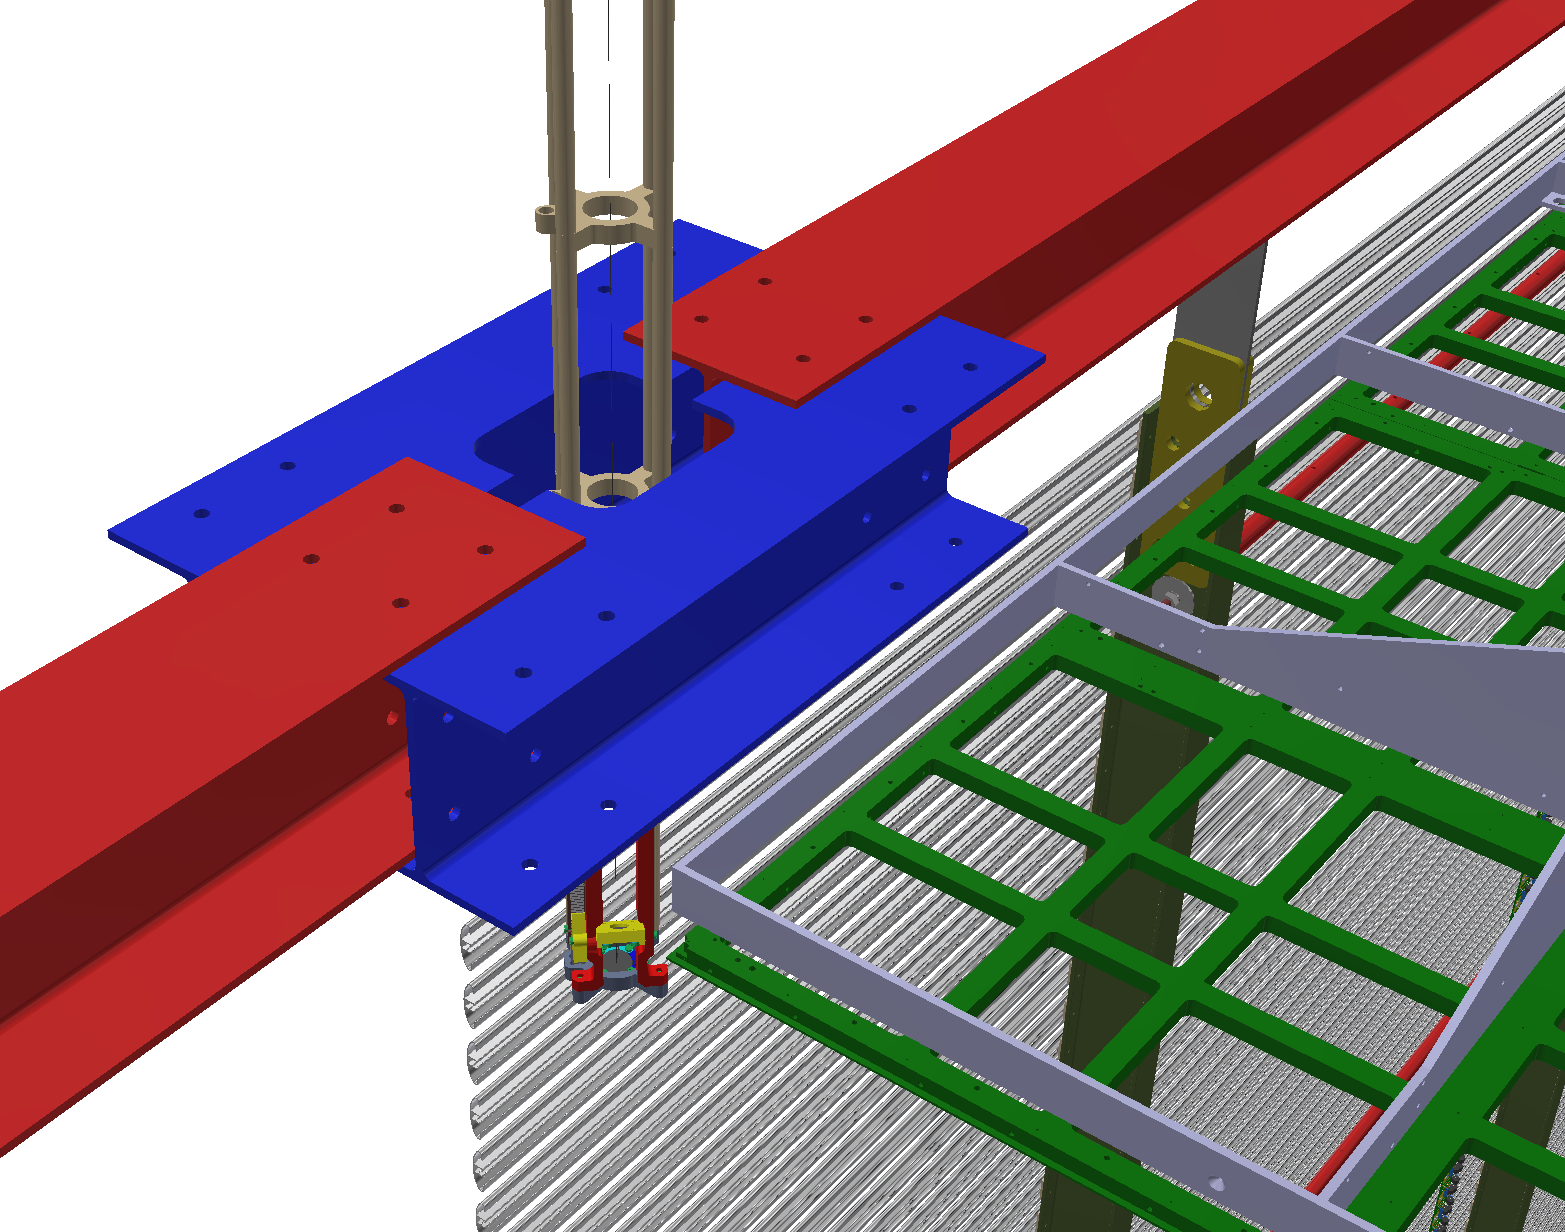
\includegraphics[width=0.49\linewidth]{LaserPositionSide.png}
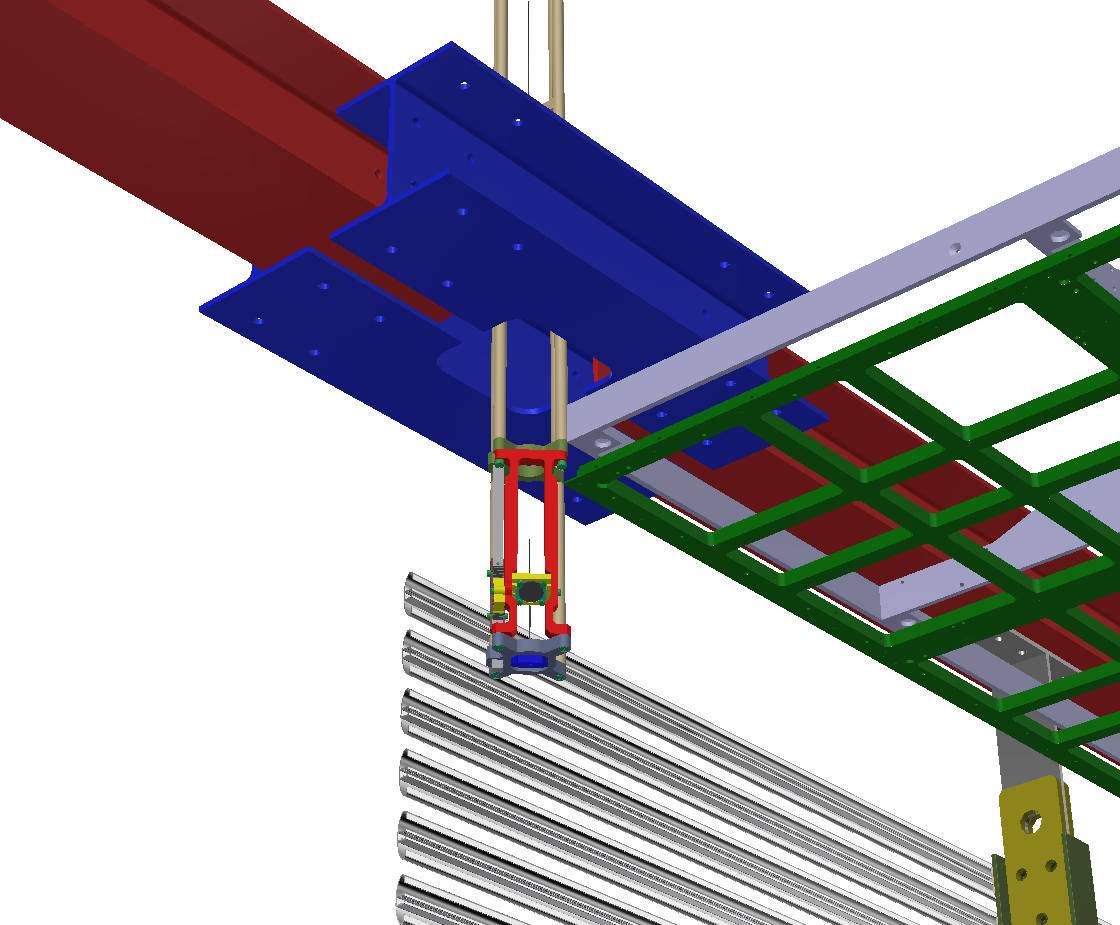
\includegraphics[width=0.49\linewidth]{LaserPositionSide1.png}
\end{dunefigure}


The goal of the mechanical design of the system is to achieve a precision close to that of the \dword{tpc} position measurements, so that no single factor dominates %in 
the overall systematics. The starting point of the laser beams is given by the position of the mirror in the periscope, which is known from construction drawings, warm surveys and cool down calculations. The angle of the beam is given by the angles ($\theta$, $\phi$) of the mirror, which are set by the periscope motors and read out by the encoders. 
For \dword{microboone}, reference~\cite{bib:chen2018} quotes a very good \SI{0.05}{\mrad} precision (\SI{0.5}{\milli\m} at \SI{10}{\m}) from the encoders alone, and an overall pointing precision of \SI{2}{\milli\m} at \SI{10}{\m}, driven mostly by beam size and divergence. In fact, with a \SI{0.5}{\mrad} divergence, we expect the beam to be \SI{5}{\milli\m} wide at \SI{10}{\m}.
In \dword{dune}, we aim to reach a similar precision. This will require a number of design and installation considerations: having encoders of similar high accuracy, carrying out surveys in various reference frames, and a capability to do location checks with a precision of about \SI{5}{\milli\m}  at \SI{20}{\m} from the beam origin. Therefore we aim to have a system that can locate the beam end point in few positions and attached to different references, at least one per drift volume and laser beam. The independent laser beam location system is described in Section~\ref{sec:dp-calib-sys-las-loc}. 

A scan of the full detector using \num{10}$\times$\num{10}$\times$\SI{10}{\cubic\cm} volume elements requires a number of tracks on the order of \num{4e5} and can take about two days. Shorter runs could be done to investigate specific regions. Sampling granularity, and therefore the amount of data taken, depends on \dword{daq} requirements. In fact, to even be able to record the desired \num{4e5} tracks, a dedicated data reduction algorithm must be devised, so that only a drift window of approximately \SI{100}{\micro\s}
of data is recorded; the position of that window depends on beam position as well as the direction and \dword{crp} sections being read out. More details on this are given in Section~\ref{sec:dp-calib-daqreq}.



%%%%%%%%%%%%%%%
\subsubsection{Measurement Program}
\label{sec:dp-calib-sys-las-ion-meas}

This section describes the methods used to measure 
%drift velocity and \efield 
parameter maps and their expected precision, given the design outlined above.

\paragraph{\efield and drift velocity measurement}
The method for \efield measurement is based on the measurement of apparent position displacements of the straight laser tracks. The laser produces straight tracks with a known starting position and direction. If, when reconstructed under the assumption of uniform and homogeneous drift velocity, any deviations from that are observed, they are attributed to \efield distortions. 

The first step in the analysis~\cite{bib:uBlaser2019} is to obtain a field of position displacements by comparing the known and reconstructed tracks. If two crossing tracks are used, the displacement vector is simply given by the vector connecting the point where the reconstructed tracks cross and the point where the known tracks cross. However, since those displacements can vary both in direction and magnitude, there will be ambiguity in that determination if only one track is used in a given spatial region. An iterative procedure was developed by the \dword{microboone} collaboration~\cite{bib:chen2018,bib:uBlaser2019} to obtain a displacement map from a set of several non-crossing tracks from opposite directions. Following this, a set of drift velocity field lines, which are the same as \efield lines, can be obtained from the displacement map, assuming that all charge deposits along a field line will be collected in the same position. Using the relationship between \efield and drift velocity~\cite{Li:2015rqa,Walkowiak:2000wf}, we can then also obtain the magnitude of the \efield.

Since the observed position distortion in one location depends on \efield distortions in many locations along the drift path, this method of analysis clearly requires the acquisition of data from many different tracks crossing each detector drift volume at many different angles. 

Therefore, the precision with which the \efield distortions can be measured depends on the precision with which we can know the laser track position and the \dword{tpc} position reconstruction precision.
The \dword{tpc} precision in the $y$, $z$ coordinates is given primarily by the \dword{crp} strip spacing of \dpstrippitch and lateral diffusion, which can be up to \SI{4.4}{\milli\m} for the maximum drift of \dpmaxdrift and nominal \efield of \dpnominaldriftfield.
It is slightly better than that (approximately \SI{2}{\milli\m}) on the $x$ (drift) coordinate, determined by the \fepeaktime peaking time of the front-end electronics.
Given infinite laser positioning accuracy, the smallest measurable \efield distortions would be those that cause displacements of approximately \SI{2}{\milli\m} in $x$ and \SI{5}{\milli\m} in $y$, $z$. The precision for the drift velocity distortions depends on the size of the spatial region where they are present. For distortions present in regions of \SI{0.5}{\m} and larger, drift velocity distortions can therefore be measured with an accuracy of \SI{1}{\%} in $y$, $z$ and \num{0.4}\% in $x$. In $y$, $z$, \SI{1}{\%} precision on drift velocity distortions translates to \SI{1}{\%} precision on the transverse field distortions. Along $x$, one must consider that, at \dpnominaldriftfield, a \SI{1}{\%} change in \efield leads to a \SI{0.375}{\%} change in drift velocity. Therefore, finally, this means that the smallest measurable distortions given the \dword{tpc} design (\dword{crp} pitch, timing precision) are \SI{1}{\%} in \efield if they are present in regions of \SI{0.5}{\m} and larger. Smaller field distortions could in principle be measurable if they are present over larger regions because their effect accumulates over the drift path.
On one hand, this gives us an ultimate limit to the \efield precision achievable with the laser system, but on the other hand, because these \dword{tpc} precision considerations apply to physics events also, this tells us an \efield precision much more than \SI{1}{\%} should not have an effect on physics.

\paragraph{Charge-based measurements}

Electron drift-lifetime~\cite{bib:uBlifetime, Antonello:2014eha} is the parameter that governs the dependence of the amount of collected charge on the drift time. A possible measurement of electron drift-lifetime would therefore require a very good control over the charge profile of the ionization laser tracks. This was achieved in a small scale experiment that measured lifetime with laser beams~\cite{Ereditato:2013xaa}, but is harder with longer distances. The charge produced by the laser tracks along its path depends on distance because the light intensity is reduced due to beam divergence and scattering, as well as non-linear effects such as the self-focusing, or Kerr effect. For this reason, the first steps in any laser-based charge measurement are a fine-tuning of the laser intensity in order to reduce self-focusing to a minimum, and ``charge profile calibration scan'' which consists of acquiring tracks parallel to the \dword{crp}. In order to get good statistical precision, several tracks could be acquired, in the same or different direction, but always parallel to the \dword{crp} in order to factorize out any effect from electron drift-lifetime. This set of data provides a calibrated laser beam charge profile that can then be used to analyse and normalize the measured charge profile from tracks that do have an angle with respect to the \dword{crp} and therefore span different drift times.

As for electron-ion recombination, since the $dE/dx$ for laser beams is much smaller than for charged particles, the effect should also be much smaller. However, that small effect has been observed~\cite{Badhrees:2010zz}, so a similar method than described above could be used to evaluate any dependence of the electron-ion recombination factor on the angle $\phi$ between the track and the electric field, that is predicted in some models~\cite{Acciarri:2013met}. This would entail taking data with tracks as parallel as possible to the \efield, in order to enhance the angular dependence term on the recombination expression (that goes with $1/sin \phi$), and to compensate for the smaller $dE/dx$ for laser beams.








%%%%%%%%%%%%%%%%%%%%%%%%%%%%
\subsection{Laser positioning system}
\label{sec:dp-calib-sys-las-pos}


Because the precision of the \efield measurement relies heavily on a precise knowledge of the laser beam tracks, independent measurements of their directions for some specific positions is required. The laser positioning system addresses this. %KMTDRREADME: Need to remove the word requriement here?
%\subsubsection{Physics Motivation}
While the direction of the laser beam will be very well known from the reading from the encoders on the laser beam steering mechanism,  residual uncertainty, or unpredictable shift, in the pointing direction will remain. 
%Having 
%KMTDRREADME: %Keeping in mind  -> Given
Given the long length of the ionization track, more than \SI{12}{\m}, even a small offset in the pointing direction can lead to vastly different ionization track locations, especially close to the end of the track. Such inaccuracies will directly affect the ability to precisely calibrate any variations in the \efield.

\subsubsection{Design}

The laser positioning system (LPS) \fixme{This abbreviation is not in the glossary? Is it necessary?} is designed to address the problem of precise and accurate knowledge of the laser track coordinates. %University of Hawaii group has 
Two complementary systems are planned, one based on pin diodes and the other on mirrors.

\paragraph{Pin-diode system for laser positioning:}

A system based on pin diodes 
%(consisting of 1$\times$3) array 
was built for the mini\dword{captain} experiment; the installed version is visible in the photo of the mini\dword{captain} \dword{tpc} in  Figure~\ref{fig:LPS_miniCAPTAINlabeled}.  

%\begin{figure}[htb!] 
%\centering 
%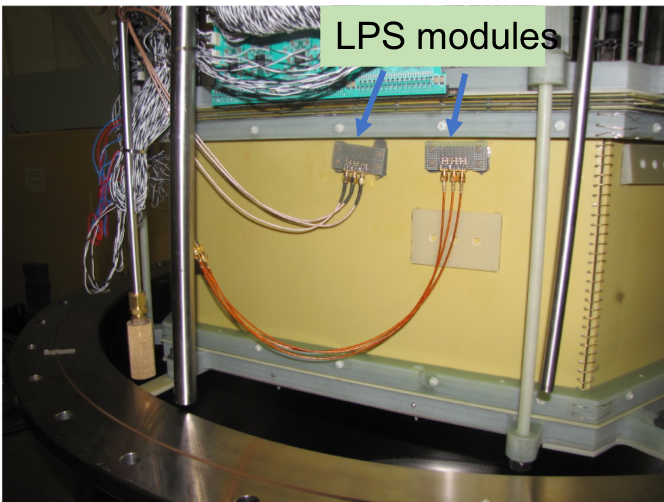
\includegraphics[width=0.6\linewidth]{LPS_miniCAPTAINlabeled.png} 
%\caption{Photo of the miniCAPTAIN TPC with two LPS modules glued on the outside to detect laser beam spot location via fluorescence of the TPC FR4 wall when illuminated by the laser beam.}
%\label{fig:miniCAPTAIN} 
%\end{figure}

\begin{dunefigure}[Laser positioning system modules in the miniCAPTAIN TPC]{fig:LPS_miniCAPTAINlabeled}
{Photograph of the mini\dword{captain} \dword{tpc} with two LPS modules glued on the outside to detect laser beam spot location via fluorescence of the \dword{tpc} FR4 wall when illuminated by the laser beam.}
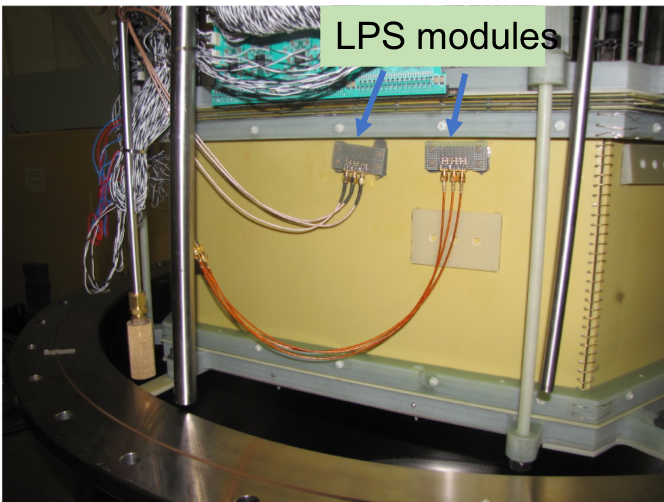
\includegraphics[width=0.6\linewidth]{LPS_miniCAPTAINlabeled} 
\end{dunefigure}

The LPS consists of groups of \num{9} pin diodes, operating in passive, photovoltaic mode. These are GaP diodes whose sensitivity range extends down to  \SI{200}{\nano\m} wavelength, so detecting \SI{266}{\nano\m} light is straightforward. Figure~\ref{fig:GaP_diode_room_temp} shows signals detected at room and cryogenic temperatures. The PIN diode was illuminated by the \SI{266}{\nano\m} light from the Nd:Yag
laser in the laboratory 
%(in the lab at University of Hawaii) 
set at lowest possible setting for minimal power. 

Pin diodes are placed at the bottom of the cryostat and receive light passing through the cathode and ground grids.
%gaps between the field cage profiles to minimize interference with the field cage. 
Drawings of one such group of pin diodes are shown in Figure~\ref{fig:GaP_assembly}. With the group of \num{9} photodiodes, not only can the beam be detected the beam but also its profile crudely characterized, giving a more precise location of the central beam pulse axis.


%\begin{figure}[htb!] 
%\begin{minipage}[b]{0.47\textwidth}
%\centering 
%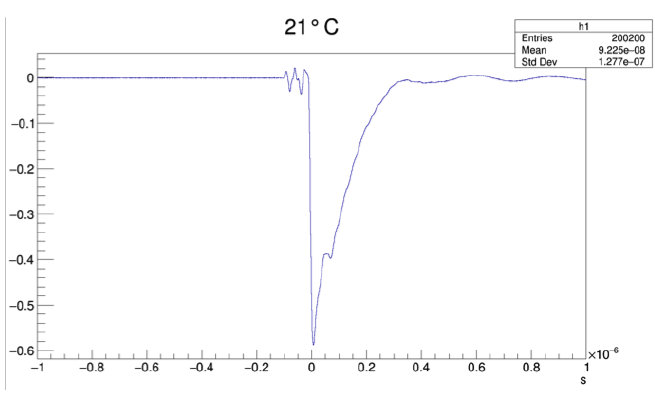
\includegraphics[width=0.95\linewidth]{GaP_diode_room_temp.png} 
%\caption{Signal from the GaP pin diode. The signal was a result of illumination of the PIN diode face with a 266\,nm laser at room temperature.}
%\label{fig:LPS1} 
%\end{figure}
%\end{minipage}
%\hfill
%\begin{minipage}[b]{0.47\textwidth}
%\begin{figure}[htb!] 
%\centering 
%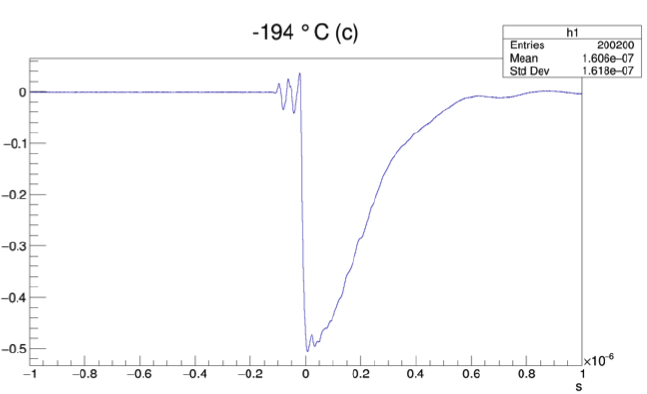
\includegraphics[width=0.95\linewidth]{GaP_diode_cryo_temp.png} 
%\caption{Signal from the GaP pin diode. The signal was result of illumination of the PIN diode face with a 266\,nm laser at cryogenic temperature.}
%\label{fig:LPS2} 
%\end{minipage}
%\hfill
%\end{figure} 


%\begin{figure}[htb!] 
%\begin{minipage}[b]{0.47\textwidth}
%\centering 
%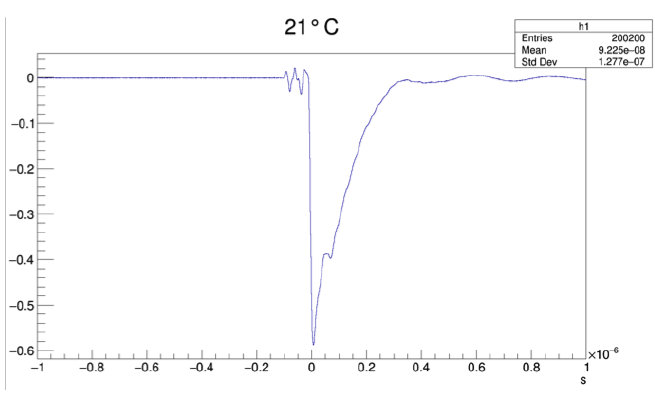
\includegraphics[width=1.0\linewidth]{GaP_diode_room_temp.png} 
%\caption{Signal from the GaP pin diode. The signal was a result of illumination of the PIN diode face with a 266\,nm laser at room temperature.}
%\label{fig:LPS1} 
%\end{minipage}
%\hfill
%\begin{minipage}[b]{0.47\textwidth}
%\centering 
%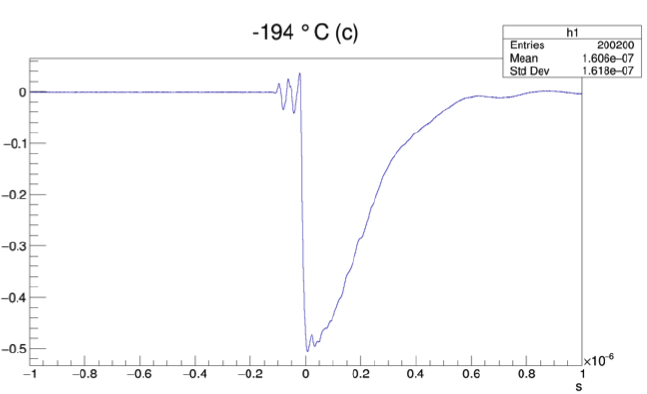
\includegraphics[width=1.0\linewidth]{GaP_diode_cryo_temp.png} 
%\caption{Signal from the GaP pin diode. The signal was result of illumination of the PIN diode face with a 266\,nm laser at cryogenic temperature.}
%\label{fig:LPS2} 
%\end{minipage}
%\hfill
%\end{figure} 


\begin{dunefigure}[Signal from the miniCAPTAIN laser positioning system at room and cryogenic temperatures]{fig:GaP_diode_room_temp}
{Signal from the miniCAPTAIN laser positioning system GaP pin diode. The signal was a result of illuminating the PIN diode face with a \SI{266}{\nano\m} laser at room (left) and cryogenic (right) temperatures.}
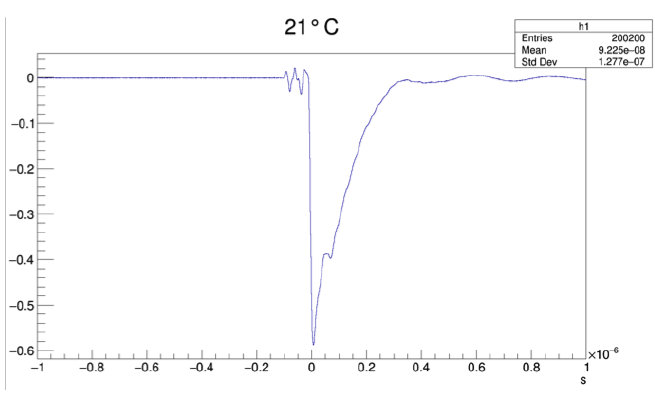
\includegraphics[width=0.47\linewidth]{GaP_diode_room_temp.png} 
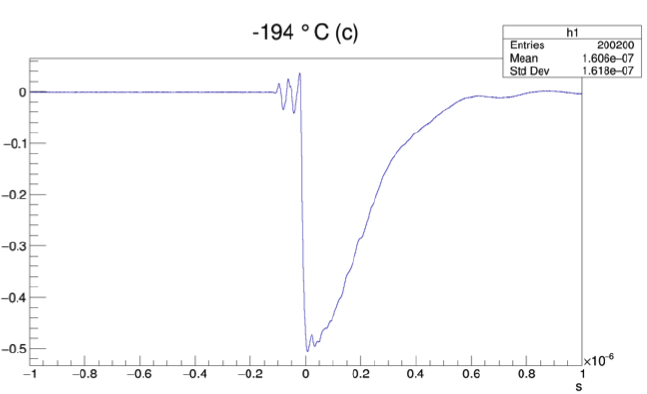
\includegraphics[width=0.47\linewidth]{GaP_diode_cryo_temp.png} 
\end{dunefigure}



\begin{dunefigure}[Cluster assembly of the miniCAPTAIN laser positioning system]{fig:GaP_assembly}
{(Left) LPS cluster mounted on the opposite wall from the laser periscope to detect and accurately determine the end point of the laser beam. (Right)
Profile of the LPS group mounted on the PCB. GaP diodes come with pins that use pairs of twisted wires to transport the signal.
}
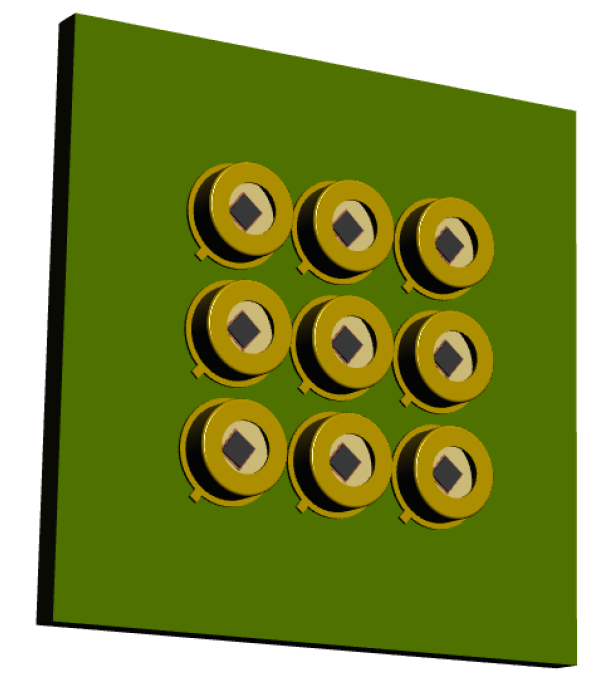
\includegraphics[width=0.47\linewidth]{GaP_assembly.png} 
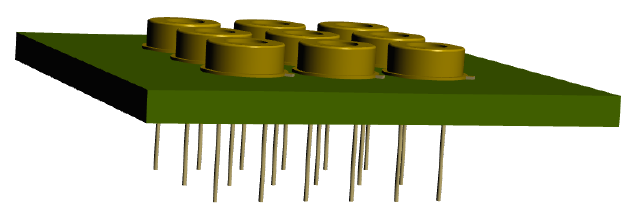
\includegraphics[width=0.47\linewidth]{GaP_assembly_profile.png} 
\end{dunefigure}


There will be one LPS pad per laser periscope. Laser always send the first pulse in the direction of the LPS before going into a calibration sequence. 
%The electronics used to collect signals from the LPS will be provided by \dword{cisc}.\todo{CISC doesn't provide electronics. SG emails Jelena to clarify this.}


\paragraph{Mirror-based beam positioning system:}

In addition to the pin-diode system, we will also have clusters of small mirrors that allow measuring the beam end position using its reflection.

Figure~\ref{fig:laser_mirror_positioning} shows a conceptual sketch with a cluster of 6 mirrors located close to each other but at different angles. When the beam hits one mirror, it will be reflected back into the \dword{tpc}, and the reflection angle unambiguously identifies which mirror was hit. Because the clusters of mirrors are small (a few cm), they fit inside the \dword{fc} profiles. With small mirrors, \SI{5}{\milli\m} in diameter, the required positioning precision would be met if these mirrors are placed at distances further than \SI{10}{\m}. The preferred location is, therefore, on the opposite \dword{fc} side wall. Because the top half of the \dword{fc} will be covered with \dword{pds} reflector panels, only lower half of the \dword{fc} profiles can be used. For redundancy, each laser periscope should have two associated mirror clusters, so the total number of clusters would be \num{32}. 

The simplest solution would be to have the reflecting surface made of polished aluminum, so the cluster could be a single block. Tests must be made of the actual reflectivity of the (oxidized) surface. An alternative would be small dielectric mirrors.

\begin{dunefigure}[Mirror-based laser beam positioning system]{fig:laser_mirror_positioning}
{View of the mirror cluster for the beam positioning system inserted in the \dword{fc} profiles~\cite{bib:yu2019a}.}
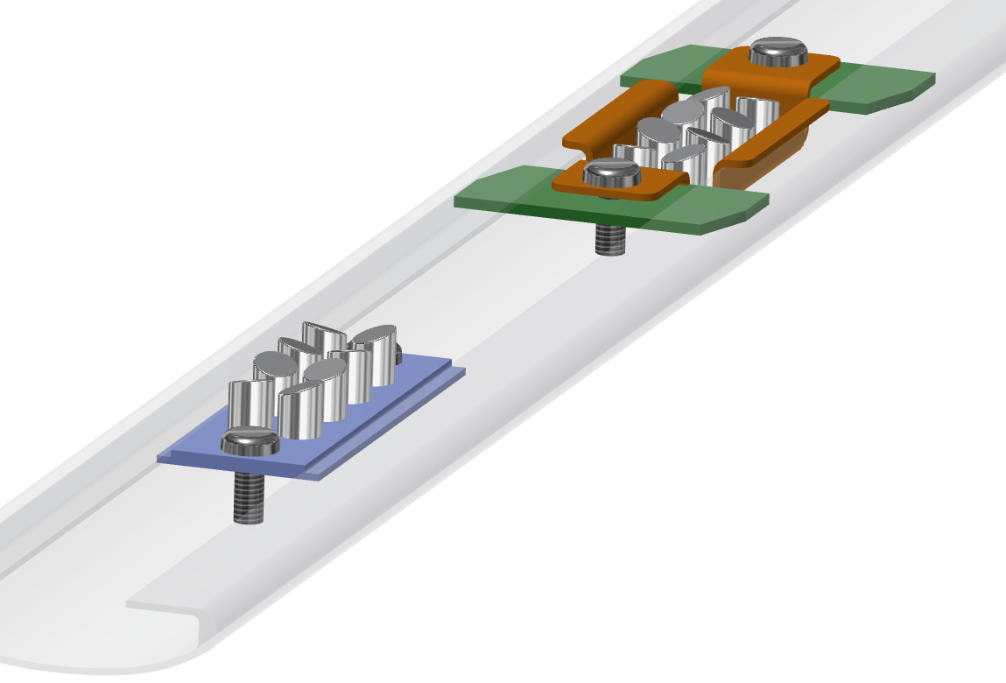
\includegraphics[width=0.7\linewidth]{laser_mirror_positioning.pdf}
\end{dunefigure}

\subsubsection{Development plan}
 The LPS assembly for reducing electronic noise and cross-talk must be further optimized, as must the size and shape of the cluster so that it would best collect the light coming through the cathode and ground grids.  Further, the system must be durable for extensive running under cryogenic conditions with  a large number of cool-downs to validate GaP for extended use in \dword{dune}. Finally, SiPMs are under consideration among other alternatives to GaP. While SiPMs require power, their sensitivity to single photons makes them desirable for low light signals and more accurate beam direction reconstruction. 
%KMTDRREADME:  What are noise rquirements and cross talk? 
%KMTDRREADME:  Does the LPS fail? Is it a big deal if it fails?
    

















%%%%%%%%%%%%%%%%%%%%%%%%%%%%
\subsection{Photoelectron Laser System}
\label{sec:dp-calib-sys-las-pe}
%\subsection{Photoelectron Laser System}
%\label{sec:dp-calib-sys-las-pe}
%\subsubsection{Physics Motivation}
%\label{sec:sp-calib-sys-las-pe-phys} 
Well localized electron sources are excellent calibration tools for studying electron transport in the \dword{lartpc}, identifying inhomogeneities in the \efield in all directions, and precisely determining the electron drift velocity. Verification and calibration of the \efield distortions are important for particle vertex reconstruction and identification and affect the associated systematic errors, leading to increased rate of mis-identification and poorer energy reconstruction. Photoelectron lasers can provide well localized electron sources on the cathode at predetermined locations for improved characterization of the \efield and consequent reduction of detector instrumentation systematic errors. Also, a photoelectron laser system, a simpler system operationally than ionization laser systems, can be used to quickly diagnose whether large sections of the detector are operational.
%KMTDRREADME, replaced above%can be used as a wake-up system to quickly diagnose if the detector is alive. 
This is especially important because of the low cosmic ray rates in the underground detector. 

\subsubsection{Design}
\label{sec:dp-calib-sys-las-pe-des}

To produce localized clouds of electrons using a photoelectric effect, small aluminum discs or thin discs with evaporated gold film, will be used as targets. As stated in reference~\cite{Li:2016ods}, gold film can be just \SI{22}{\nano\m} thick. Several photoelectric strips will complement the circular targets to calibrate the amount of transverse diffusion in \dword{lar}. Based on the experience from T2K and \dword{bnl} \dword{lar} test-stands~\cite{Li:2016ods}, \SIrange{8}{10}{\milli\m} diameter targets are sufficient. Targets placed close to the cathode and the distance between the dots will be determined based on the calibration needs and simulation outcomes. Nominally, dot spacing should be \SI{1}{\m} with photocathode strips every \SI{5}{\m}. The layout of the photoelectric dots and strips will be further refined using the calibration requirements and performance simulation results.  Conducting a survey of the photocathode disc locations on the cathode  after installation and before detector closing will be essential. In this way, the absolute spatial calibration of the electric field can be achieved.

At \SI{266}{\nano\m} Nd:Yag quadrupled wavelength, the single photon energy of \SI{4.66}{\eV} is sufficient to generate photoelectrons from aluminum, but not from gold, which requires two-photon absorption and therefore higher intensities.
%At S\I{266}{\nano\m} Nd:Yag quadrupled wavelength, the photon energy of\SI{4.66}{\eV} is sufficient to generate photoelectrons from both aluminum and gold. 
While aluminum has a lower associated cost, a gold film surface is easier to protect from contamination. 
%A couple of hundred electrons 
%A couple of thousand electrons 
A few thousand electrons are expected per spill from each dot. The laser beam will be 
%coming from the anode injection points, used as sources, 
guided to injection points via cryogenic optical fibers with defocusing elements on the other end. The fiber injection points will be mounted on the \dword{fc} or \dword{crp} to achieve the most efficient illumination of the targets on the cathode with minimal numbers of injection points. 

%\fixme{Jose M to Jelena M: Where can these injection points be? close to the CRP/FC gap? Check edits below...  }

If aluminum is chosen, then single photon absorption is enough, and a lower laser intensity is required, opening up the 
%Much lower energy required for photoelectric laser, opens up the
possibility for rather efficient calibration.
%Namely, laser pulse can be distributed to two drift volumes at the time in order, while illuminating the entire cathode assembly. 
Because the photoelectron clouds from different dots are very well localized, calibrating the \efield distortion in the entire drift volume can be done with a single laser trigger if the light is distributed to all injection fibers at the same time. 

The photoelectron system will use the same lasers used for argon ionization. 
The beam would be redirected into a fiber coupler and then distributed among the fiber bundles.

%Stability of the laser pulses will be monitored  with  power meters.

%\fixme{Jose: Not sure I follow this. Just above we said the light is guided to the injection points by cryogenic fibers. So these mirrors will, at most, guide the light to fiber couplers, right? Also, about this idea of putting the PM behind the dielectric mirror, we should say what is roughly the fraction of light we expect to be transmitted.

%Jelena: redirect light as early as possible} 


%Dielectric mirrors will guide the laser light to injection points, but a fraction of the light will be transmitted instead of reflected to the power meter behind the mirror. 


Lasers will also send a forced trigger signal to the \dword{daq} based on the photodiode triggered on the fraction of the light passing through the dielectric mirror. Special mirrors reflective to \SI{266}{\nano\m} light will be used. 

The photoelectron system will require the following tasks to complete the design: test the mounting of the targets on the cathode plane assembly; survey the dot positions to the required level of precision; and study the target thickness and photoelectron yield as a function of target choice, laser power, and attenuation of the laser light in the optical fibers.

%The first thing that needs to be tested is the mounting of the targets on the cathode plane assembly. In addition, survey of the dots position to the required level of precision is needed. Thickness of the target and photoelectron yield as a function of target choice, laser power and attenuation of the laser light in the optical fibers.

\subsubsection{Measurement Program}
\label{sec:sp-calib-sys-las-pe-meas}

Photoelectron systems have been used in other experiments to diagnose electronics issues by using the known time period between triggered laser signal and read out and to perform rapid checks of the readout of the \dword{tpc} itself. The electric field (integrated along the drift direction) is also measured.


%%%%%%%%%%%%%%%%%%%%%%%%%%%%%%%%%%%%%%%%%%%%%%%%%%%%%%%
\subsection{Pulsed Neutron Source System}
%Source Calibration System}
\label{sec:dp-calib-sys-pns}
 
%%%%%%%%%%%%%%%%%%%%%%%%%%%%
%\subsubsection{Physics Motivation}
%\label{sec:sp-calib-sys-pns-phys} 

%The supernova signal includes low energy (\SI{10}{\MeV}) electrons, gammas; the final state will also include neutrons visible via capture. Such signals may be sensitive to (local) detector threshold effects, and energy scale, energy resolution; the requirements for these are \SI{0.5}{\MeV}, \SI{1}{\%}, \SI{5}{\%} respectively. 

The supernova signal includes low energy (below \SI{10}{\MeV}) electrons and gammas; the final state will also include neutrons visible via capture on argon. Such signals will be sensitive to (local) detector threshold effects, energy scale, and energy resolution. 
As noted in the physics volume of the \dword{tdr}, 
the sensitivity to \dword{snb} physics 
%(see Chapter 7 of the \dword{dune} physics \dword{tdr}) 
depends on the uncertainties of these detector response parameters, so a calibration method to constrain those uncertainties is needed.
Local detector conditions may change with time from a variety of 
%sources,
causes and include electronics noise, misalignments, fluid flow, and \efield. While these should be characterized from other systems via inputs to the detector model, standard candles provide a method of assessing whether our detector model is incomplete or insufficient. An ideal standard candle matches one of the relevant signal processes. The \dword{pns} system, as described below, will provide a standard candle neutron capture signal (\SI{6.1}{\MeV} multi-gamma) across the entire \dword{dune} volume that is directly relevant to the supernova physics signal characterization.

%\fixme{SG: this intro needs fixing; our systems are not competing with each other, we need to present them as complimentary systems, so no need to say one is better than the other. I will edit this accordingly so the message is healthy for our maximum benefit.}


%In a TPC the energy reconstruction of a track depends on the amount of charge detected from electrons drifting from the track to the collection plane. For a fixed amount of ionization deposited at a point in the TPC, the amount of charge produced and collected depends on several factors: 
%\begin{enumerate}
%\item The local electric field strength affects the fraction of charge that recombines before drifting. The stronger the field, the less immediate recombination takes place, and thus the ratio of drifting electrons to energy deposited increases.
%\item The electron lifetime depends strongly on the purity of the argon liquid. Given the large size of the DUNE TPC, the restrictions to flow in the active volume, and a likely temperature gradient inside the liquid - it can be expected that there will be parts of the detecter where the electron lifetime will be shorter than others. The prediction of exactly how this manifests is difficult to predict {\it ab initio}.
%\item The distance electroncs have to drift to be collected depends on the location of the vertex inside the volume. The longer the drift, the more likeley it is an electron will be absorbed.
%\item Some parts of the detector can, in principle. be better or worse than others in terms of noise. This can affect the threshold charge collection systematically for different areas or the detector.
%\end{enumerate}

%Given these facts, it is highly desirable to be able to have a "standard candle" energy deposition of known energy that can be detected throughout the volume. Such a standard deposition would reveal variations in the local electron collection efficiency, especially if the source could be triggered such that the $t_0$ of the interaction was known.
%In principle, radioactive sources of known energy distribution could be deployed throughout the detector, but there are several problems with this approach: (1)  the source must be physically placed at the point one wishes to check, requiring multiple deployments in order to sample a significant volume of the detector, (2) the presence of the source itself can alter the electric field and ionization yield, and (3) the introduction of a foreign object into the active volume of the detector carries the risk of introducing impurities and/or radioactive contaminants. In addition, in order to have a triggered source (and hence some idea of $t_0$) one would have to introduce trigger electronics or other instrumentation - further complicating the deployment and increasing the risk.

%A way around this dilemma is to introduce short-lived radioactive atoms into the liquid argon itself, but this has the disadvantage  that there is no trigger and no way to ensure the standard candle decays spread out through the whole volume. In addition, to be useful such isotopes would have to have appreciable half-lives in order to have time to spread around the detector, and thus the whole process might take many hours. Finally, such isotopes would likely need to be made locally, which can be expensive and difficult.

%One way around these issues is to take advantage of a remarkable property of argon - the near transparency to neutrons with an energy near 57 keV due to an anti-resonance in the cross-section caused by the destructive interference between two high level states of the $^{40}$Ar nucleus. 
%As shown in Figure~\ref{fig:Arxsec}, 
%The cross-section at the anti-resonance "dip" is about 10 keV wide, and at the bottom the cross section of $1.6\times 10^{-4}\; b$ implies an elastic scattering length of over $2,000\;m$. Thus to neutrons of this energy the DUNE TPC is essentially transparent, and thus if injected from the top of the detector would reach energy part of the active volume. Of course, natural argon has three major isotopes: $^{36}$Ar (0.3336\%), $^{38}$Ar (0.0834\%), and $^{40}$Ar (99.6035\%) each with a slightly different anti-resonance. \\
%\begin{figure}[h]
%\begin{center}
%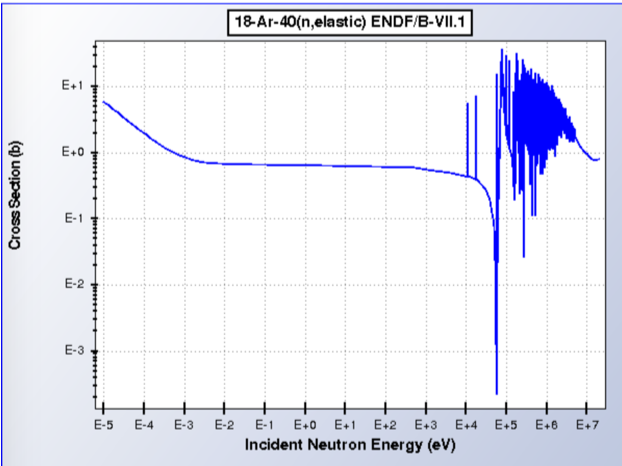
\includegraphics[width=0.4\linewidth]{Figures/Ar40xsec.png}
%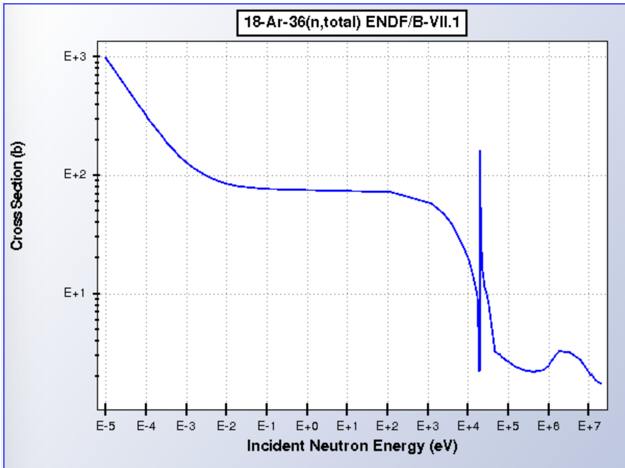
\includegraphics[width=0.4\linewidth]{Figures/Ar36xsec.png}
%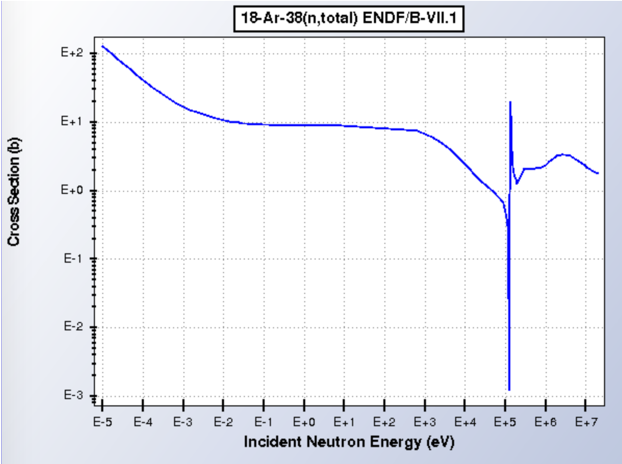
\includegraphics[width=0.4\linewidth]{Figures/Ar38xsec.png}
%\caption{Elastic scattering cross sections on 40-Ar (top left), 36-Ar (top right), and 38-Ar (bottom). From ENDF/B-VII.1~\cite{ref:ENDF}. The large anti-resonance at $57\; keV$ in 40-Ar can be clearly seen.
%{\bf NOTE: PUT IN PLOTS FOR ELASTIC}
%}
%\label{fig:Arxsec}
%\end{center}
%\end{figure}


%\begin{figure}[h]
%\begin{center}
%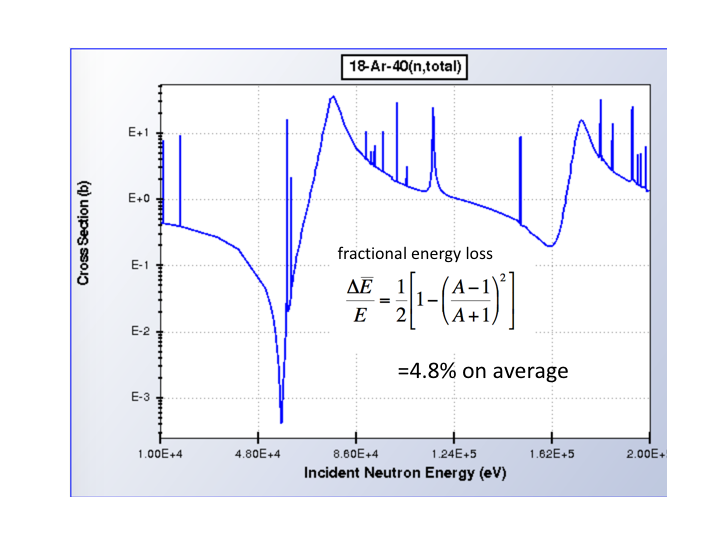
\includegraphics[width=0.75\linewidth]{Figures/Ar40Xsec2.png}
%\caption{Total scattering cross sections on 40-Ar in the range $10-200\; keV$~\cite{ref:ENDF}}
%\label{fig:Arxsec2}
%\end{center}
%\end{figure}

\dword{lar} is nearly transparent to neutrons with an energy near or at \SI{57}{\keV} due to an anti-resonance in the cross-section caused by the destructive interference between two high level states of the \argon40 nucleus (see Figure~\ref{fig:PNS_xsections_v2}). The cross-section at the anti-resonance dip is approximately \SI{10}{\keV} wide, and at the bottom, the cross section of \SI{1.6e-4}{\barn} indicates an elastic scattering length of more than \SI{2000}{\m}. %Of course, natural 

\begin{dunefigure}[x-sections enabling the \dword{pns} concept]{fig:PNS_xsections_v2}
{Illustration of interference anti-resonance dips in the cross-section of \isotope{Fe}{56}, \isotope{Si}{28}, \isotope{S}{32}, and \isotope{Ar}{40}. Elastic scattering cross-section data is obtained from ENDF VIII.0.}
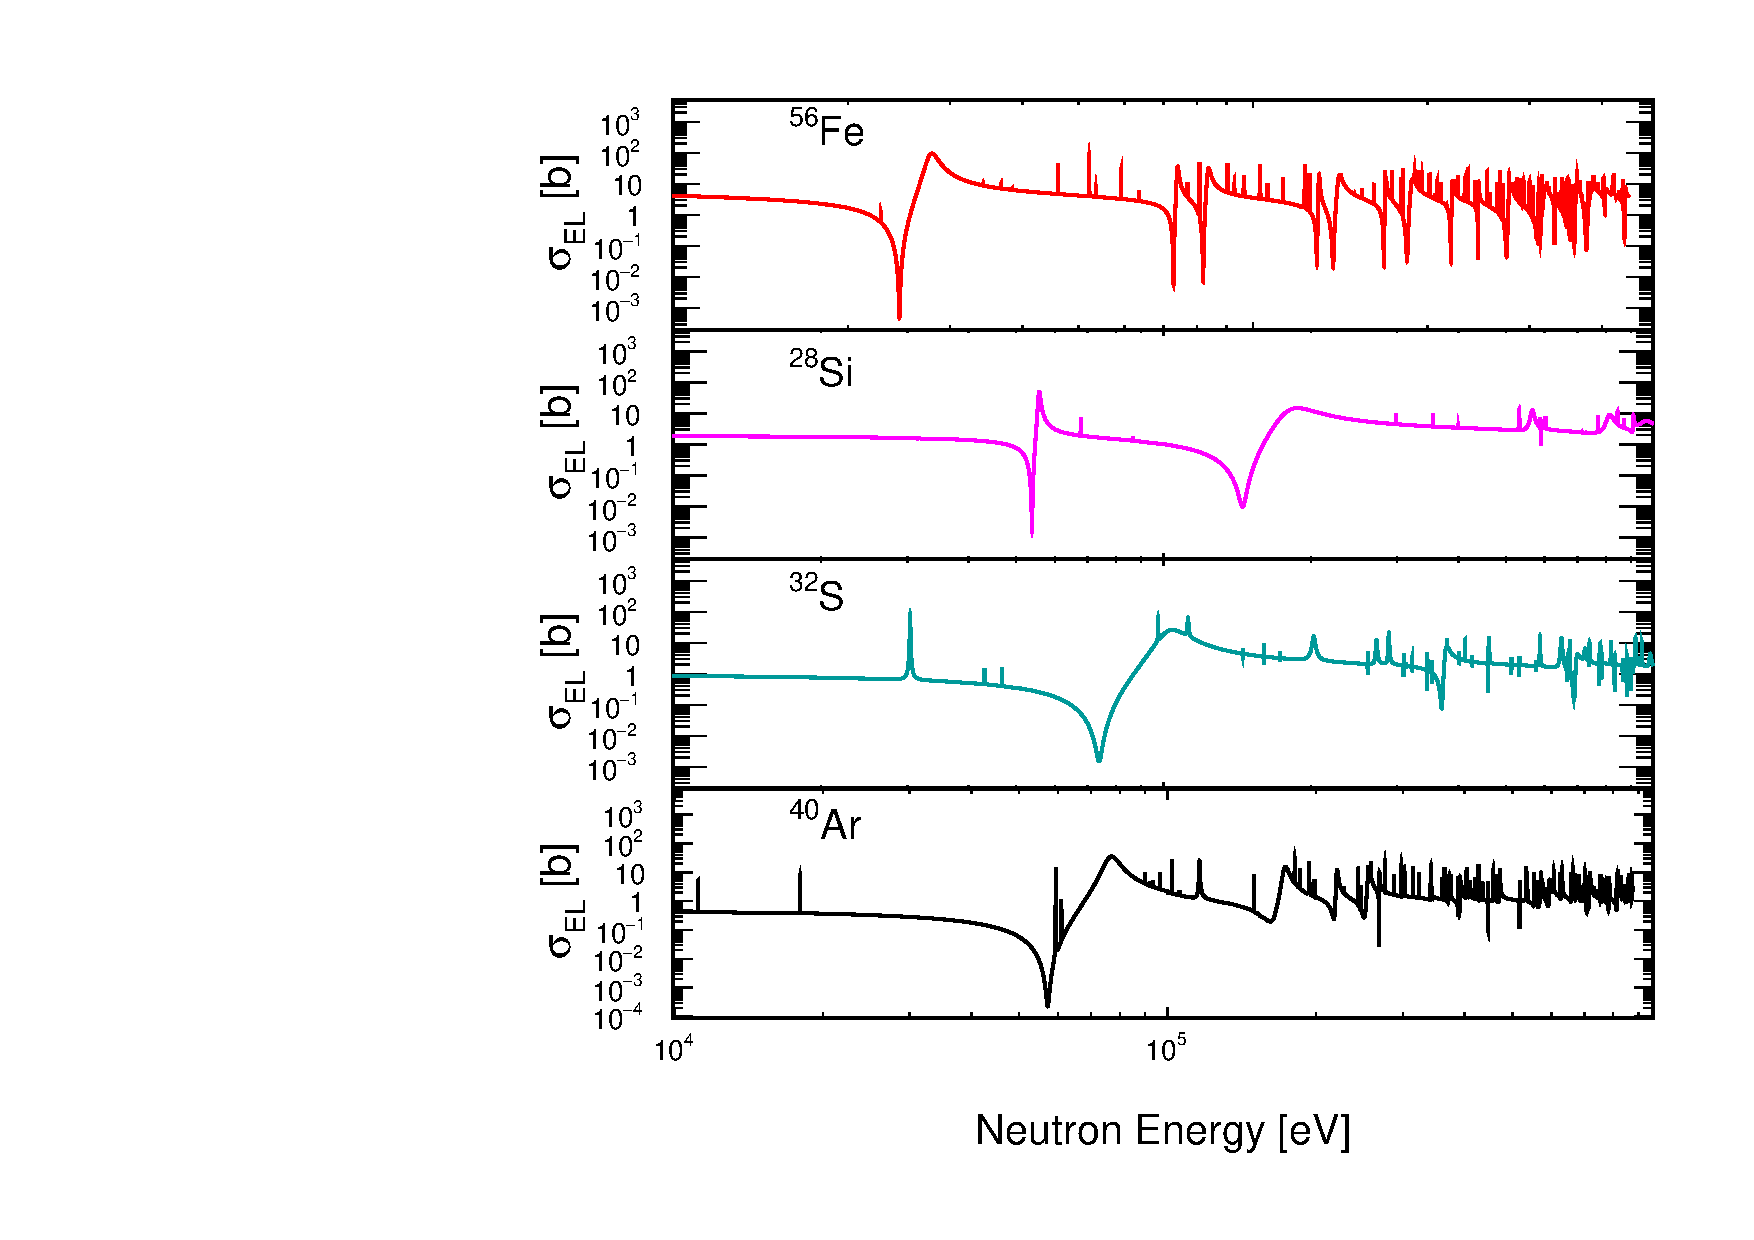
\includegraphics[width=10cm]{graphics/PNS_xsection.pdf}
\end{dunefigure}

Natural argon has three major isotopes: \isotope{Ar}{36} (\SI{0.3336}{\%}), \isotope{Ar}{38} (\SI{0.0834}{\%}), and \isotope{Ar}{40} (\SI{99.6035}{\%}) each with a slightly different anti-resonance. The average elastic scattering length of the \SI{57}{\keV} neutrons in natural liquid argon is approximately \SI{30}{\m}, dominated by \isotope{Ar}{36}.

The neutrons at the anti-resonance energy could be injected into \dword{lar} in the \dword{tpc}, provided no materials (e.g., hydrocarbons) block the path. Those neutrons that do scatter lose energy, leave the anti-resonance, quickly slow down, and are captured. Each capture releases exactly the binding energy difference between \isotope{Ar}{40} and \isotope{Ar}{41}, approximately \SI{6.1}{\MeV}, in the form of $\gamma$ rays.  As described below, using a {\it DD} generator (where {\it DD} stands for Deuterium-Deuterium), a triggered pulse of neutrons can be generated outside the \dword{tpc} and then injected via a dedicated opening in the insulation into the liquid argon, where it spreads through the \SI{60}{\m} volume of the detector to produce \SI{6.1}{\MeV} energy depositions. \fixme{Should DD be included among the dwords?}
%Using this method, the calibration procedure would be quick (likely a few hours depending on the neutron yield of the DD generator), and there is no need to manufacture short-lived isotopes at an external facility.

The neutron capture cross-section and the $\gamma$ spectrum have been measured and characterized. Recently, the ACED \fixme{This abbreviation must be defined the first time it is used and included in the general glossary. In fact, this whole sentence has quite a few abbreviations that should be either in the glossary or not used at all.} collaboration performed a neutron capture experiment using  the Detector  for Advanced  Neutron  Capture  Experiments  at DANCE (ACED)  at the  Los  Alamos  Neutron  Science  Center  (LANSCE). The result of the neutron capture cross-section was published~\cite{Fischer:2019qfr} and will be used to prepare a database for the neutron capture studies. The data analysis of the energy spectrum of correlated gamma cascades from neutron captures is underway and will be published soon. Figure~\ref{fig:PNS_gamma_ACED_v2} shows an example of the energy spectra of individual gamma clusters measured by ACED. The gamma energy spectrum and the branching ratios in ENDF \fixme{Another undefined abbreviation that is not in the glossary.} library will be updated with the ACED results. 

%aced replaced with Fischer:2019qfr
\begin{dunefigure}[Neutron capture gamma spectrum measured by ACED]{fig:PNS_gamma_ACED_v2}
{Energy spectra of individual gamma clusters measured by ACED. Only events detected in the 0.02-0.04 eV neutron energy window are selected.}
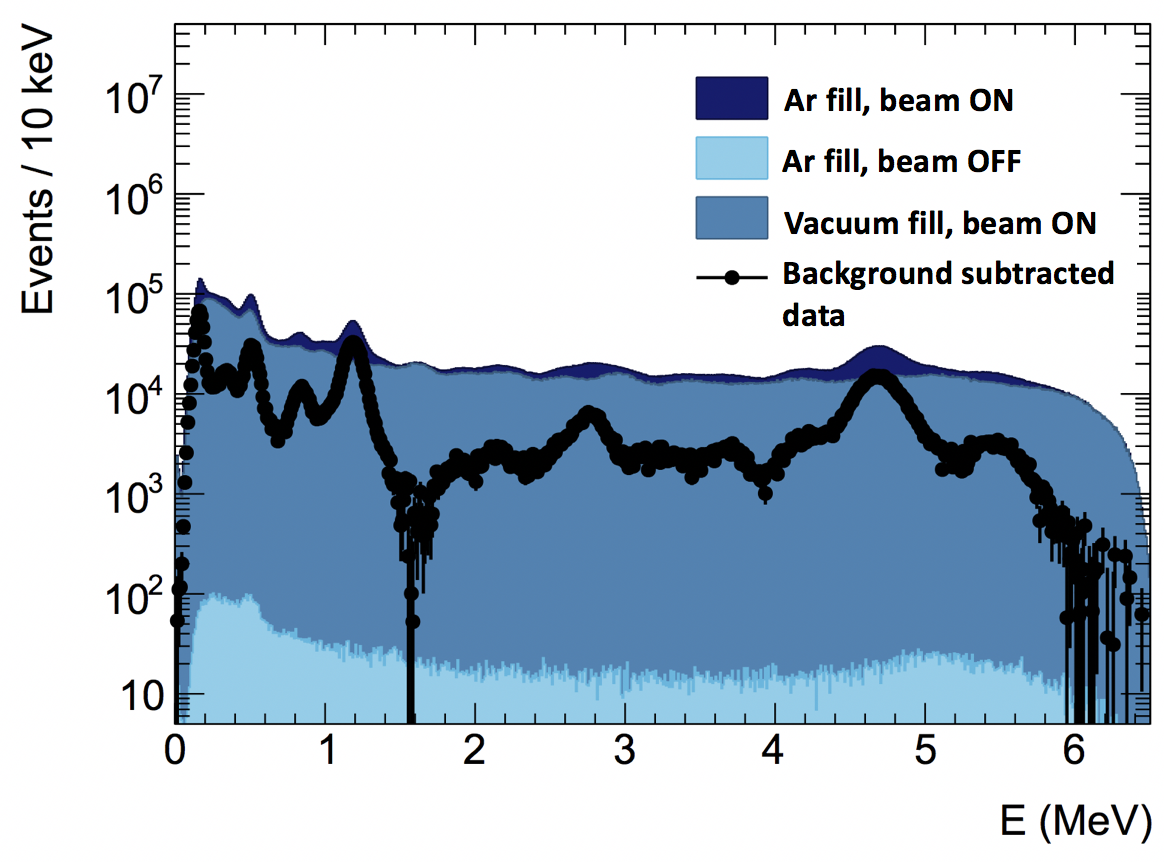
\includegraphics[width=10cm]{graphics/PNS_gamma_ACED_v2.png}
%graphics/PNS_gamma_spectrum_ACED.png}
\end{dunefigure}

%{\it Mention Test at LANSCE and its role?}

%%%%%%%%%%%%%%%%%%%%%%%%%%%%
\subsubsection{Design}
\label{sec:sp-calib-sys-pns-des}

The basic design concept of such a \dword{pns} was successfully used for Boron neutron capture therapy~\cite{bib:Koivunoro2004}. Figure~\ref{fig:PNS_Moderator} shows the design of the \dword{pns} system used for energy calibration. The system will consist of four main components: a $DD$ \fixme{DD is also in italics. Those should be removed once DD is in the glossary.} generator, an energy moderator reducing the energy of the $DD$ neutrons down to the desired level, shielding materials, and a neutron monitor to confirm neutron flux and safe operation. 

\begin{dunefigure}[Conceptual design of the \dlong{pns}]{fig:PNS_Moderator}
{Conceptual design of the \dlong{pns}. The whole device is placed outside the \dword{tpc} volume on top of the cryostat.}
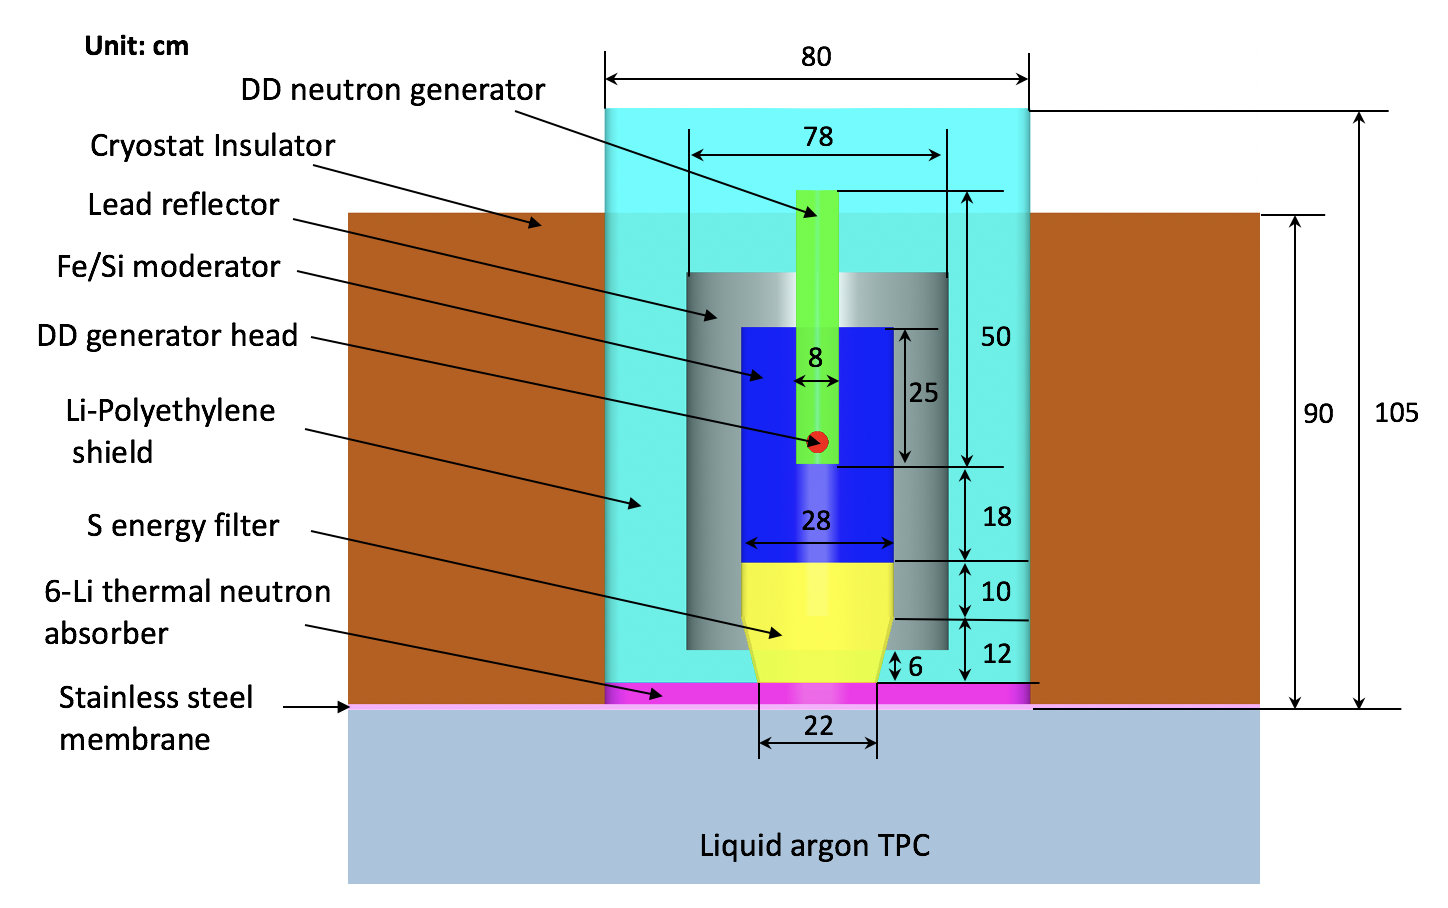
\includegraphics[width=12cm]{PNS_Moderator.png}
\end{dunefigure}



{\bf DD generator source:} \fixme{This does not appear to be consistent with other similar constructions in the document. I don't know that it matters, but I thought I'd better point it out.} $DD$ generators are commercial devices that can be readily obtained from several vendors at a cost of approximately \$\num{125000} each, which includes all control electronics. The pulse width is adjustable and can be delivered from approximately \SIrange{10}{1000}{\micro\s} (which affects the total output). 

{\bf Moderator:}  A feasible moderator has been designed using a layered Moderator~(Fe or Si)-Filter~(S)-Absorber~(Li) %layered 
configuration. The \SI{2.5}{\MeV} neutrons from the $DD$ generator are slowed down to less than \SI{1}{\MeV} by the energy moderator. Natural iron and silicon are efficient moderators for this purpose. Then an energy filter made of sulfur powder further selects the neutrons with the desired anti-resonance energy.
The neutron anti-resonance energy in \isotope{S}{32} is \SI{73}{\keV}, right above the \SI{57}{\keV} anti-resonance energy in \argon40. The neutrons at this energy lose approximately \SI{3.0}{\keV} per elastic scattering length. After a few elastic scattering interactions, most of the \SI{73}{\keV} neutrons selected by the sulfur filter will fall into the \SI{57}{\keV} anti-resonance energy region in \dword{lar}. These materials require no cooling or special handling. Finally, a thermal absorbing volume of Lithium is placed at the entry to the argon pool to capture any neutrons that may have fallen below the \SI{57}{\keV} threshold. The reflecting volume is added around the $DD$ generator and the neutron moderator to increase downward neutron flux. 

{\bf Shielding:} The source will be encased in shielding. The goal of the shield is to block both scattered neutrons and gammas produced in the source. Lithium-Polyethylene (\SI{7.5}{\%}) is the material chosen for the neutron shield because it is rich in hydrogen and lithium atoms, which yield a high neutron absorption cross section. Lithium-Polyethylene is also light weight, commercially available, and relatively inexpensive. The energy spectrum entering the shield has several peaks between \SI{0.5}{\MeV} and \SI{1.5}{\MeV}, and one major spike at \SI{2.2}{\MeV}. The shield can effectively block the lower energy peaks but can only degrade the intensity of the \SI{2.2}{\MeV} because \SI{2.2}{\MeV} gammas are a characteristic signature for neutron captures on hydrogen. A safe thickness of the lithium-polyethylene shield must be found, one that can degrade the dose of \SI{2.2}{\MeV} gammas to safe levels. The dose of radiation from \SI{2.2}{\MeV} gammas was calculated assuming a person standing \SI{1}{\m} away. Simulation indicates that a shield with \SI{12}{\cm} thick Lithium-Polyethylene satisfies basic safety requirements. 

{\bf Neutron Monitor:} The system needs a monitoring system to confirm the source is operating as expected.  A neutron monitoring detector consisting of an Eljen EJ-420 coupled to an ADIT L51B16S \num{2}-inch \dword{pmt} will be placed just outside the moderating material surrounding the $DD$ generator and will be read out with a CAEN waveform digitizer with neutron/$\gamma$ pulse-shape discriminating firmware. The monitoring detector will provide relative flux information to the calibration users and will ensure that the intensity of the source is constant, thereby allowing a comparison of data taking at different times.  A small collimator will be placed in front of the neutron detector, inside the shielding material of the $DD$ source. The collimator dimensions and material specifications (likely a combination of iron, lead, and polyethylene) will be optimized from Monte Carlo simulations.

\begin{dunefigure}[Two designs for the \dlong{pns}]{fig:PNS_Two_Designs}
{Two designs being developed for the \dlong{pns}. Design A: Large format neutron source deployed in dedicated neutron injection ports or above/inside the human access ports; Design B: Small format neutron source deployed inside a standard feedthrough port with \SI{25}{\cm} outer diameter.}
%\todo{SG to Jingbo: I have updated the caption for Figure 1.15, please check}
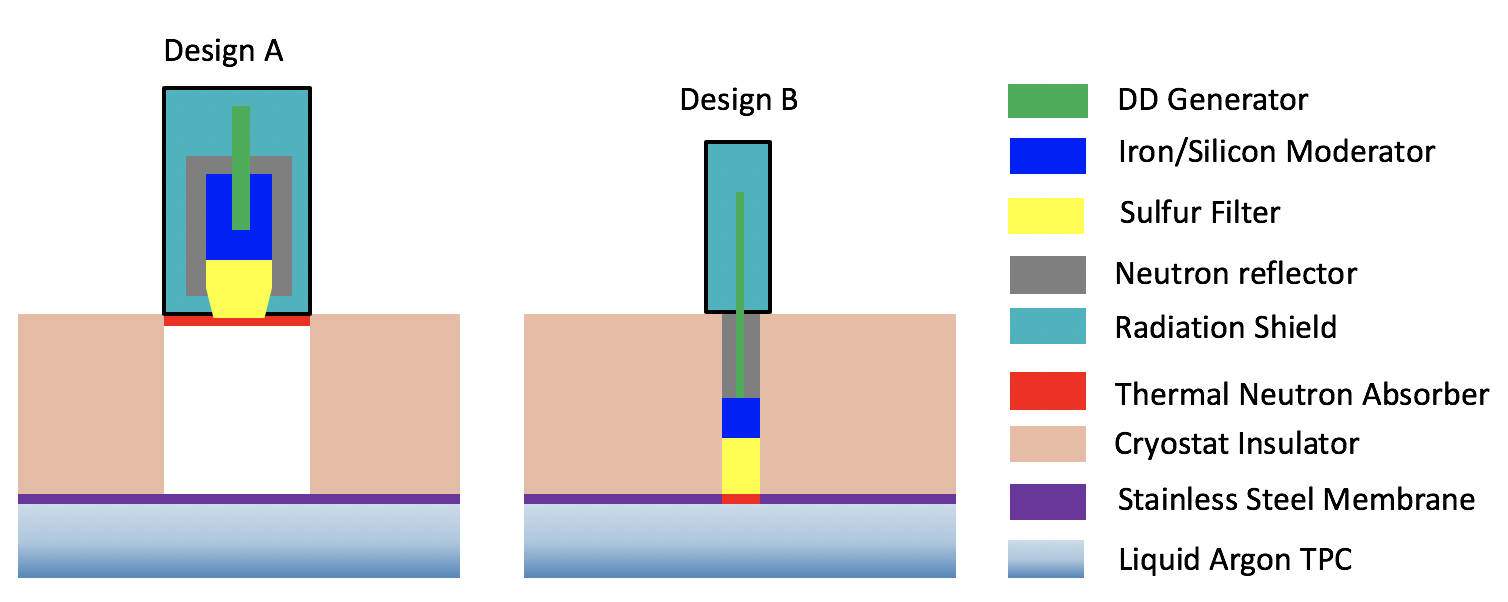
\includegraphics[width=16cm]{PNS_Two_Designs.png}
\end{dunefigure}

Based on the general concept, two different designs were studied with GEANT4 simulation. Figure~\ref{fig:PNS_Two_Designs} shows a conceptual layout of the neutron injection system. %\todo{For v2, confirm updated figure; minor error in current one.}

\begin{itemize}
\item {\it Design A: Large format Moderator:} \\
The neutron source is approximately \SI{0.8}{\m} wide and \SI{1}{\m} high. It would sit above the cryostat insulator. Beneath the neutron source, a cylinder insulator volume more than \SI{50}{\cm} in diameter must be removed to allow the neutrons to enter the cryostat. Such an interface is provided by the human access ports near the end-walls of the detector; Figure~\ref{fig:manhole2} shows a picture of this for \dword{pdsp}. The top flange is sealed, and the neutron source sits on top 
%(Design A), 
providing heat insulation. The neutron source weighs approximately \SI{1.6}{\tonne} and will hang on the I-beam support structure. This design allows the neutron source to be permanently deployed. GEANT4 simulation has shown that \SI{0.13}{\%} of the neutrons generated by the $DD$ generator should be captured inside the \dword{lar} \dword{tpc}. The neutron source may also be placed inside the human access ports, which would allow a \num{6}-fold increase of the neutron flux, but this would require modifying the interface flange. This is currently being investigated.
% JW: I think It doesn't harm to mention that the neutron source could be placed inside the manhole. My recent simulation is based on this configuration.

%\item \fixme{KM: I do not think this is possible for quite a few reasons-- heat loss and also cost of adjusting this. Remnoving this for now.} Design B: Large format Moderator; no insulation between Moderator and cryostat membrane The design of the the neutron source itself would be same as Design A. The only difference is that the neutron source will be placed inside a hole on the cryostat insulator. The cryostat will be kept closed, but there is no vacuum insulation between the neutron moderator and the stainless steel membrane. As the neutron source is closer to the liquid argon cryostat, the neutron flux is expected to be a factor of 10 higher than that of Design A. However, the neutron source must be removed and the insulator has to be recovered after the calibration run. 
\item {\it Design B: Small format Moderator:}\\
%no insulation between Moderator liquid argon. 
%An alternative method for delivering the neutrons is to use the existing calibration feedthroughs. In the current cryostat design, \num{20} calibration feedthroughs with a \SI{20}{\cm} inner diameter will be available on top of the cryostat. 
%\todo{SG: Jingbo, check the modification for this. Although we will aim for our ideal ports, it is good to have small format moderator so we have the flexibility to deploy where we think coverage is needed}
The neutron source can be designed with an ultra-thin $DD$ generator that fits a standard-sized feedthrough (\SI{25}{\cm} outer diameter), which permits deploying the neutron source using existing feedthroughs (e.g., instrumentation or other calibration ports). The problem is that the feedthrough has no space for the shielding materials to fit inside, so additional shielding must be placed around the feedthrough. The weight of this compact neutron source will be approximately \SI{140}{\kg}, so mounting would be simpler than in Design A. The effective neutron flux should be similar to Design A. 
\end{itemize}

\begin{dunefigure}[Flange for human access port on \dword{pdsp}]{fig:manhole2}
{Flange for human access port on \dword{pdsp} and support structure (red frame).}
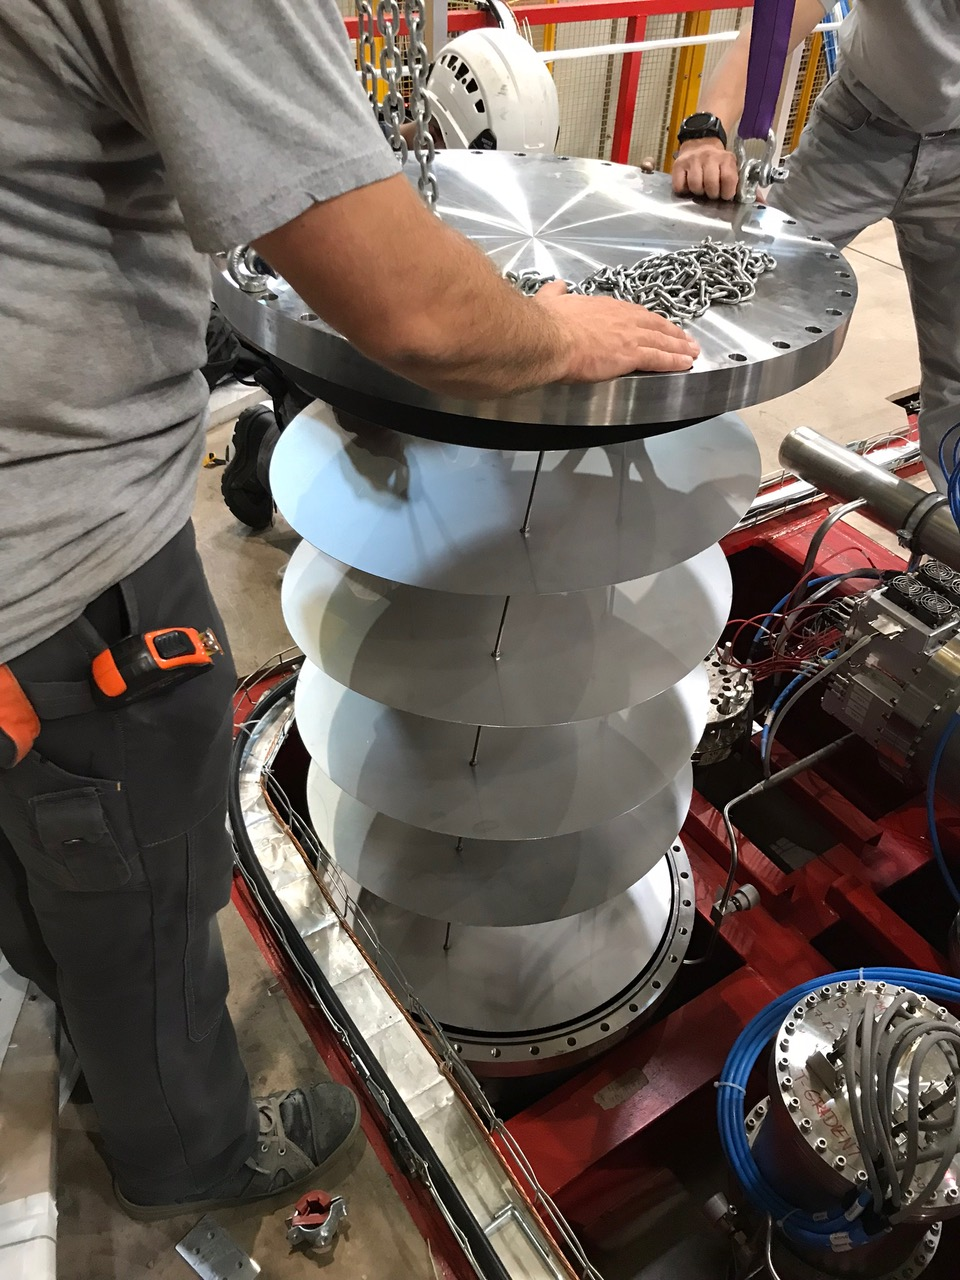
\includegraphics[width=6cm]{manhole2.jpg}
\end{dunefigure}

\begin{dunefigure}[Pulsed neutron system neutron capture positions inside a \dword{dune}-sized TPC]{fig:PNS_NcapPosition}
{Neutron capture positions inside a \dword{dune}-sized \dword{tpc}. L=\SI{60}{\m} (along $z$ axis, horizontally parallel to the beam direction), W=\SI{14.5}{\m} (along $x$ axis, horizontally perpendicular to the beam direction), H=\SI{10}{\m} (along $y$ axis, vertically perpendicular to the beam direction). The neutron moderator is based on Design A, but the entire source is placed inside the injection port central to the cryostat. \num{1e6} DD generator neutrons with \SI{2.5}{\MeV} energy were simulated in the moderator and propagated inside the \dword{lar} \dword{tpc}. Left: Top view of neutron capture positions. Right: Side view of neutron capture positions.}
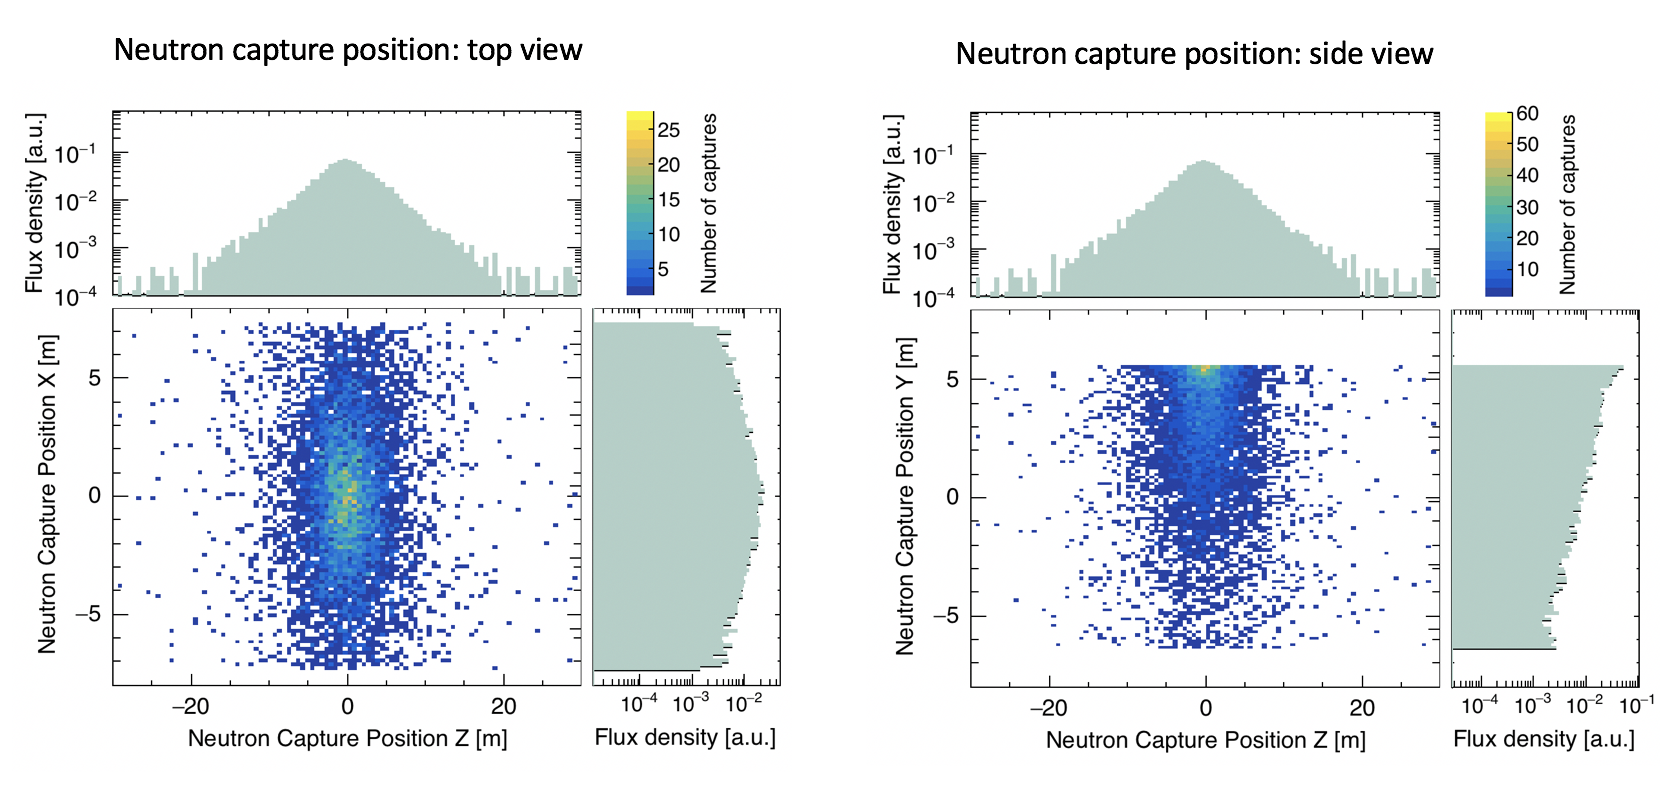
\includegraphics[width=18cm]{PNS_NcapPosition.png}
%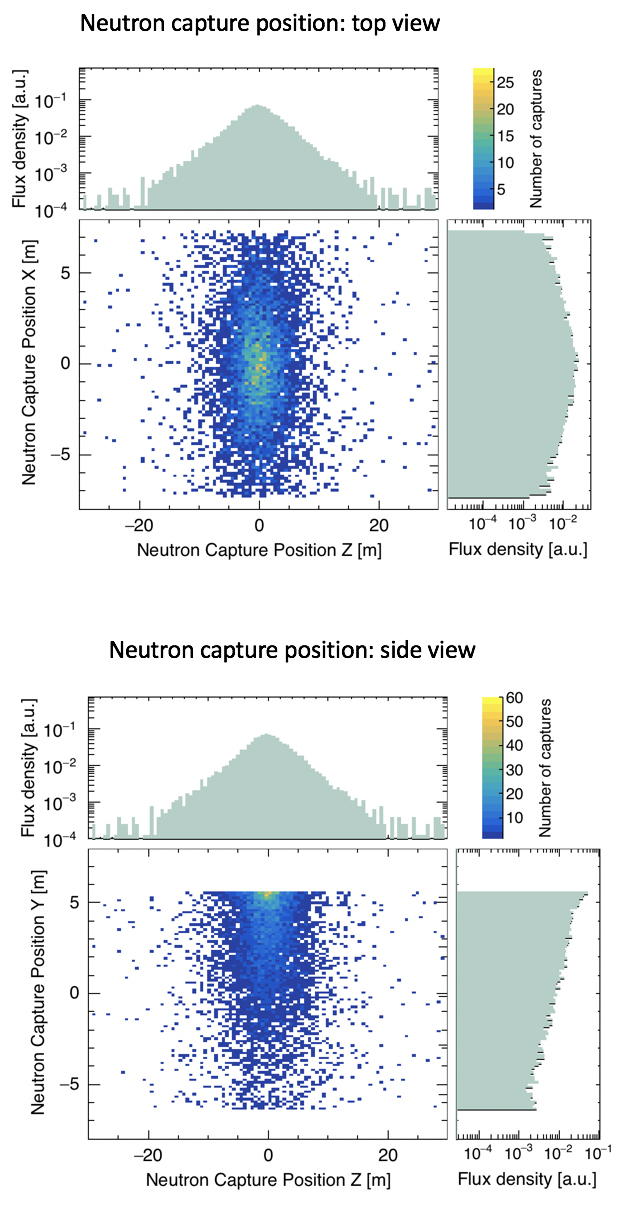
\includegraphics[width=10cm]{PNS_NcapPosition_v2.png}
\end{dunefigure}

%\fixme{SG to Jingbo: Below paragraph is modified. take a look}

The two designs were simulated in GEANT4. Figure~\ref{fig:PNS_NcapPosition} shows the position distribution of the neutron captures. In the simulation, the \dword{pns} is placed on top of the cryostat and is the same size as the \dword{dune} \SI{10}{\kton} \dword{tpc}.  Initial simulation results indicate that one \dword{pns} could cover half the \dword{tpc} volume, so two identical neutron sources, each located at the center of each half of the cryostat
%each central to half the cryostat top,  %\todo{SG: I assume this is with design A, right? if so, mention which design}
would illuminate the whole \dword{tpc} volume of the \dword{dune} \dword{fd} for both designs. This will require two ports, each at 1/4 of the module length (along the beam direction) from each side. This is currently the plan, but the exact locations of the ports are not yet final.
%However, this would require opening two additional neutron injection ports which are not included in the current cryostat design \footnote{Ideally, opening two identical neutron injection ports for each \SI{10}{\kton} TPC would make full use of the neutron source. The possibility requires further discussion with the cryostat engineers.}. 
Alternatively, two large format neutron sources (Design A) could be permanently deployed in the human access ports at the corners of the cryostat. One concern in this approach is that the neutrons scattered from the \dword{lar} volume from the human access ports may not reach the center of the \dword{tpc}. This can be mitigated by using a small format neutron source (Design B) deployed on top of the cryostat at the center using the other available feedthroughs. %could be used to complement the coverage of the large format sources. 
In either case, the source will be injected from the top, and neutrons must penetrate the \dword{crp} readout planes, which can reduce the neutron flux going into the \dword{lar}. %\todo{SG to Jingbo: I added the previous sentence, take a look} 
This is currently being investigated.
Figure~\ref{fig:PNS_Energy_Moderator} shows the energy spectrum of the neutrons moderated and injected into the \dword{lartpc} based on Design A.
% This figure is based on Design A moderator placed inside the manhole. We can still use this figure, because the energy spectrum shape should be same. Only the flux will be a factor of 6 lower
%The neutron energy is moderated from 2.5 MeV to below 100 keV.  



\begin{dunefigure}[Energy of moderated neutrons produced by the \dlong{pns}]{fig:PNS_Energy_Moderator}
{Energy of moderated neutrons produced by the \dlong{pns}. Simulation is based on Design A. The total number of initial DD generator neutrons is \num{1e6}. }
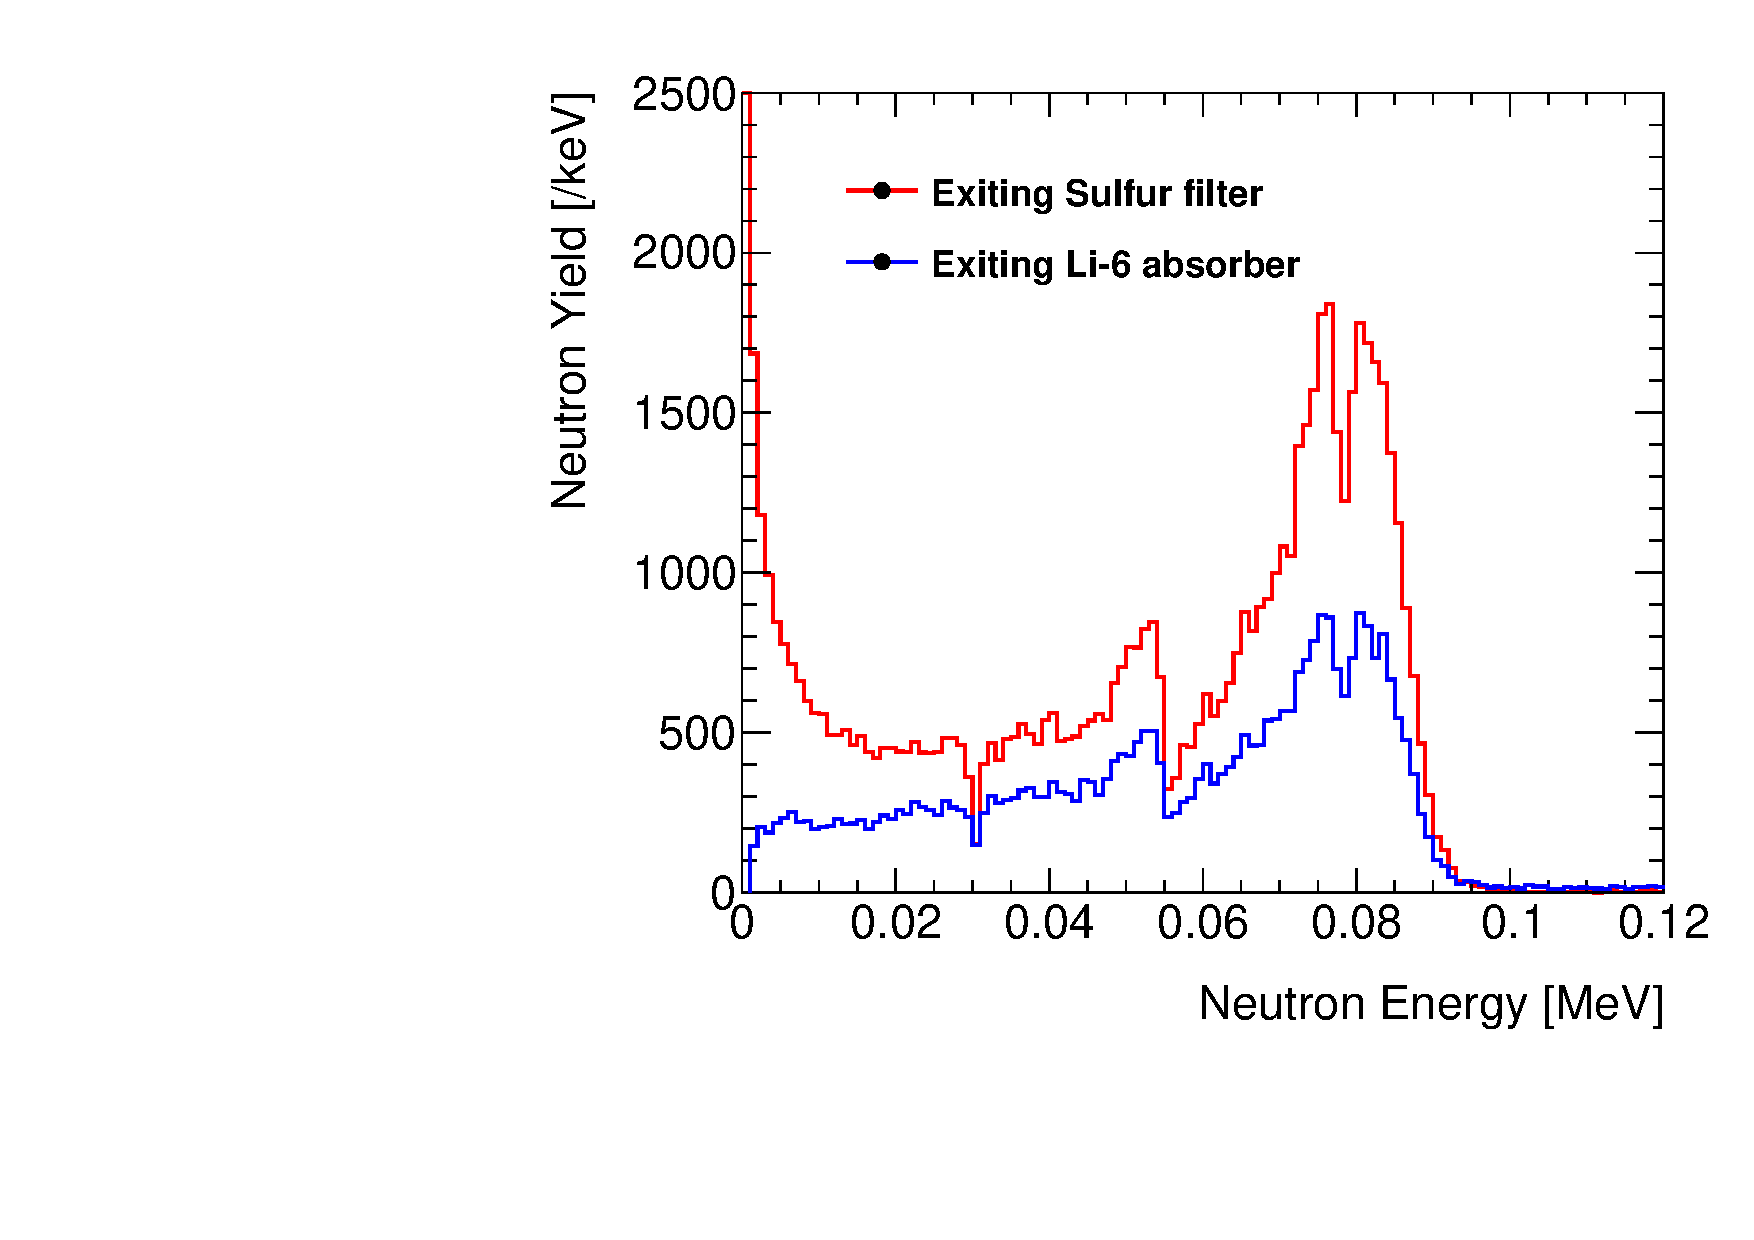
\includegraphics[width=10cm]{PNS_Energy_Moderator.pdf}
\end{dunefigure}

The system should have a long operating lifetime, but because the \dword{pns} system sits on top of the cryostat, with no opening to the \dword{lar}, the system can be replaced if it fails using only crane support.


%%%%%%%%%%%%%%%%%%%%%%%%%%%%
\subsubsection{Measurement Program}
\label{sec:sp-calib-sys-pns-meas}

The \SI{6.1}{\MeV} $\gamma$ cascade will provide a uniform signal for neutron capture, part of the supernova signal. The source may also be used to determine the relative efficiency across the detector for neutron capture,as well as measure energy resolution and energy scale spatially and temporally. Simulation studies are currently underway.
%and for the second draft, we plan to include a first round of simulation results.

%\todo{Simulation studies are underway but changing rapidly. for v2 we will include a first round of studies.}

The first goal of the simulation is to provide the expected distribution of signals, with a normalization given by the pulse width of \dword{pns} operation, and the energy and angular correlated distribution of neutrons, depending on the source filter and shield design, that can also be used to optimize the calibration strategy.
%. It will be used to optimize the calibration strategy too. 
The calibration can be done in two modes: first, a short \dword{pns} pulse can provide isolated neutron captures closer to the entrance path; and then a longer \dword{pns} pulse, for which the same region is saturated, but with isolated neutrons captures obtained in the full volume.

By using an external trigger coupled to the \dword{pns} operation and running the usual trigger algorithms in parallel, the calibration will provide the efficiency of the trigger and \dword{daq} systems as a function of total fluxes. Changing the pulse width can result in 
%resulting on 
higher or lower detector activity. The source will be used for \dword{snb} calibration to test
%, in the sense of testing 
the capabilities of triggering for low energy signals, but also 
%of identifying 
to identify them in different pile-up conditions.
Transmitting the global timing from the external \dword{pns} trigger to the \dword{daq} provides a strong constraint on the initial timing for the \dword{tpc}
%Time Projection Chamber 
because the neutron capture times are approximately \SI{0.15}{\milli\s}, much lower than typical drift time scale for the \dword{tpc}. The photon detectors, with resolutions of \SI{100}{\nano\s}, can discriminate between different neutron captures. The calibration will measure the efficiency of the \dword{pds} response for low energy events, depending on the distance due to the Rayleigh scattering in Argon \fixme{Is this the liquid argon? If so, the dword should be used. Otherwise, in every other place in the manuscript, the scientific abbreviation has been used.}. We will then study using the \dword{pds} time information to improve the position reconstruction of \dword{tpc} signals. Without the \dword{pds} system, the global timing from the \dword{pns} translates to an uncertainty of approximately \SI{10}{\cm}.

Individual event positions can be translated into response maps for both the photon detectors and the \dword{lartpc} to standard candles of \SI{6.1}{\MeV} electromagnetic depositions. When the cascades can be more precisely reconstructed, individual gammas within the cascades can be identified, setting an even lower standard candle, close to the solar electron-neutrino thresholds. Comparing the collected charge for equal energy signals at difference distances from the \dword{tpc} gives a measurement of the electron lifetime, the main response parameter. High \dword{pns} flux runs can generate momentary local space charge effects, in the
%top parts 
upper regions of the detector that must be characterized; low flux runs should be done beforehand to ensure 
%usual 
expected space charge distributions.
The global simulation will be tested in the (smaller scale) \dword{protodune} detectors. The neutron mean free path will be larger than the \dword{protodune} size, and so 
%there will be more 
external events and interactions with materials of the \dword{pds}, \dword{crp}, and \dword{hv} systems will be more prominent. These effects must be simulated.

%Notice 
Note that captures of external background neutrons entering the active volume is a main background for low energy physics;  a comparison of the simulation of the \dword{pns} events with external neutron backgrounds will be interesting, as will a comparison of supernova and solar neutrino signals. \fixme{Please check the preceding sentence. It was unclear, but I'm not sure I got it right.} For the high energy beam events, the number and energy distributions of neutrons depend on the interaction and are significantly different for neutrinos and anti-neutrinos. Measuring the number and distance of neutron captures around the main hadronic cascades can thus help in identifying which extra proton scattering signals to associate to the hadronic cascades or in a statistical correction to the energy reconstruction of the neutrino and anti-neutrino events. \fixme{I'm not sure about the clarity of this final sentence either.}





%%%%%%%%%%%%%%%%%%%%%%%%%%%%%%%%%%%%%%%%%%%%%%%%%%%%%%%

%\subsection{Proposed System: Radioactive Source Calibration System}
%\label{sec:dp-calib-sys-rs}

% \fixme{Call it "deployment" or "calibration" system?}
%%%%%%%%%%%%%%%%%%%%%%%%%%%%%%%%

%\fixme{KM: done for now, but am not satisfied with the end of it-- Juergen did not provide measurements! SG/JM: please briefly check to make sure it is coherent? SG: done. Sent an email to Juergen with some items to be addressed.}

%\subsubsection{Physics Motivation}

Radioactive source deployment provides an in-situ source of physics signals at a known location and with a known activity that can be chosen such that there is only one calibration event per drift time window. The 
primary
%baseline 
source design probes de-excitation products ($\gamma$-rays) which are directly relevant for detection of supernova neutrinos and \isotope{B}{8}/hep solar neutrinos. The \dlong{rsds} (\dshort{rsds}) is the only calibration system that could probe the detection capability for single isolated solar neutrino events and study how well radiological backgrounds can be suppressed. The trigger efficiency could be studied as a function of threshold. 

Other measurements with the primary source include electro-magnetic (EM) shower characterization for long-baseline $\nu_e$ CC events, electron lifetime and \efield as a function of \dword{detmodule} vertical position, individual light detector response, and determination of radiative components of the Michel electron energy spectrum from muon decays. Aside from the 
%baseline
primary nickel source that produces \SI{9}{\MeV} $\gamma$-rays via the \isotope{Ni}{58}(n,$\gamma$)\isotope{Ni}{59} reaction, other sources could be deployed with the same multi-purpose system, for example an ($\alpha$,$\gamma$)
 %\isotope{Ar}{40}($\alpha$,$\gamma$)\isotope{Ca}{44}
%\fixme{isn't this actually an alpha source?}
%gamma-ray 
source, and \isotope{Cf}{252} and/or AmBe neutron sources that probe the impact of various radiological backgrounds, like radon (causing  ($\alpha,\,\gamma$) events) or radiological neutrons, or simply measure the neutron tagging efficiency, useful for improved calorimetry of beam neutrino interactions. In contrast to the primary %$^{58}$Ni(n,$\gamma$)$^{59}$Ni
nickel source with \SI{9}{\MeV} gamma-rays, the ($\alpha$,$\gamma$) source producing gamma-ray energies around \SI{15}{\MeV} via the
\isotope{Ar}{40}($\alpha$,$\gamma$)\isotope{Ca}{44}
%$^{40}Ar(\alpha,\,\gamma)^{44}$Ca 
reaction could even be deployed outside of the cryostat, to probe the upper visible energy range and trigger efficiency for \isotope{B}{8}/hep solar neutrinos. 

Both the \dshort{rsds} and the \dword{pns} systems are needed to address the integrated response of the detector for low energy physics, especially \dword{snb} and $^{8}B$/hep solar neutrinos. 
The \dword{rsds} primarily probes for trigger efficiency, the \dword{pns} tests mostly for uniformity. Response in argon may change rapidly as a function of photon energy due to underlying nuclear physics mechanisms. A combination of \SI{6}{\MeV} (direct neutron capture response), \SI{9}{\MeV} (from the nickel source),
%(peak visible $\gamma$-energy of interest to \dword{snb} and $^{8}B$/hep solar neutrinos), 
\SI{15}{\MeV} (from the ($\alpha$,$\gamma$) source)
is needed to map the low energy response. In terms of complementarity, radioactive sources provide a known position, known-energy single photon events that could be triggered on, while the pulsed neutron source provides a simple, potentially, non-invasive design with externally triggered multi-photon energy signature which is visible across the entire detector with a known time signature.


%%%%%%%%%%%%%%%%
\subsubsection{Design Considerations}

A composite source can be used that consists of \isotope{Cf}{252}, a strong neutron emitter, and \isotope{Ni}{58}, which, via the \isotope{Ni}{58}(n,$\gamma$)\isotope{Ni}{59} process, converts one of the 
\isotope{Cf}{252} fission neutrons, suitably moderated, to a monoenergetic \SI{9}{\MeV} photon~\cite{Rogers:1996ks}. 
The source is envisaged to be inside a cylindrical moderator with mass of about \SI{15}{\kg} and a diameter of \SI{20}{\cm} such that it can be deployed via the multipurpose instrumentation ports discussed in Section~\ref{sec:dp-calib-cryostat}. The activity of the radioactive source is chosen such that no more than one \SI{9}{\MeV} capture $\gamma$-event occurs during a single drift period. This forms the main requirement for this system as this allows one to use the arrival time of the measured light as a $t_0$ and then measure the average drift time of the corresponding charge signal(s). Table~\ref{tab:fdgen-calib-all-reqs-rsds} lists the full set of requirements for the \dlong{rsds}.

The sources would be deployed outside the \dword{fc} within the cryostat to avoid regions with high \efield{}s, approximately \SI{30}{\cm} from the \dword{fc}. The $\gamma$-ray would need to travel two attenuation lengths (including the \SI{10}{\cm} radius of the source body). Such high $\gamma$-energies are typically only achieved by thermal neutron capture, which invokes a neutron source surrounded by a large amount of moderator, thus driving the size of the source.
%making such an externally deployed (n, $\gamma$) source \SI{20}{\cm}  to \SI{50}{\cm} % large
in diameter. 

For the proposed \dword{rsds} system, ports must be close to the end-walls. An advantage of this system in \dword{dp} is that the source movement is along the drift direction, so several runs can be taken at different positions along the drift coordinate, which is important to check the detector response. %Between \num{4} and \num{10} additional ports should be available for the \dword{pns} system (toward middle of the cryostat) and the proposed \dword{rsds} system (close to the east and west end-walls). 
The exact locations of these additional ports is yet to be finalized.

\begin{dunetable}
[Full specifications for the radioactive source deployment system]
{p{0.45\linewidth}p{0.25\linewidth}p{0.25\linewidth}}
{tab:fdgen-calib-all-reqs-rsds}
{Full list of specifications for radioactive source deployment system.}   
Quantity/Parameter	& Specification	& Goal		 \\ \toprowrule   
%\textbf{Proposed Radioactive Source System}	   &   &  \\ \colhline  
Distance of the source from the field cage & \SI{30}{\cm} & \\ \colhline
Rate of \SI{9}{\MeV} capture $\gamma$-events inside the source (top-level requirement) & < \SI{1}{\k\hertz} & \\ \colhline 
Data volume per \SI{10}{\kt} & \SI{114}{TB\per\year} & \SI{228}{TB\per\year} \\ \colhline 
Longevity	& \dunelifetime			& > \dunelifetime   \\   
%Stability & Match precision requirement at all places/times	&  \\ \colhline  Reliability	& Measurements as needed & Measurements as needed \\ \colhline
\end{dunetable}

%In~\cite{Rogers:1996ks}, %\fixme{This needs to be restated: In Jones [4]... (with Jones being the name of the author).}
%\cite{Triumf:Nickelsource} 
%\todo{SG: reference needs fixing},
A gamma source based on the \isotope{Ni}{58}(n,$\gamma$)\isotope{Ni}{59} reaction, and triggered by an AmBe neutron source, has been successfully built~\cite{Rogers:1996ks}, yielding high $\gamma$-energies of \SI{9}{\MeV}. \dword{dune} %We 
proposes to use a \isotope{Cf}{252} (or AmLi as backup) neutron source with lower neutron energies, which requires less than half of the surrounding moderator, and making the \isotope{Ni}{58} (n, $\gamma$) source only \SI{20}{\cm} or less in diameter. A cryostat feedthrough at either end of the cryostat (east and west sides) outside the \dword{fc} with an outer diameter of \SI{25}{\cm} will be suitable for this. The exact locations of ports is being explored.
%The multipurpose instrumentation feedthroughs at either end of the cryostat are sufficient for this, and have an inner diameter of \SI{25}{\cm}.  
 The moderator material chosen for \dword{dune} is Delrin,\footnote{DuPont\texttrademark Delrin\textregistered, \url{http://www.dupont.com/products-and-services/plastics-polymers-resins/thermoplastics/brands/delrin-acetal-resin.html}.} which has a large enough density to avoid flotation. Further, the end caps of the source
body are round to avoid distorting the \efield and to
eliminate the risk of the source becoming stuck during deployment. 
%JM 19May2019: I commented out the figure and text below since it's for SP only; SG: put it back in since it serves as a nice example for both SP and DP.
Figure~\ref{fig:RadioactiveSource_zm40cm_xp220cm} depicts the primary source design of a cylindrical Delrin moderator \SI{20}{\cm} in diameter and \SI{40}{\cm} high, including half-spheres at either end with
radius of \SI{10}{\cm}, deployed at $z$=\SI{40}{\cm} outside the \dword{fc} and leaving a gap of \SI{30}{\cm} from the \dword{fc}. Deployed along the full vertical height (at each feedthrough location) the 9~MeV $\gamma$-ray source can illuminate the full drift length from bottom cathode to \dword{crp}.

\begin{dunefigure}[Fish-line deployment scheme in \dshort{dune} for an encapsulated radioactive source]
{fig:RadioactiveSource_zm40cm_xp220cm}
{Fish-line deployment scheme in \dword{dune} for a radioactive source encapsulated inside a cylindrical Delrin moderator body \SI{20}{\cm} in diameter and \SI{40}{\cm} high, including half-spheres with a radius of \SI{10}{\cm} at either end. A $^{252}$Cf neutron source and a natural Ni target are sealed inside at the center. The fish-line is deployed \SI{40}{\cm} outside of the \dword{fc}  (depicted here for the \dword{sp} but also valid for \dword{dp}).
%and \SI{220}{\cm} away from the \dword{apa} (red plane).
}
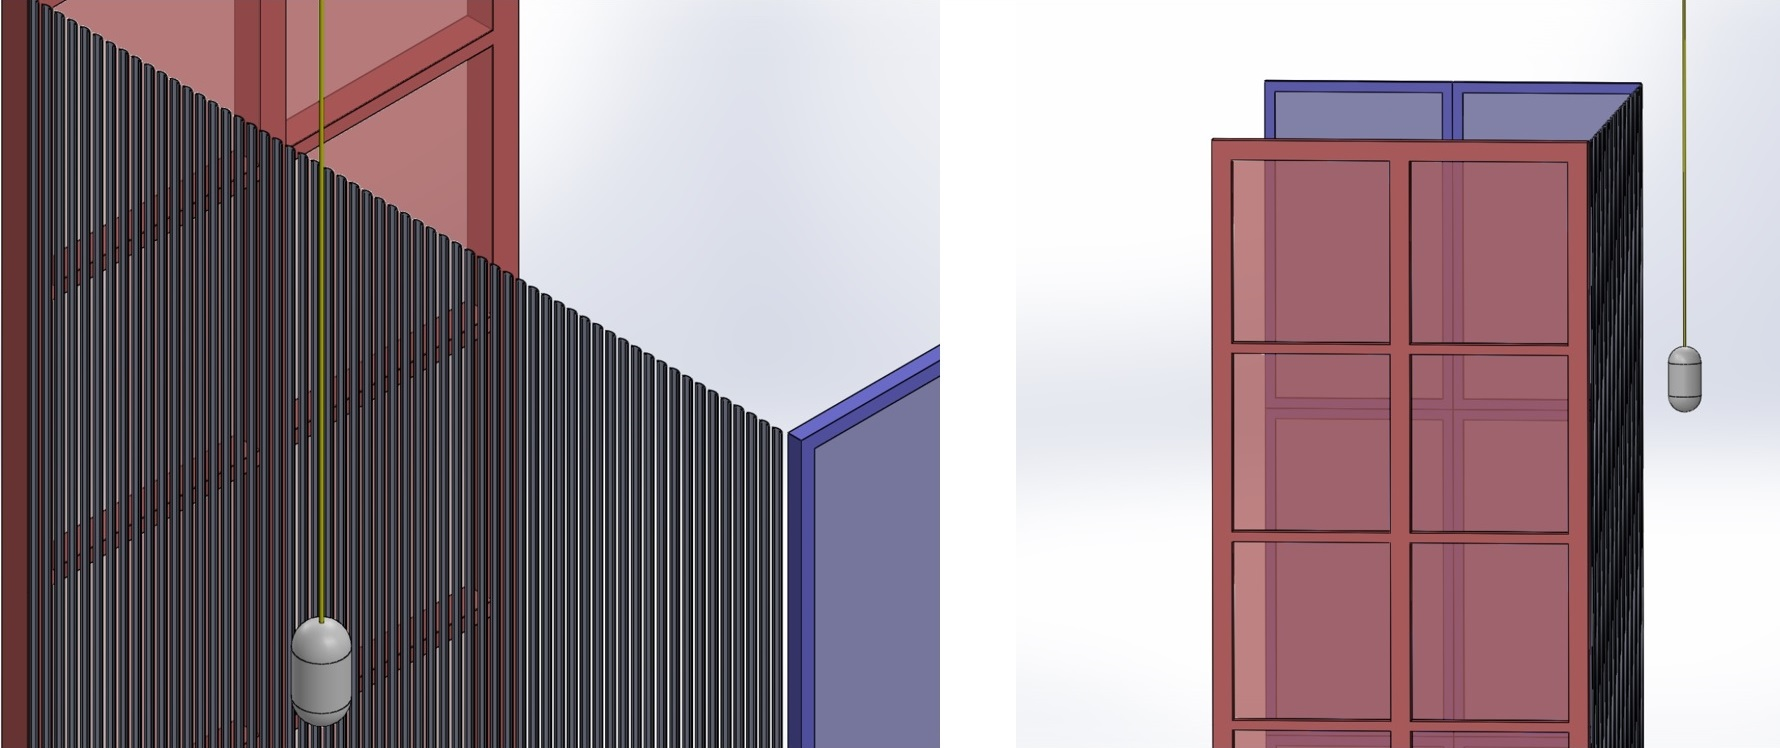
\includegraphics[width=1.0\linewidth]{RadioactiveSource_zm40cm_xp220cm.jpg}
\end{dunefigure}

% Here it is, but I don't have privileges for the bibliography

%@Misc{Triumf:Nickelsource,
%  author =   {J. Rogers, M. Andreaco, C. Moisan},
%  title =    {A $7-9$\,MeV isotropic gamma ray source for detector testing},
%  howpublished = {TRIUMF TRI-PP-96-7},
%  month =    {Apr},
%  year =     {1996},
%}

%\fixme{KM: From Juergen but I think covered by above: The activity of the radioactive source is chosen such that no more than one \SI{9}{\MeV} capture $\gamma$-ray spills into the active \dword{lartpc} region during a single \SI{2.2}{\milli\s} drift period. This allows one to use the arrival time of the measured light as $t_{0}$ and then measure the average drift time of the corresponding charge signal(s). The resulting drift velocity in turn yields the electric field strength, averaged over the variations encountered during the drifting of the charge(s). This can be repeated for each single \SI{9}{\MeV} capture $\gamma$-event that occurs during a \SI{2.2}{\milli\s} drift period and where visible $\gamma$-energy is deposited inside the active volume of the TPC. Pile-up and data read-out considerations restrict the maximally permissible event rate to less than \SI{10}{\hertz} and in turn the \SI{9}{\MeV} capture $\gamma$-rate occurring inside the radioactive source body to less than \SI{140}{\hertz}, given a spill-in efficiency into the active \dword{lar} of about \num{7}\%.}

A successfully employed multipurpose fish-line calibration
system
%~\cite{bib:deKerret2012} \todo{SG: Juergen to provide proper reference. JM: Juergen says there's no alternative public ref.} 
% JM, April 2018: We will not refer to this since the LBNC will not have access to it
%\fixme{need to add reference: "The Double Chooz Near Detector Technical Design Report" 
%Double Chooz Collaboration (H. de Kerret (APC, Paris) et al.) Oct 1, 2012. EDMS ID:I-028812 ; DocDB ID: 3403-V5 Pages 198 - 223
%(Anne can't find proper ref for this)}
for the Double Chooz reactor neutrino experiment has become available 
 %for DUNE 
after the decommissioning of Double Chooz in 2018. The system can be
easily refitted for use in \dword{dune}. The system will be housed inside
a purge-box connected via a neck to a multipurpose
calibration feedthrough 
%\fixme{I note that feedthrough is spelled out in this section of source code while in the rest of the manuscript an abbreviation was used.} 
%\fixme{JM: What abbreviation? In the rest of the Calibration chapter we used feedthrough. }
with a closed gate valve on top of the
cryostat. Before deployment, the source will be gently cooled-down by blowing liquid argon boil-off onto it inside a sealed purge-box. After the source has reached 
%near liquid argon 
near-\dword{lar} temperature, the purge-box will be evacuated by a vacuum pump to remove any residual oxygen and nitrogen which is monitored at the ppm level. Then, the entire purge-box interior is purged with boil-off liquid argon, and the pressure equalized with the gas pressure inside the detector, before the gate-valve is opened and deployments can commence. This procedure ensures that no significant impurities are introduced into the detector during a deployment and that no significant amount of liquid argon is boiled off from the detector. 
%Also, if the source is in close proximity of an \dword{apa} wire frame, lower energetic radiological backgrounds become problematic as the source light and charge yield is reduced exponentially with distance. 

%Deployed near mid-drift (in each TPC module) the \SI{9}{\MeV}
%$\gamma$-ray source can illuminate the full drift length from
%\dword{apa} to \dword{cpa}. 
The sources are retrieved from the
detector after each deployment and stored outside the cryostat following approved safety protocols, and the gate-valves are kept closed after deployment. More details on radiation safety and handling procedures are in Section~\ref{sec:dp-calib-rsds-safety}.

\subsubsection{Development Plan}
The major development plans for the \dword{rsds} include
\begin{itemize}
\item Continued development of relevant simulation tools, including geometry representation of the source deployment system and effects of various radiological contaminants on detector response. 
\item Studies to suppress radiological backgrounds for the calibration source.
\item Simulation studies to understand data and trigger rates.
\item A baseline design source with Delrin moderator, $^{252}$Cf neutron source, and natural nickel target, both sealed inside at the moderator's center.
\item Validation of \SI{9}{\MeV} capture $\gamma$-ray yield of source using spectroscopic measurements with the RABBIT germanium detector at the South Dakota School of Mines and Technology, which has an assay chamber large enough for the bulky moderator; 
%\fixme{Check this please. SG: check what?}
\item Validation with $^{3}$He based hodoscope at South Dakota School of Mines and Technology to ensure that the flux of neutrons escaping the moderator is not an issue; otherwise use lower energetic AmLi neutron source instead and/or more moderator material, and/or different geometric configuration of nickel target; 
\item Test gentle GAr cooling of source and validate material integrity; measure tensile strength of braided SS-304 wire-rope at cryogenic temperatures and ensure a safety factor of one order of magnitude by adjusting number of steel braids and their diameters; validate cryogenic shrinkage of sectional teflon sleeves that enclose the braided steel wire-rope and electrically insulate it from the \dword{fc}; 
\item Validation that anticipated fluid flow in \dword{lar} does not cause oscillations of the source; otherwise design vertical guide wires to be pre-installed during detector installation 
%and that they 
that will keep source stable during deployment along the vertical (drift) axis;
%\item A mechanical test of the Double Chooz fish-line deployment system with both an \dword{lar} and liquid nitrogen mock-up column in the high bay lab at South Dakota School of Mines and Technology. The ultimate test of the system will be done at ProtoDUNE. 
\item Explore other radioactive sources beyond the primary %$^{58}$Ni(n,$\gamma$)$^{59}$Ni 
\SI{9}{\MeV} $\gamma$-ray nickel source, such as the previously mentioned \SI{15}{\MeV} $\gamma$-ray source based on the  $^{40}$Ar($\alpha,\,\gamma$)$^{44}$Ca process with $^{241}$Am as the alpha emitter. This is currently being assembled at SDSMT.
%a non-invasive externally employed 
%with $^{241}$Am that is currently being assembled at SDSMT, and that could probe from the outside of the cryostat the upper visible energy range and trigger efficiency for $^{8}B$/hep solar neutrinos. 
Furthermore, investigate hybrid neutron sources ($^{252}$Cf and AmBe) that emulate the kinetic neutron energy spectrum of radiological neutrons and probe the neutron tagging efficiency.
%, useful for improved calorimetry of beam neutrino interactions and for clarification of impact of radiological neutron backgrounds. 
\end{itemize}

%%%%%%%%%%%%%%%%%%%%%%%%%%%%
\subsubsection{Measurement Program}
\label{sec:dp-calib-sys-src-dep-meas}
%new text from Juergen on DP
The proposed primary 9 MeV single $\gamma$ source could also be used to test the $\gamma$ aspect of the \dword{snb} and $^{8}B$/hep solar neutrino signal 
along the full vertical drift, but only in the \endwall regions of the detector because the detector does not have sufficient space on the long sides of the detector. 
The source may also be used to determine the relative charge and light extraction efficiency in the vertical direction for measuring energy resolution and energy scale. The electron lifetime and the \efield strength can be directly measured with vertical deployments that are not far from the \dwords{pmt} at the bottom, so the instant light signal can still be detected and used as t$_0$. Because of the very long vertical drift in the \dword{dp} detector, the \dword{rsds} should provide the most unambiguous measurement of electron lifetime in the \dword{dp} detector.

%SP text, commented out
%The proposed baseline 9~MeV single $\gamma$ source may also be used to test the $\gamma$ aspect of the \dword{snb} and $^{8}B$/hep solar neutrino signal along the full drift but only in the endwall regions of the detector. The source may also be used to determine the relative charge and light extraction efficiency in the vertical direction for measurements of energy resolution and energy scale. 

%SG: this is repetition
%The \dword{rsds} is the only calibration system that could probe the detection capability for single isolated solar neutrino events and study how well radiological backgrounds can be suppressed. 
%Figure~\ref{fig:rsds-fig1}
%{fig:9MeVgamma_withBG_LArSoft_v08_14_00_hiLY_originCHARGEcollected_TopView}
%depicts in a top view of the detector the simulated charge extraction efficiency for the baseline $^{58}$Ni(n,$\gamma$)$^{59}$Ni 9~MeV $\gamma$-ray source deployed \SI{40}{\cm} outside of the \dword{fc}, near mid-drift i.e., \SI{220}{\cm} away from the \dword{apa} in the $x$ direction, in the presence of expected background before (Fig.~\ref{fig:rsds-fig1}(a)) and after (Fig.~\ref{fig:rsds-fig1}(b)) applying selection cuts. The selection cuts discard each collection wire hit with less than 90~ADCU, limit wire hits to be within the width of the outer \dword{apa}, use induction wire hits to discard collection wire hits occurring further than \SI{2.2}{\m} away from the vertical deployment height, and requiring at least one occurrence per \SI{2.2}{\ms} drift-time window of a simultaneously extracted number of photoelectrons of more than 40~pes (within a \SI{50}{\ns} time window).
%Figure~\ref{fig:rsds-fig1}(b)
%Figure~\ref{fig:9MeVgamma_withBG_LArSoft_v08_14_00_hiLY_originCHARGEcollected_TopView} (b) 
%demonstrates that the selection cuts can reject charge from radiological backgrounds almost entirely, such that almost pure 9~MeV gamma-ray events are selected. Thus, the baseline \dword{rsds} would allow the trigger efficiency for isolated solar neutrino events to be studied, and even its dependence on the applied threshold measured. 

%SG: already stated under physics motivation, no need to repeat
%Moreover, the small electronic pulses from 9~MeV gamma-ray induced charge and light collections can be utilized to better characterize electro-magnetic (EM) showers for long-baseline $\nu_e$ CC events, as well as to determine the radiative components of the Michel electron energy spectrum from muon decays. 
%Further secondary measurements from the baseline 9 MeV gamma-ray source deployment include measuring the electron lifetime and electric field as a function of \dword{detmodule} vertical position, as well as the individual light detector response. 

%Figure~\ref{fig:rsds-fig2}
%{9MeVgamma_withBG_LArSoft_v08_14_00_hiLY_DriftTimesEfield_ChargeSpectrumElectronLifetime_cut} 
%shows exemplary simulated baseline \dword{rsds} measurements of the electric field strength (Fig.~\ref{fig:rsds-fig2}(a)) and of the electron lifetime (Fig.~\ref{fig:rsds-fig2}(b)), each for three different scenarios. The time difference between an extracted number of photoelectrons of more than 40~pes and the recorded hit times on collection wires, passing the selection cuts, defines the plotted drift-times. Precise quantities can be extracted from fitting the measured drift-time distribution to the simulation. For this, the simulated collection wire charge (before selection cuts) is re-weighted with respect to 
%(a) 
%the electric field strength, and 
%(b) 
%the electron lifetime, respectively. After each re-weighting of the simulation the selection cuts are then applied. Figure~\ref{fig:rsds-fig2}(a)
%{9MeVgamma_withBG_LArSoft_v08_14_00_hiLY_DriftTimesEfield_ChargeSpectrumElectronLifetime_cut} (a) 
%illustrates that with this method the electric field strength could be measured at $\sim 1\%$ precision at each vertical deployment position at the endwalls. Likewise, %Figure~\ref{fig:rsds-fig2}(b)
%Figure~\ref{9MeVgamma_withBG_LArSoft_v08_14_00_hiLY_DriftTimesEfield_ChargeSpectrumElectronLifetime_cut} (b) 
%illustrates that the electron lifetime could be measured at few $\%$ precision at each vertical deployment position at the endwalls. 

%Figure~\ref{fig:rsds-fig2}(c)
%{9MeVgamma_withBG_LArSoft_v08_14_00_hiLY_DriftTimesEfield_ChargeSpectrumElectronLifetime_cut} (c) 
%illustrates that with a recorded charge spectrum (after selection cuts) it is not convincingly possible to unambiguously measure both the electron lifetime and the electric field strength. Both parameters for most part simply shift the upper falling edge of the charge spectrum further up or down. However, at each vertical \dword{rsds} deployment position at the endwalls, it is still possible to self-consistently measure both the electron lifetime and the electric field strength at $\sim 1\%$ precision: First, the electric field strength is precisely inferred from the drift-time distribution at each deployment position, second the corresponding electron lifetime is then precisely deduced from the charge distribution by using the measured electric field strength as precise constraint. 

%Figure~\ref{fig:rsds-fig2plus} visualizes the simulated change of individual light detector response as a function of \dword{detmodule} vertical position when the baseline source is deployed at one of the possible endwall locations. The uniformity of the optical detection response can be probed with a full vertical scan. Wrong channel mapping, dead or noisy optical detectors could be easily identified. 

Aside from the primary 
%$^{58}$Ni(n,$\gamma$)$^{59}$Ni 9 MeV $\gamma$-ray source
9 MeV $\gamma$-ray nickel source, other sources could be deployed with the same multi-purpose system, for example a $^{40}$Ar($\alpha,\,\gamma$)$^{44}$Ca gamma-ray source, a $^{252}$Cf and/or AmBe neutron source that probes the impact of various radiological backgrounds, like radon ($\alpha,\,\gamma$) or radiological neutrons, or simply measures neutron tagging efficiency, useful for improving calorimetry of beam neutrino interactions. 
In contrast to the nickel source, the \SI{15}{\MeV} ($\alpha,\,\gamma$) could be deployed outside of the cryostat.
%In contrast to the baseline $^{58}$Ni(n,$\gamma$)$^{59}$Ni source with 9~MeV $\gamma$-rays, an $^{40}Ar(\alpha,\,\gamma)^{44}$Ca source producing $\gamma$-ray energies around 15~MeV could even be deployed outside the cryostat and probe the upper visible energy range and trigger efficiency for $^{8}B$/hep solar neutrinos. 

%Figure~\ref{fig:rsds-fig3}
%{5MeValphaSource_zx_TDR_TopView} 
%shows in a top view of the detector the widely spread interaction locations of about half a dozen $^{40}Ar(\alpha,\,\gamma)^{44}$Ca 15 MeV $\gamma$-ray events in terms of detected light (Fig.~\ref{fig:rsds-fig3}(a)) and  detected charge (Fig.~\ref{fig:rsds-fig3}(b)). These simulation plots depict that 15~MeV $\gamma$-rays can travel \SI{7}{\m} in liquid argon, i.e., about half the width and half the height of the detector. It is therefore possible to deploy such a $^{40}Ar(\alpha,\,\gamma)^{44}$Ca 15~MeV $\gamma$-ray source conveniently and non-invasive from the outside of the cryostat, from each side and from the top (assuming that underneath the cryostat there is no accessible space). This would allow for calibrating large parts of the full detector with this source. 

An external \dword{protodune2} deployment can demonstrate the feasibility of the non-invasive \SI{15}{MeV} \argon40$(\alpha,\,\gamma)^{44}$Ca $\gamma$-ray source despite the lack of overburden to shield cosmic rays. In contrast to cosmic muons, \SI{15}{MeV} $\gamma$-ray induced hit clusters will start inside the detector volume, and are not tracks that begin at the detector edges. Thus, the \dword{rsds} calibration events could therefore be easily selected and the detected charge can be analyzed. The detected light, however, will be obscured from the high light level in each drift period from cosmic muons hitting \dword{protodune}. 

%\begin{dunefigure}[Detected charge from 9 MeV gamma-ray source with radiological backgrounds]
%{fig:9MeVgamma_withBG_LArSoft_v08_14_00_hiLY_originCHARGEcollected_TopView}
%{fig:rsds-fig1}
%{In LArSoft backtracked origins of detected charge (a) without cuts and (b) with selection cuts for a simulated 9~MeV $\gamma$-ray source deployed at $z=$\SI{-40}{\cm} outside of the \dword{fc}, $x=$\SI{220}{\cm} away from the \dword{apa}, and $y=$\SI{300}{\cm} half-height of an upper endwall \dword{apa} with simulated expected radiological background, that gets almost eliminated by selection cuts.}
%\centering
%   (a)
%   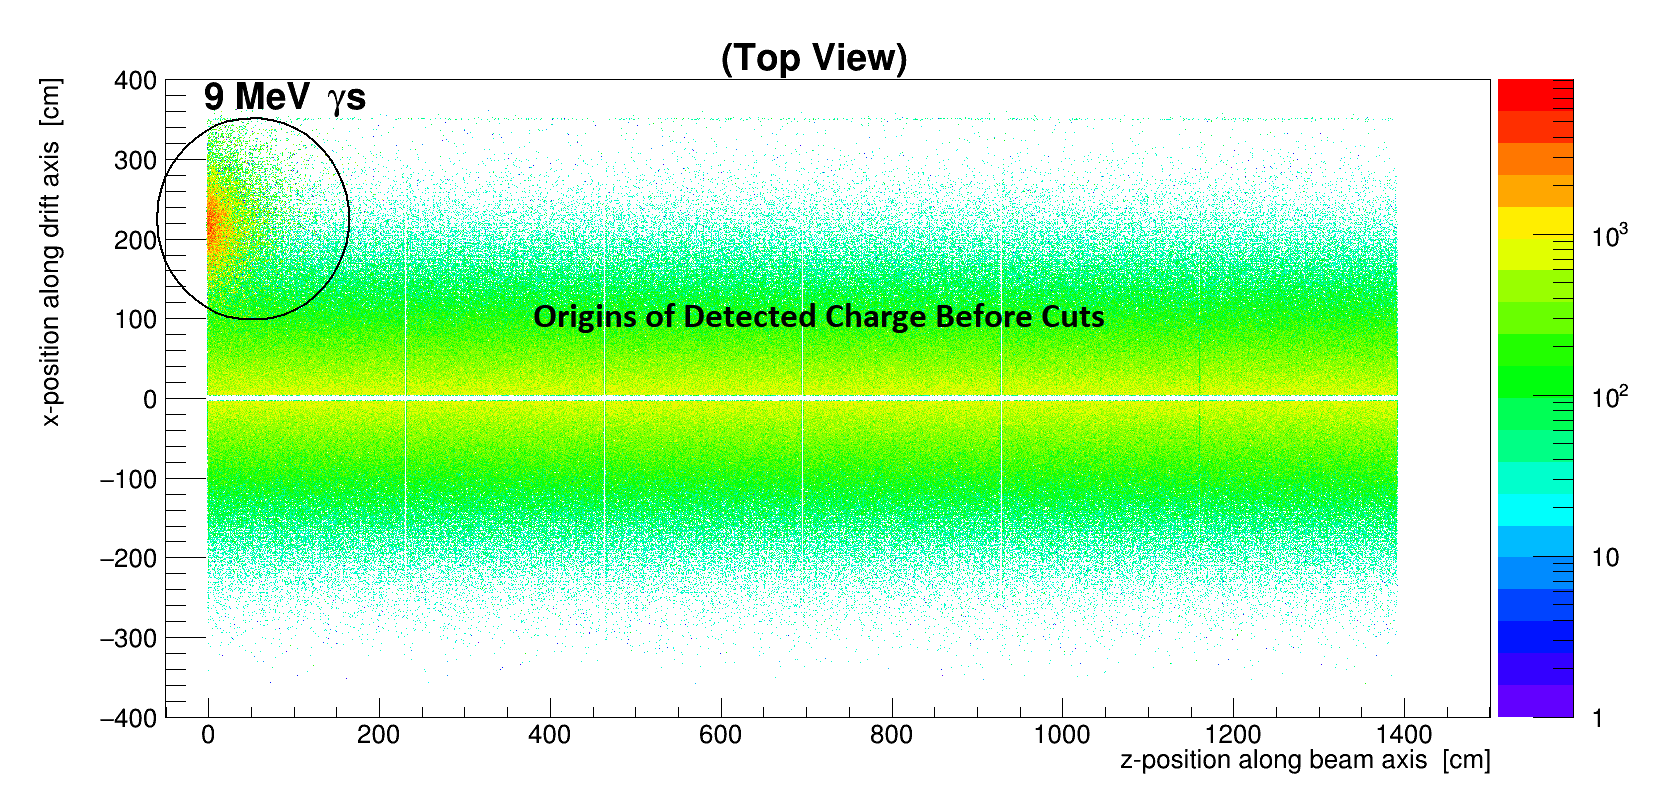
\includegraphics[width=1.0\linewidth]{9MeVgamma_withBG_LArSoft_v08_14_00_hiLY_originCHARGEcollected_TopView_TDR.png}
%   (b)
%   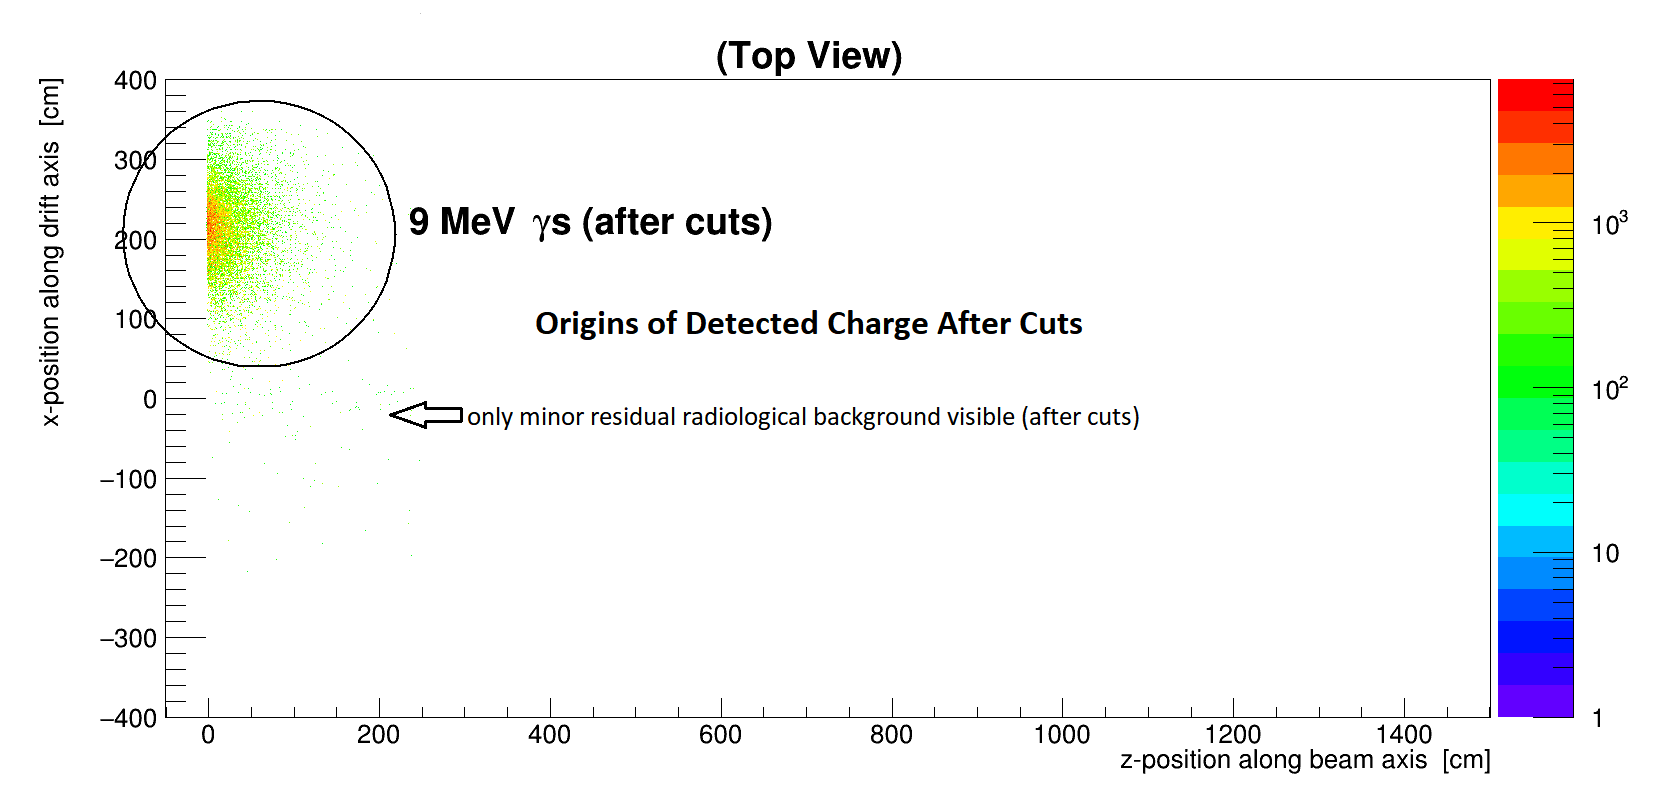
\includegraphics[width=1.0\linewidth]{9MeVgamma_withBG_LArSoft_v08_14_00_hiLY_originCHARGEcollected_TopView_cut_TDR.png}

%    \subfigure[a]{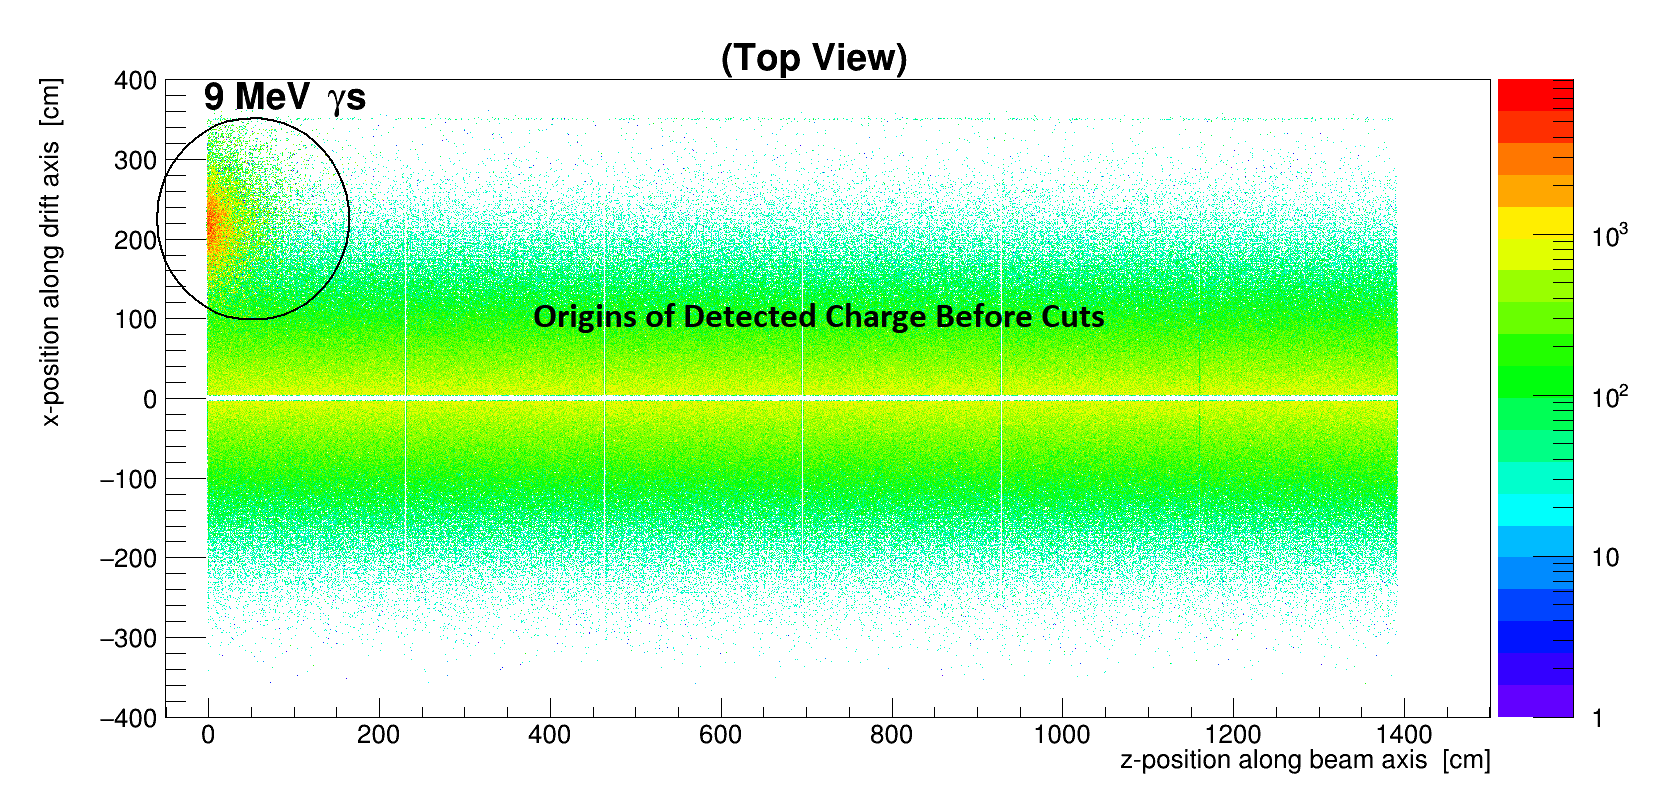
\includegraphics[width=1.0\linewidth]{9MeVgamma_withBG_LArSoft_v08_14_00_hiLY_originCHARGEcollected_TopView_TDR.png}}
%    \subfigure[b]{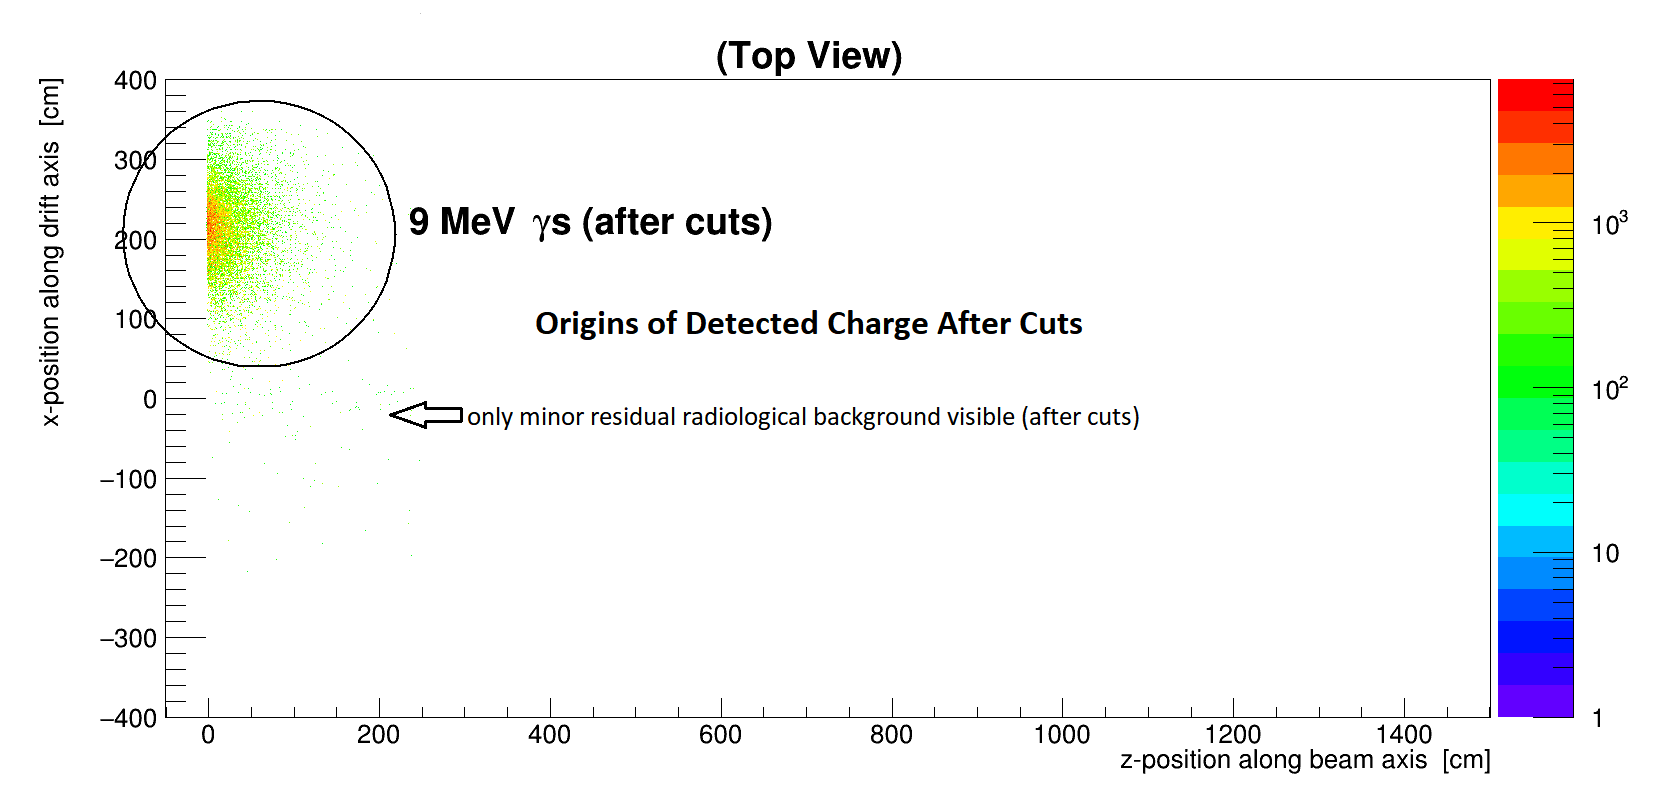
\includegraphics[width=1.0\linewidth]{9MeVgamma_withBG_LArSoft_v08_14_00_hiLY_originCHARGEcollected_TopView_cut_TDR.png}}
%\end{dunefigure}

%\begin{dunefigure}[Measurements of electric field strength and electron lifetime from 9 MeV gamma-ray source with radiological backgrounds]
%{fig:rsds-fig2}
%{fig:9MeVgamma_withBG_LArSoft_v08_14_00_hiLY_DriftTimesEfield_ChargeSpectrumElectronLifetime_cut}
%{Simulated measurements of (a) electric field strength from drift-time distribution, (b) electron lifetime from drift-time distribution, and (c) electron lifetime from charge distribution when electric field is unambiguously known from drift-time distribution. All spectra were created with applied selection cuts for a simulated 9~MeV $\gamma$-ray source with radiological backgrounds deployed at $z=$\SI{-40}{\cm} outside of the \dword{fc}, $x=$\SI{220}{\cm} away from the \dword{apa}, and $y=$\SI{300}{\cm} half-height of an upper endwall \dword{apa}. (Colors of histograms are matching colors of corresponding labels in each histogram.)}
%\centering
%    (a)
%    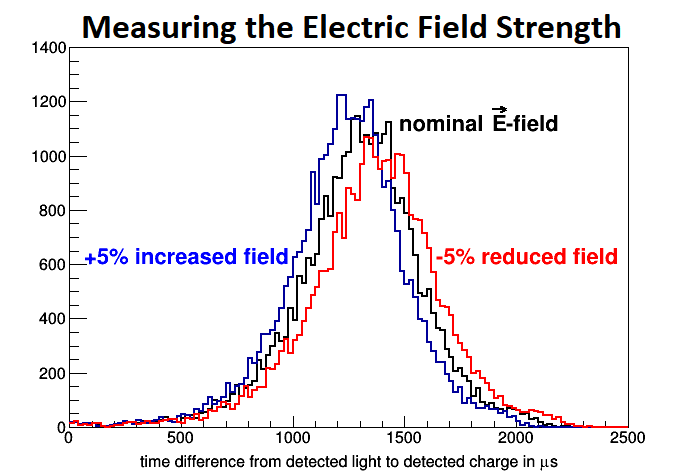
\includegraphics[width=0.45\linewidth]{9MeVgamma_withBG_LArSoft_v08_14_00_hiLY_EfieldDriftTimes_cut_TDR.png}
%    (b)
%    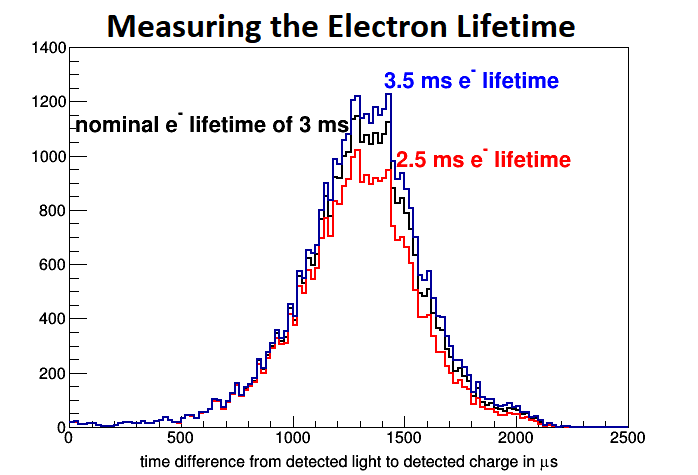
\includegraphics[width=0.45\linewidth]{9MeVgamma_withBG_LArSoft_v08_14_00_hiLY_eLifeTimeDriftTimes_cut_TDR.png}
%    (c)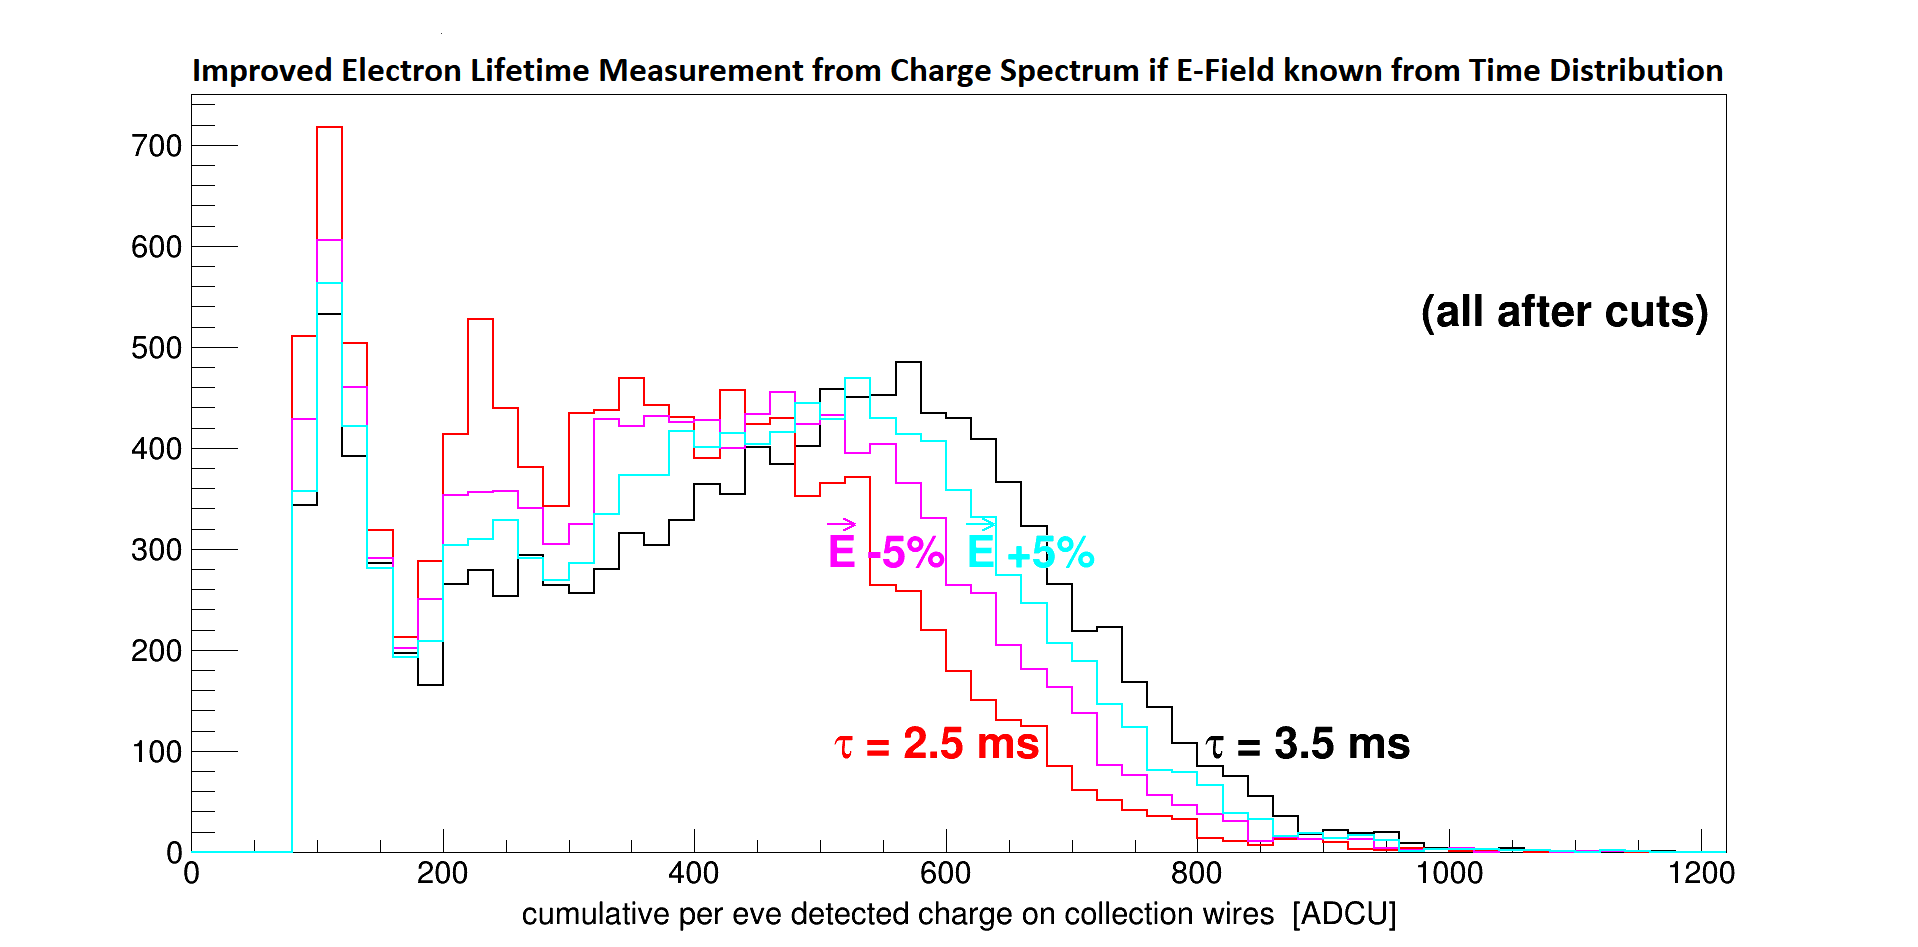
\includegraphics[width=1.0\linewidth]{9MeVgamma_withBG_LArSoft_v08_14_00_hiLY_chargeSpectrum_eLifeTimeEfield_cut_TDR.png}
    
%        \subfigure[a]{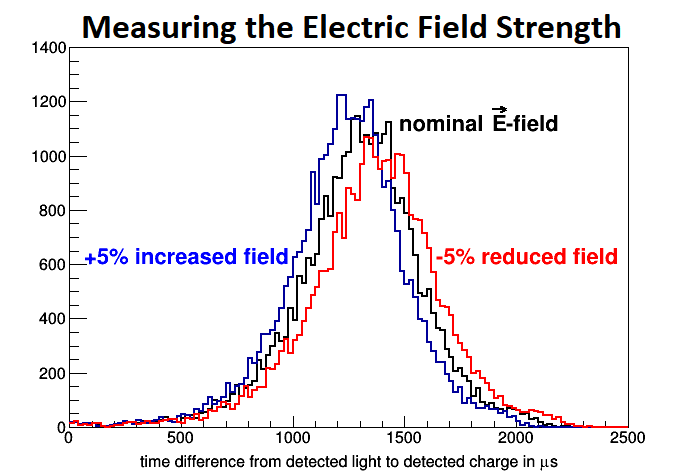
\includegraphics[width=0.45\linewidth]{9MeVgamma_withBG_LArSoft_v08_14_00_hiLY_EfieldDriftTimes_cut_TDR.png}}
%    \subfigure[b]{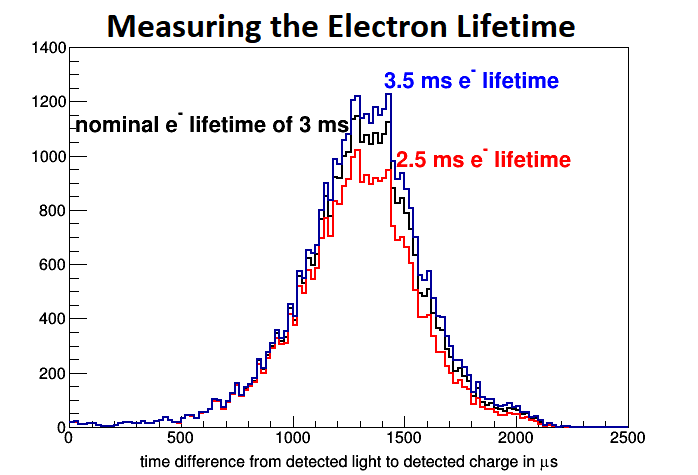
\includegraphics[width=0.45\linewidth]{9MeVgamma_withBG_LArSoft_v08_14_00_hiLY_eLifeTimeDriftTimes_cut_TDR.png}}
%    \subfigure[c]{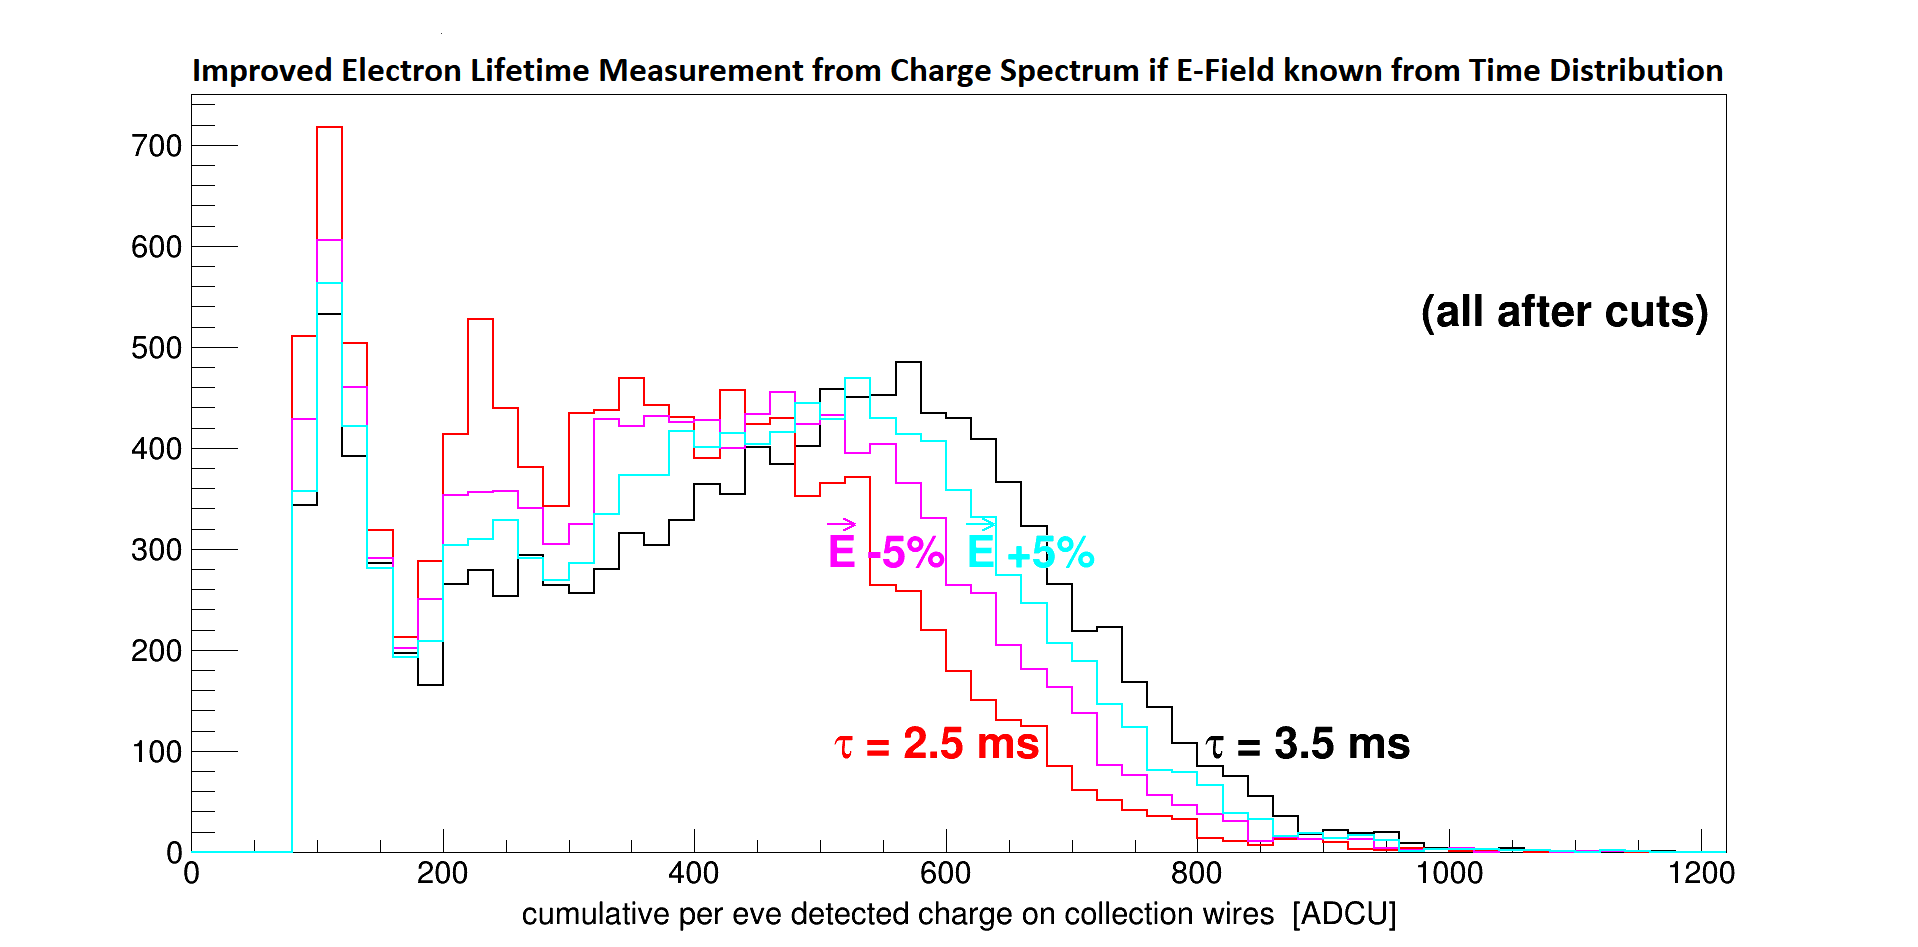
\includegraphics[width=1.0\linewidth]{9MeVgamma_withBG_LArSoft_v08_14_00_hiLY_chargeSpectrum_eLifeTimeEfield_cut_TDR.png}}
%\end{dunefigure}

%\begin{dunefigure}[Frequency of optical channel hits with a radioactive gamma-ray source with radiological backgrounds]
%{fig:rsds-fig2plus}
%{fig:5MeValphaSource_zx_TDR_TopView}
%{In LArSoft simulated change in frequency of optical channel hits with a simulated 9~MeV $\gamma$-ray source deployed at $z=$\SI{-40}{\cm} outside of the \dword{fc}, $x=$\SI{220}{\cm} away from the \dword{apa}, and $y=$\SI{300}{\cm} half-height of an upper endwall \dword{apa} with simulated expected radiological background.}
%  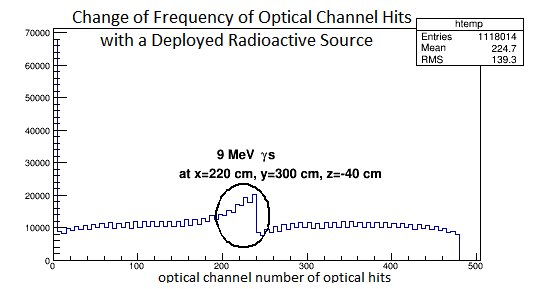
\includegraphics[width=0.6\linewidth]{ophit_opchannels_9MeVgammaSource_wBGs_LArSoft_v08_14_00_geo_v4_TDR.png}
%\end{dunefigure}


%\begin{dunefigure}[Detected light and charge from 15 MeV gamma-ray source without radiological backgrounds]
%{fig:rsds-fig3}
%{fig:5MeValphaSource_zx_TDR_TopView}
%{In LArSoft backtracked origins of detected (a) photoelectrons and (b) charge for a simulated $^{40}$Ar($\alpha,\,\gamma$)$^{44}$Ca 15~MeV $\gamma$-ray source deployed at $z=$\SI{-40}{\cm} outside of the \dword{fc}, $x=$\SI{220}{\cm} away from the \dword{apa}, and $y=$\SI{300}{\cm} half-height of an upper endwall \dword{apa} without simulated expected radiological background.}
%\centering
%   (a)
%   \includegraphics[width=0.455\linewidth]{5MeValphaSource_zx_pe_TDR.png}
%   (b)
%   \includegraphics[width=0.455\linewidth]{5MeValphaSource_zx_adc_TDR.png}
%\end{dunefigure}


\subsubsection{\dword{rsds} Design Validation}
%\dword{pddp} provides the ultimate test to validate the design, operation, and performance of the system and decide whether to deploy this system for the \dword{fd}. 
The cosmic induced background rate at \dword{protodune} is too high at the surface to detect responses to the \dword{dune} $\gamma$-ray source; however, the known deployment location along the vertical drift will allow a clear measurement of the electron lifetime and will help separate background events from calibration events, unlike in the \dword{pdsp} detector. Additionally, tests of functionality, reliability, and safety of the mechanical deployment system are needed to show the source can be deployed and retrieved with no issues.

%The source can be deployed to test the detector response and analysis method. 
%a higher intensity source could be deployed to test the detector response and analysis method. However, tests of functionality, reliability, and safety of the mechanical deployment system are needed to show the source can be deployed and retrieved with no issues. While these aspects can be largely tested in \dword{pdsp}-II, there are many \dual-specific aspects (e.g., 12~m long drift, sampling along the drift direction) that can benefit from a validation in \dword{pddp}-II.

Table~\ref{tab:calib-rsds-sched-dp} shows a schedule with the main steps for \dword{pddp}-II deployment.

\begin{dunetable}
[Key Milestones for Commissioning RSDS in ProtoDUNE-DP-II.] % Nonstandard for pdune 2
{p{0.65\textwidth}p{0.25\textwidth}}
{tab:calib-rsds-sched-dp}
{Key milestones towards commissioning the \dword{rsds} in \dword{pddp}-II.}  
Milestone & Date (Month YYYY)   \\ \toprowrule
Baseline \dword{rsds} design validation & January 2021 \\ \colhline 
\dword{rsds} mock-up deployment test at SDSMT & March 2021 \\ \colhline 
\dword{rsds} Design review  & May 2021 \\ \colhline
\dword{rsds} Production readiness review (PRR) & July 2021 \\ \colhline
Start of module 0 \dword{rsds} component production for ProtoDUNE-DP-II & September 2021      \\ \colhline
End of module 0 \dword{rsds} component production for ProtoDUNE-DP-II &  February 2022    \\ \colhline
\textbf{Start of ProtoDUNE-DP-II installation} & \textbf{March 2022} \\ \colhline
Start of \dword{rsds} installation &  April 2022    \\ \colhline
\dword{rsds} demonstration test at ProtoDUNE-DP-II  & April 2023\\ 
\end{dunetable}

\subsubsection{DAQ Requirements}
Section~\ref{sec:dp-calib-daqreq} provides an overall discussion of calibration and \dword{daq} interface. Here, the \dword{daq} requirements for the \dword{rsds} are discussed. The radioactive source will not be triggered by the \dword{mlt}, and the \isotope{Cf}{252} rate should be too high for a source tag to be useful.
%Rather, it will deliver a tag to the \dword{mlt} and that tag will include a time stamp that can be used by the \dword{mlt} to issue a trigger command to the \dword{fe} readout.  The trigger command will have a standard readout window size of \SI{16.4}{\milli\s}, but to keep data rates manageable, the command will only be send to \dword{fe} readout buffers that are expected to be illuminated by the source. The localization of trigger commands thus reduces the data volume by \num{150}, if only one %\dword{apa} 
%\dword{crp} is read out.

%\fixme{SG: In the previous sentence, I nominally changed APA to CRP but the data volume reduction for DP might need to be updated.}
%\fixme{SG: the next paragraph needs updating for DP. \\ 
%JM: Also because the source isn't tagged and the text assumes it is.}
If the rate of such a source is anywhere close to one per \SI{16.4}{\milli\s}, the detector would run continuously in the current scheme. Therefore, we assume that the interaction rate in the detector is \SI{10}{\hertz} or less. 

%The tag from the source will likely be much higher than this, because not all $\gamma$s interact in the active \dword{tpc} volume. Thus the radioactive source trigger will be a coincidence in the \dword{mlt} between a low-energy trigger candidate from the illuminated %\dword{apa}
%\dword{crp}, and a source tag with a relevant time stamp.  

With this rate, and with localization of events to one %\dword{apa}
\dword{crp} (\dpchpercrp channels), the total data volume would be
\begin{equation}
\num{8}~{\rm hours} \times \num{4}~{\rm FTs} \times \SI{10}{\hertz} \times \num{1.5}~{\rm Bytes}\times \SI{2}{\mega\hertz}\times \SI{16.4}{\milli\s}\times \num{1920}~{\rm channels} = \num{114}~{\rm TB/scan}.
\end{equation}
%SP
%\begin{equation}
%\num{8}~{\rm hours} \times \num{4}~{\rm FTs} \times \SI{10}{\hertz} \times \num{1.5}~{\rm Bytes}\times \SI{2}{\mega\hertz}\times \SI{5.4}{\milli\s}\times \num{2560}~{\rm channels} = \num{50}~{\rm TB/scan}.
%\end{equation}

%\fixme{Table 1.13 is not referenced in the text. It should be.}
%\fixme{OK. Please remove if OK.}
 Running this calibration twice per year would yield \num{228}~TB of data in \SI{10}{\kt} per year, see Table~\ref{tab:calib-daq-rsds}. By selecting only a fraction of the drift time range, it should be possible to reduce this estimate, or by increasing the calibration frequency, the total data volume can be kept. 
 
 \begin{dunetable}
[Calibration DAQ summary for RSDS]
{p{0.2\textwidth}p{0.15\textwidth}p{0.5\textwidth}}
{tab:calib-daq-rsds}
{Estimated uncompressed \dword{daq} data volume per year per \SI{10}{\kt} for the radioactive source system.}   
System & Data Volume (TB/year) & Assumptions  \\ \toprowrule
Proposed Radioactive Source System & \num{228} & Source rate < \SI{10}{\hertz}; single %\dword{apa} 
\dword{crp} readout,  lossless readout; \num{2} times/year   \\ 
\end{dunetable}   


\subsubsection{Risks}
The risks associated with the radioactive source system are described in Table~\ref{tab:risks:DP-FD-CAL-RSDS} along with appropriate mitigation strategies and the impact (low, medium or high risk levels) on probability, cost, and schedule post-mitigation. There are three residual medium-level risks in the table, more discussion on them is provided below:
\begin{itemize}
    \item {\it Radioactivity leak:} If radioactivity leaks into the detector during a deployment, radiological backgrounds in the detector might increase. Rigorous source certification under high pressure and cryogenic temperatures mitigates this risk.
    \item {\it Source stuck or lost:} If the source gets stuck or is lost in the detector, then it becomes a permanent localized radiological background source. Fish-line an order of magnitude stronger than needed to hold the weight, round edges of the moderator and a torque limit of the stepper motor will mitigate this risk.
    \item {\it Oxygen and nitrogen contamination:} If the purge-box has a small leak, oxygen and nitrogen could get into the \dword{lar}. Leak checks before deployments will mitigate this risk.
\end{itemize}


% risk table values for subsystem DP-FD-CAL-RSDS
\begin{footnotesize}
%\begin{longtable}{p{0.18\textwidth}p{0.20\textwidth}p{0.32\textwidth}p{0.02\textwidth}p{0.02\textwidth}p{0.02\textwidth}}
\begin{longtable}{P{0.18\textwidth}P{0.20\textwidth}P{0.32\textwidth}P{0.02\textwidth}P{0.02\textwidth}P{0.02\textwidth}} 
\caption[Risks for DP-FD-CAL-RSDS]{Risks for DP-FD-CAL-RSDS (P=probability, C=cost, S=schedule) More information at \dword{riskprob}. \fixmehl{ref \texttt{tab:risks:DP-FD-CAL-RSDS}}} \\
\rowcolor{dunesky}
ID & Risk & Mitigation & P & C & S  \\  \colhline
RT-DP-CAL-10 & Radioactive source swings into detector elements & Constrain the system with guide-wires & L & L & L \\  \colhline
RT-DP-CAL-11 & Radioactivity leak & Obtain rigorous source certification under high pressure and cryogenic temperatures & L & L & M \\  \colhline
RT-DP-CAL-12 & Source stuck or lost & Safe engineering margins, stronger fish-line and a torque limit in deployment system & L & M & L \\  \colhline
RT-DP-CAL-13 & Oxygen and nitrogen contamination & Leak checks before deployments & L & M & M \\  \colhline
RT-DP-CAL-14 & Light leak into the detector through purge-box & Light-tight purge box with an infrared camera for visual checks & L & L & L \\  \colhline
RT-DP-CAL-15 & Activation of the cryostat insulation & Activation studies and simulations & L & L & L \\  \colhline

\label{tab:risks:DP-FD-CAL-RSDS}
\end{longtable}
\end{footnotesize}

\begin{comment}
%SG: Old table of risks for RSDS.
\begin{dunetable}
[Calibration risks3]
{p{0.03\linewidth}p{0.4\linewidth}p{0.05\linewidth}p{0.4\linewidth}}
{tab:fdgen-calib-risks3}
{Possible risk scenarios for the radioactive source system along with mitigation strategies. The level of risk is indicated by letters ``H'', ``M'', and ``L'' corresponding to high, medium and low level risks.}   
No. & Risk  & Risk Level & Mitigation Strategy  \\ \toprowrule

10 & The deployed radioactive source can potentially swing into detector elements if not controlled or if large currents exist in the \dword{lar} & M & Guide-wires mitigate this risk.\\ \colhline

11 & Radioactivity could leak into the detector during a deployment. & L & Rigorous source certification under large pressure and cryogenic temperatures mitigates this risk.\\ \colhline

12 & The source could get stuck or lost in the detector. & L & Fish-line an order of magnitude stronger than needed to hold the weight, round edges of the moderator and a torque limit of the stepper motor will mitigate this risk.\\ \colhline

13 & Oxygen and nitrogen could get into the \dword{lar} in case the purge-box has a small leak. & M & Leak checks before deployments, purge-box in under-pressure inside w/r to the detector, will mitigate this risk.\\ \colhline

14 & Light could couple into the detector. & M &
Light-tight purge-box, internally equipped with an infra-red camera for visual checks will mitigate this risk.\\ \colhline

15 & The source activity can activate the cryostat insulation. & L & Detailed simulations/activation measurements can say what is a tolerable activity and the source activity can be chosen to be below that. \\ \colhline
\end{dunetable}
\end{comment}

\subsubsection{Installation, Integration, and Commissioning}
Before the \dword{tpc} elements are installed, the first elements of the radioactive source guide system are installed on the \endwall farthest from the \dword{tco}; it is the last system installed
%concurrent and coordinated with the alternative laser system (if any deployed), 
before the \dword{tpc} is installed and before closing the \dword{tco}. The radioactive source deployment system is installed at the top of the cryostat and can be installed when \dword{dune} becomes operational.

The commissioning plan for the source deployment system will include a dummy source deployment (within \num{2} of the commissioning) followed by first real source deployment (within \num{3} to \num{4} months of the commissioning) and a second real source deployment (within \num{6} of the commissioning). Assuming stable detector conditions, the radioactive source will be deployed every half a year. Ideally, a deployment before and after a run period are desired so at least two data points are available for calibration. This also provides a check if the state of the detector
has changed before and after the physics data run.
%If stability fluctuates for any reason (e.g., electronic response changes over time) at a particular location, one would want to deploy the source at that location once a month, or more often, depending on how bad the stability is.
It is estimated that it will take a few hours (e.g., \num{8}~hours) to deploy the system at one feedthrough location and a full radioactive source calibration campaign might take %at least 
a week.

%\newpage
\subsubsection{Quality Control}
A mechanical test of the Double Chooz fish-line deployment system with a \dword{lar} mock-up column will be done in the high bay laboratory at South Dakota School of Mines and Technology. The ultimate test of the system will be done at \dword{protodune}. Safety checks will also be done for the source and for appropriate storage on the surface and underground. 

\subsubsection{Safety}
\label{sec:dp-calib-rsds-safety}
A composite source is used for the radioactive source system that consists  of \isotope{Cf}{252}, a strong neutron emitter, and \isotope{Ni}{58}, which, via the \isotope{Ni}{58}(n,$\gamma$)\isotope{Ni}{59} process, converts one of the \isotope{Cf}{252} fission neutrons, suitably moderated, to a monoenergetic \SI{9}{\MeV} gamma. This system also poses a radiation risk, which will be mitigated with a purge-box for handling, and a shielded storage box and an area with lockout-tagout procedures, also applied to the gate-valve on top of the cryostat. Material safety data sheets will be submitted to \dword{dune} \dword{esh} and specific procedures will be developed for storage and handling of sources to meet Fermilab Radiological Control Manual (FRCM) requirements. These procedures will be reviewed and approved by \dword{surf} and \fnal radiation safety officers. Sources that get deployed will be checked monthly to ensure they are not leaking. A designated shielded storage area will be assigned for sources and proper handling procedures will be reviewed periodically. A custodian will be assigned to each shielded source.
%%%%%%%%%%%%%%%%%%%%%%%%%%%%%%%%%%%%%%%%%%%%%%%%%%%%%%%
%\section{Additional Systems Considered: External Muon Tracker}
%\label{sec:dp-calib-addl}
%%%%%%%%%%%%%%%%%%%%%%%%%%%%
%\subsection{External Muon Tagger}
%\fixme{you can't have just one subsection; if it's only the muon tagger, then let's put this in the section heading}
%\input{vol-dp/ch-dp-emt}

%%%%%%%%%%%%%%%%%%%%%%%%%%%%%%%%%%%%%%%%%%%%%%%%%%%%%%%
%\section{Cryostat Configuration for Calibration}
%\label{sec:dp-calib-cryocfg}

%%%%%%%%%%%%%%%%%%%%%%%%%%%%%%%%%%%%%%%%%%%%%%%%%%%%%%%  
%changed from subsection to section
\subsection{Validation of Calibration Systems}
\label{sec:dp-calib-val}
%%%%%%%%%%%%%%%%%%%%%%%%%%%%
%\subsection{Validation of Calibration Hardware Systems}

All calibration designs presented in the previous section require full system validation before being deployed in the \dword{dune} \dword{fd}. 

Although laser calibration systems are being operated in other \dword{lartpc} experiments (e.g., \dword{microboone}, future \dword{sbnd} runs), they have stringent requirements in terms of mechanical and optical precision , long-term reliability, laser track length, performance of the \dword{lbls}, \dword{daq} interface, and effect on \efield, especially due to the location of the periscope in the gap between the \dword{fc} and \dword{crp}. All of these lead to corresponding goals for a test installation and operation in \dword{pddp} that could be done in the post-LS2 run. 

We are currently considering available suitable ports in \dword{pddp} that can be used for these tests.
As Figure~\ref{fig:protoDUNEDP_topView_marked} shows, \dword{pddp} has ports the same size as the \dword{dune} \dword{fd} that could, in principle, be used for these tests.  If a pair of ports can be used, then one could even have crossing tracks within a single drift volume. However, the available ports are outside the \dword{tpc}, so coverage will be limited by shadowing from the \dword{fc}, and no reflector panels should be installed close to the laser periscopes.

\begin{dunefigure}[Top view of the \dword{pddp} cryostat showing various penetrations]{fig:protoDUNEDP_topView_marked}
{Top view of the \dword{pddp} cryostat showing various penetrations. Ports shown in red are marked as spares and, pending verification, could be used to test the calibration systems. These are the same diameter (\SI{250}{\milli\m} outer diameter) as the calibration ports of the \dword{dune} \dword{fd} and are located outside the \dword{tpc}. The largest port at the right side of the cryostat is a human access port.}
\includegraphics[height=4.0in]{protoDUNEDP_topView_marked.png}
\end{dunefigure}

The goal of validation would be to test all aspects of the system design, installation, alignment, operation, interfaces with \dword{daq}, and analysis, among others. \dword{pddp}, because it is located at the surface, could measure the \efield map with cosmics to compare with the one from the laser system to improve the analysis methods or identify weak points in the design. 
%An important design parameter is the length of a laser track. Our design assumes that \SI{12}{\m} is possible; \dword{microboone} has demonstrated only up to \SI{10}{\m}, but the track could be longer, depending on laser intensity. Measurements are limited by the size of the detector, but one way to gain information on longer tracks would be to make a scan with low laser intensities, so the end of the track would be visible and register how the maximum obtained track length scales with intensity. An extrapolation to the \dword{dune} \dword{fd} laser intensity would tell us the maximum length possible. Such a measurement could also be done at \dword{microboone}, \dword{sbnd}.

%\todo{SG: Jose, we had this paragraph on lifetime in SP, modify this for DP? it says APA in one sentence.}
An important aspect of the development plan, to be carried out at \dword{pddp}, is the characterization of the charge created by the laser beam ionization as a function of distance travelled in the \dword{lar} and the laser beam intensity. This dependence is thought to be affected by self-focusing effects due to the high light intensity, but it can be studied by measuring the collected charge distribution from a series of tracks close, and parallel, to the \dwords{crp} in order to break any correlations with the electron lifetime. This measured charge function could then be used with tracks in different directions to obtain a measurement of electron lifetime, which would significantly increase the capabilities of the laser system.  

The pulsed neutron source is a new idea never used in other experiments, so a \dword{pddp} test is essential. The corner human access ports similar to the ones in the \dword{dune} \dword{fd} could be used for this test.
%The post-beam run being proposed for ProtoDUNE-SP offers the opportunity to test the full system (DD Generator, Moderator, Transport Model, Data Analysis) in a definitive way before investing in the full PNS calibration for DUNE. The PNS group proposes to make such a run as soon as resources can be identified (independent of the other measurements above), starting with a commitment of engineering resources at CERN required to complete the necessary radiation safety shield design, and the mechanical design necessary to support the DD Generator and Moderator. The system used for ProtoDUNE-SP could also be used for ProtoDUNE-DP, and later installed in the DUNE detector. 

%For the radioactive source system, the cosmic induced background rate is too high at the surface to detect responses to the \dword{dune} gamma source; a higher intensity source could be deployed to test the detector response and analysis method. However, tests of functionality,  reliability, and safety of the mechanical deployment system are needed to show the source can be deployed and retrieved with no issues.

In addition to dedicated hardware validation runs at \dword{pddp}, other \dword{lar} experiments provide ample opportunities to develop and validate calibration tools and techniques, especially those relevant to the hardware being deployed. For example, the \dword{microboone} experiment is currently leading the development of analysis methods using laser data to extract an \efield map. Energy calibration techniques and related software tools are also being developed at various experiments (\dword{microboone}, ICARUS, \dword{lariat}, \dword{protodune}) that involve estimating and propagating uncertainties like \efield distortions, recombination, and other effects into physics signals. Other calibration related developments include \dword{daq} and calibration database design, all of which are being improved at \dword{sbn} and \dword{protodune}.
 
%%%%%%%%%%%%%%%%%%%%%%%%%%%%
%\subsubsection{Validation in Other Experiments}
%\label{sec:sp-calib-val-other}

%\cleardoublepage
%%%%%%%%%%%%%%%%%%%%%%%%%%%%%%%%%%%%%%%%%%%%%%%%%%%%%%%

\subsection{DAQ Requirements}
\label{sec:dp-calib-daqreq}
%\section{DAQ Requirements}
%\label{sec:sp-calib-daqreq}
%\fixme{JM/SG made edits. Josh K. to verify and sign off, especially the updated rates and assumptions there.}

The calibration systems must interface with the \dword{dune} \dword{daq} system, discussed in detail in Chapter~\ref{ch:dp-daq}. 
%%KMTDRREADME: This was directly repetitive with next paragraph
%Trigger decisions for physics events are done hierarchically: trigger primitives (TPs) are generated from\dword{crp} and \dword{pds} ``hits'', and these TPs are then used to create Trigger Candidates which are collections of TPs satisfying selection criteria such as exceeding a threshold number of adjacent \dword{crp} hits, or total  charge recorded, etc. These Trigger Candidates are passed on to a Module Level Trigger which then makes decisions about whether a given Trigger Candidate is accepted as a detector-wide trigger.  If so, the Module Level Trigger sends trigger commands to the Data Flow Orchestrator (DFO) which in turn passes them to an available Event Builder that then requests data from the Front-End Readout of the DAQ (servers that host FELIX cards). The management of trigger decisions---whether they are generated by candidates from the \dword{tpc}, \dword{pds}, calibrations, or other systems---is done in the \dword{mlt}.
%\fixme{add def to MLT in glossary}

Trigger decisions for physics events are made %done 
hierarchically: \dwords{trigprimitive} are generated from %\dword{tpc} 
\dword{crp} and \dword{pds} hits, and these \dwords{trigprimitive} are then used to create \dwords{trigcandidate}, which are collections of \dwords{trigprimitive} satisfying selection criteria such as exceeding a threshold number of adjacent 
%collection wire 
\dword{crp} hits, total 
%collection wire 
charge recorded, as well as other criteria. These \dwords{trigcandidate} are passed on to a \dword{mlt}, which then makes decisions about whether a given \dword{trigcandidate} is accepted as a detector-wide trigger.  If so, the \dword{mlt} sends trigger commands to the \dword{daqdfo}, which in turn passes them to an available \dword{eb} that then requests data from the \dword{fe} readout of the \dword{daq} (servers that host \dword{felix} cards). Managing \dwords{trigdecision}, whether they are generated by candidates from the \dword{tpc}, \dword{pds}, calibrations, or other systems, is done in the \dword{mlt}. 

The trigger commands are in the form of absolute time stamps that are used to extract snapshots of the data stored in the \dword{fe} readout buffers. For physics triggers, all \dword{tpc} information for a snapshot of time
%(roughly twice the drift time, or \SI{5.4}{\milli\s})
(\SI{16.4}{\milli\s}) %\todo{SG: readout time updated to 16.4 ms for DP. JK to sign off} 
are read out, without any additional zero suppression or localization. For calibration events, this approach would create an unmanageable amount of data and, in any case, is unnecessary because calibration events create interactions or tracks at known positions or times or both.

%The primary interface with calibrations will be through the DUNE timing system, which is responsible for synchronization across all subsystems and for providing absolute time stamps t. 

    
    To reduce data volume from calibrations, therefore, calibration systems that can be triggered externally are desirable. Like the distribution of trigger commands to the \dword{fe} readout buffers, the external trigger for a calibration system will take the form of an absolute time stamp. The time stamp is generated by the \dword{mlt}, thus ensuring that (for example) a calibration event does not occur during a candidate supernova burst.  These time stamps are distributed through the \dword{daq}'s timing and synchronization system. Thus, triggerable calibration systems (like the laser or \dword{pns}) must be synchronized to the rest of the \dword{daq} system and be capable of accepting time stamps.

There will be differences in the details of how different calibration systems are handled, as discussed below. \fixme{Tables (and figures) must be discussed in the text. This table is not discussed anywhere that I can see.}
           
\begin{dunetable}
[Calibration DAQ summary]
{p{0.2\textwidth}p{0.15\textwidth}p{0.5\textwidth}}
{tab:calib-daq}
{Estimated \dword{daq} rates per year per \SI{10}{\kt} for various calibration systems.}   
System & Uncompressed Data Volume (TB/year) & Assumptions  \\ \toprowrule
Ionization Laser System & \num{37} & \num{400}k laser pulses, \num{10}$\times$\num{10}$\times$\SI{10}{\cubic\cm} voxel sizes, a \SI{100}{\micro\s} zero suppression window (lossy readout), \num{2} times/year  \\ \colhline
Neutron Source System & \num{102} & \num{e6}~neutrons/pulse, \num{1000} neutron captures/m$^{3}$, \num{1300} observed neutron captures per pulse, \num{6}~times/year  \\ \colhline
%Proposed Radioactive Source System & \num{200} & Source rate < \SI{10}{\hertz}; single \dword{apa} readout,  lossless readout; \num{4} times/year   \\ \colhline
\end{dunetable}           
           
\subsubsection{Laser System}

%The proposed laser source is the only practical way to unambiguously measure the electric field vectors within the detector. 
The \efield vector from ionization laser calibration is determined by looking at the deflection of crossing laser tracks within detector voxels. The voxels are currently estimated at \num{10}$\times$\num{10}$\times$\SI{10}{\cubic\cm}. Because any given laser track
illuminates many such voxels, one laser pulse can be used for several
measurements; essentially, the number that matters is the area of each voxel.
The number of total laser events are estimated to be \num{400000}
%: about half the rate of cosmic rays 
and thus nominally produces a substantial total volume of data .

Fortunately, unlike every other event type in the detector, the laser track has both a reasonably well known position and time; thus the trigger command issued to the \dword{fe} buffers can be much narrower than the window used for physics triggers. A \SI{100}{\micro\s} zero suppression window should be wide enough to avoid windowing problems in the 
%induction plane wire \todo{SG:this sentence needs to be updated for DP}
signal deconvolution process. To ensure that the interesting part of each waveform is recorded, the \dword{daq} must know the current position  of the laser, which will be transmitted from the laser system to the \dword{mlt} via the \dword{daqccm}.

%\fixme{This estimate is dependent of assumptions that still need to be checked, namely that a zero suppression window \SI{100}{\micro\s} is still possible in DP, that the number of bytes per sample and the sampling rate are the same as in SP.} 

From the standpoint of data volume, therefore, the total, assuming the \SI{100}{\micro\s} zero-suppression window, is

%SP
%\begin{equation}
%\num{800000}/{\rm scan}/\SI{10}{\kt} \times \SI{100}{\micro\s} \times \num{1.5}{\rm Bytes/sample}\times \SI{2}{\mega\hertz}\times \num{384000}~{\rm channels}   = \num{92}~{\rm TB/scan/\SI{10}{\kt}.}   
%\end{equation}

%(\dpnumcrpch = 153 600 instead of \spnumch
% Scaling 92 * 400k/800k *153600/384k = 92*0.2 = 18.4
\begin{equation}
\num{400000}/{\rm scan}/\SI{10}{\kt} \times \SI{100}{\micro\s} \times \num{1.5}{\rm Bytes/sample}\times \SI{2}{\mega\hertz}\times \dpnumcrpch~{\rm channels}   = \num{18.4}~{\rm TB/scan/\SI{10}{\kt}.}   
\end{equation}


If such a calibration scan were done twice a year, then the total annual data volume for the laser is approximately \num{37}~TB/year/\SI{10}{\kt}.

\subsubsection{Pulsed Neutron Source}
%\todo{SG: JW to update this text and the number in the DAQ table 1.3.}
%There are two radioactive sources suggested to provide low-energy calibration data for DUNE: a neutron generator source, and a $\gamma$ source. 

The \dword{pns} system creates a burst of neutrons that
%, because of the interesting neutron cross section of argon, 
are captured throughout a large fraction of the total cryostat volume. For triggering and data volume, this is convenient: the existing scheme of taking \SI{16.4}{\milli\s} of data for each trigger means all these neutrons will be collected in a single \dword{dune} event.%\todo{SG: this requires updating since DP readout is not 5.4 ms} 
Thus, the data volume is simply \num{6.22}~GB times the total number of such pulses, but these are likely to be few: a single burst can produce thousands of neutrons whose $t_0$ is known up to the neutron capture time of \SI{200}{\micro\s} or so.

To trigger the \dword{pns}, the \dword{mlt} will provide a time stamp for the source to fire and then send a trigger command to the \dword{fe} readout buffers (via the \dword{daqdfo} and \dword{eb}) that will look like a physics trigger command.  The \dword{mlt} itself then tags that trigger command with the expected trigger type (in this case, \dword{pns}).

Typically, a commercial $DD$ neutron generator produces \num{e5} - \num{e8} neutrons/pulse, depending on the adjustable pulse width. The current assumption for neutron yield from the $DD$ generator is \num{e6} neutrons per pulse\footnote{Ideal assumption based on $DD$ generators that produce the highest neutron yield with a pulse width less than \SI{100}{\micro\s}. Such $DD$ generators are being developed in laboratories; commercial devices may require further development to reach this level of performance.}. With the current deployment designs in Figure~\ref{fig:PNS_Two_Designs}, approximately \num{1300} neutron captures per $DD$ generator pulse should be observed inside a \SI{10}{\kt} module. The suggested number for localized energy calibration is \num{1000} neutron captures per \si{\cubic\m}, so a total number of \num{4600} pulses would be needed to calibrate a \SI{10}{\kt} module. Assuming two identical \dwords{pns} operating in synchronization mode, \num{2300} pulses are needed for each calibration run. Therefore, the total data volume per run would be

%SP
%\begin{equation}
%\num{2300}~{\rm Pulses} \times \num{1.5}~{\rm Bytes}\times
%\SI{2}{\mega\hertz}\times \SI{5.4}{\milli\s}\times \num{384000}~{\rm channels} = %\num{14}~{\rm TB/run}.
%\end{equation}

%scale by 14 * 16.4/5.4 * 153600/384000 = 17
\begin{equation}
\num{2300}~{\rm Pulses} \times \num{1.5}~{\rm Bytes}\times
\SI{2}{\mega\hertz}\times \SI{16.4}{\milli\s}\times \dpnumcrpch~{\rm channels} = \num{17}~{\rm TB/run}.
\end{equation}

Running the \dword{pns} calibration system every two months would result in a total data volume of \num{102}~TB per \SI{10}{\kt} per year and running \num{12} times/year would result in \num{204}~TB/year per \SI{10}{\kt}. 

%\subsubsection{Proposed Radioactive Source System}

%The radioactive source will not be triggerable by the Module Level Trigger.  Rather, it will deliver a tag to the Module Level Trigger and that tag will include a time stamp that can be used by the Module Level Trigger to issue a trigger command to the Front-End Readout.  The trigger command will have a standard readout window size of \SI{5.4}{\milli\s}, but to keep data rates manageable, the command will only be send to Front-End Readout buffers that are expected to be illuminated by the source. The localization of trigger commands thus reduces the data volume by \num{150}, if only one \dword{apa} is read out.

 %Nevertheless, if the rate of such a source is anywhere close to one per \SI{5.4}{\milli\s}, the detector would be running  continuously in the current scheme. Therefore we assume that theinteraction rate in the detector is \SI{10}{\hertz} or less. The tag from the source will likely be much higher than this, because not all $\gamma$s interact in the active \dword{tpc} volume. Thus the radioactive source trigger will be a coincidence in the Module-Level Trigger between a low-energy trigger candidate from the illuminated \dword{apa}, and a source tag with a relevant time stamp.  With this rate, and with localization of events to one \dword{apa}, the total data volume would be

%\begin{equation}
%\num{8}~{\rm hours} \times \num{4}~{\rm FTs} \times %\SI{10}{\hertz} \times \num{1.5}~{\rm Bytes}\times %\SI{2}{\mega\hertz}\times \SI{5.4}{\milli\s}\times \num{2560}~{\rm %channels} = \num{50}~{\rm TB/scan}.
%\end{equation}

%Running this calibration four times/year would yield \num{200}~TB of data in \SI{10}{\kt} per year.


\begin{comment}
%SG: This is not under the scope of this chapter. Needs to be moved to physics. 
\fixme{I did go ahead and edit this, but apparently it goes elsewhere in the manuscript.}
\subsubsection{Intrinsic Radioactivity}

Mike Mooney has suggested using the intrinsic \Ar39 as a calibration source. This has many advantages over either of the radioactive
source calibrations, in particular the known level of \Ar39, its uniform distribution in the detector, and the fact that it is always there and therefore integrates correctly over the detector lifetime. The difficulty is
that, because any individual \Ar39 event's $x$ position is not known
because there is no $t_0$, the distribution of these events must be used to
make measurements, thus requiring fairly high statistics.

Mooney's proposal is that roughly \num{250000} \Ar39 can provide a \SI{1}{\%} measurement of electron lifetime. (Note that \SI{1}{\%} is a reasonable goal;
if the lifetime and maximum drift time are the same, this results in a \SI{2}{\%} uncertainty on energy scale, which would begin to compromise \dword{dune}'s physics program). This number of events is easily obtained with the existing random triggers as well as every other trigger source excluding laser pulses and front-end calibrations.

Like all other parameters that must be calibrated, however, what is not
clear is what the spatial and temporal variations will be in the detector.
Other \dword{lar} \dword{tpc}s have performed lifetime calibrations daily (using cosmic rays
primarily), and a pixelization of \SI{1}{\square\m} is not unreasonable, leading to a
need for \num{250000} events for every \si{\square\m} in the detector each day, or about a \SI{1}{\hertz} trigger rate.

In the existing scheme, this would be overwhelmingly the dominant source of data. Thus either the pixelization must be reduced (say, to each of the \dword{tpc} volumes) or a zero-suppression scheme must be used.
Such a zero-suppression scheme would happen post-trigger (for example, running
random triggers at \SI{1}{\hertz} and based upon that trigger type, zero suppressing
signals). In the current scheme, this would happen in the event builder, but at \SI{1}{\hertz}, the data rate would be too high. To do zero suppression upstream (perhaps in the \dword{apa}-level readout) based on the trigger type will likely require more
hardware resources.
\end{comment}

%\subsection{External Muon Tracker}

%        An External Muon Tracker (EMT) has also been proposed, likely as a scintillator-bar telescope at the front face of the detector. The EMT would be intended to trigger on rock muons and provide a known entry position and direction for these. It is thus the only way to test reconstruction in the DUNE FD for a sample of events in the same energy regime as the beam events.

%        Because the EMT is measuring events that will already be triggered by the \dword{tpc}, the additional data volume comes only from the scintillator counters themselves. Because the only information needed for these events is the time of a hit in each counter, and because only four counters are likely to be hit by each muon (two planes of $x$ and $y$), the additional data rate from the EMT is very small.  If we limit ourselves to just the rock muons and assume that four counters are hit resulting in 4 12-bit words/counter (one charge and one time each, plus the counter ID and a local timestamp, then we get a yearly total data volume of
%\begin{equation}
%735{\rm year/10 ktonne} \times 24~{\rm B/event} = 17.6~{\rm kB/year}   
%\end{equation}
%%%%%%%%%%%%%%%%%%%%%%%%%%%%%%%%%%%%%%%%%%%%%%%%%%%%%%%  
\section{Organization and Management}
\label{sec:dp-calib-org}
%\fixme{SG/JM done! Needs updated chart from David replacing CE to CRP.}
The calibration consortium was formed in November 2018 as a joint single and dual phase consortium, with a consortium leader and a technical leader. Figure~\ref{fig:orgchart} shows the organization of the consortium. The calibration consortium board currently comprises institutional representatives from 11 institutions as shown in Table~\ref{tab:gen-calib-org}. The consortium leader is the spokesperson for the consortium and responsible for the overall scientific program and managing the group. The technical leader of the consortium manages the project for the group. 

The consortium's initial mandate is the design and prototyping of a laser calibration system, a neutron generator, and possibly a radioactive source system, so the consortium is organized into three working groups, each dedicated to one system. Each group has a designated working group leader.
The \dword{tdr} editors are responsible for the overall editing and delivery of the \dword{tdr} document.


\begin{dunefigure}[Organizational chart for the calibration consortium]{fig:orgchart}
{Organization chart for the calibration consortium.}
\includegraphics[height=3.0in]{orgchart-dp.png}
\end{dunefigure}


\begin{dunetable}
[Calibration Consortium Institutions]
{p{0.7\textwidth}c}
{tab:gen-calib-org}
{Current calibration consortium board institutional members and countries.}
Member Institute     &  Country       \\
Laboratorio de Instrumentacao e Fisica Experimental de Particulas (LIP) & Portugal \\ \colhline
University of Bern (Bern) & Switzerland \\ \colhline
Boston University (BU) & USA \\ \colhline
University of California, Davis (UC Davis)& USA \\ \colhline
Colorado State University (CSU) & USA \\ \colhline
University of Hawaii (Hawaii) & USA \\ \colhline
University of Iowa & USA \\ \colhline
Michigan State University (MSU) & USA \\ \colhline
University of Pittsburgh (Pitt) & USA \\ \colhline
South Dakota School of Mines and Technology (SDSMT) & USA \\ \colhline
University of Tennessee, Knoxville (UTK) & USA \\ 
\end{dunetable}

In addition, Figure~\ref{fig:orgchart} shows several liaison roles 
%\todo{These are being established after we have had initial interfaces and critical issues clarified} 
to facilitate connections with other groups and activities:
\begin{itemize}
    \item Detector integration and installation,
    \item Electrical and safety issues,
    \item \dword{daq},
    \item Computing,
    \item Cryogenic instrumentation and slow controls (CISC),
    %\item Cold electronics,
    \item \dword{crp},
    \item \dword{hv},
    \item Photon detection system.
\end{itemize}

%\fixme{KM adjusted above from "planned" to state will exist by Summer 2019}

Currently, new institutions are added to the consortium following an expression of interest from the institute and upon obtaining consensus from the current consortium board members.

%if the consortium board members agree, new members are added from other institutions if the new institutions express an interest through a petition to the board.
%%%%%%%%%%%%%%%%%%%%%%%%%%%%%%%%%%%%%%%%%%%%%%%%%%%%%%%
\subsection{Institutional Responsibilities}
\label{sec:dp-calib-resp}

%%%%%%%%%%%%%%%%%%%%%%%%%%%%%%%%%%%%%%%%%%%%%%%%%%%%%%%
%\section{Institutional Responsibilities}
%\label{sec:sp-calib-resp}

%\fixme{SG/JM: Done. KM: take a look. More details in the email I sent. }
%Currently, the calibration consortium has the following member institutions: University of Bern (Bern), Boston University (BU), Colorado State University (CSU), University of California, Davis (UC Davis) University of Hawaii (Hawaii), University of Iowa (Iowa), LIP, Michigan State University (MSU), University of Pittsburgh (Pitt), South Dakota School of Mine Technology (SDSMT), and University of Tennessee, Knoxville (UTK). 
%\fixme{SG:reviewed this and all looks good for DP! JM: reviewed, signing off}
Calibrations will be a joint effort for \dword{sp} and \dword{dp}. Design validation, testing, calibration, and performance of calibration devices will be evaluated using \dword{protodune} data.

Following the conceptual funding model for the consortium, various responsibilities have been distributed across institutions within the consortium. At this stage of the project, these are still aspirational responsibilities until firm funding is established. Table~\ref{tab:calib-inst-resp} shows the current institutional responsibilities for primary calibration subsystems. 
%Only lead institutes are listed in the table for a given effort. 
A number of institutions are interested in physics and simulations studies and validation with \dword{protodune}. A 
\dword{dune} DocDB will be prepared to provide a detailed list of tasks and corresponding institutional responsibilities.

%The responsibilities of each group are described in Table~\ref{tab:calibinst}. \fixme{Need to confirm this with groups, esp CSU, Pitt doing general simulation work and understand what further subdivision is useful. We are also seeking new groups.}

\begin{comment}
\begin{dunetable}
[Institutional responsibility for calibrations]
{p{0.25\textwidth}p{0.65\textwidth}}
{tab:calib-inst-resp}
{Institutional responsibilities in the calibration consortium.}   
System & Institutional Responsibility \\ \toprowrule
Laser System & Bern, Hawaii, LIP, Pitt, UTK \\ \colhline
Pulsed Neutron Source & BU, CSU, UC Davis, Iowa, LIP, MSU, SDSMT \\ \colhline
\end{dunetable}
\end{comment}

\begin{dunetable}
[Institutional responsibility for calibrations]
{p{0.25\textwidth}p{0.65\textwidth}}
{tab:calib-inst-resp}
{Institutional responsibilities in the Calibration Consortium}  Subsystem & Institutional Responsibility \\ \toprowrule
Ionization Laser System & Bern, LIP, UTK, Hawaii \\ \colhline 
Laser Positioning System & Hawaii, LIP \\ \colhline 
Photoelectron Laser System & UTK, Hawaii \\ \colhline
Pulsed Neutron Source System & BU, CSU, UC Davis, Iowa, LIP, MSU, UTK, SDSMT \\ \colhline
Proposed Radioactive Source System & SDSMT \\ \colhline
Physics \& Simulation & BU, CSU, Hawaii, UTK, LIP, MSU, SDSMT, UC Davis, Pittsburgh, Iowa \\ \colhline 
\end{dunetable}
%%%%%%%%%%%%%%%%%%%%%%%%%%%%%%%%%%%%%%%%%%%%%%%%%%%%%%%
\subsection{Cost and Labor}
\label{sec:dp-calib-cost}

%\fixme{KM/JM: Done; SG check?}
%KM: I am OK with this, let's see what the editors hate. \fixme{SG: done checking; 1. photoelectron laser missing from the table. Added it. 2. Updated the text to clearly state what the cost estimates include; 3. added some description for labor and a table with placeholders for actual labor hours. 4. The way it is currently split in the cost table, using the same rows will be tricky for labor hours. E.g. for the laser itself, no significant labor is associated. So, for the labor table, although it inconsistent with the cost table, I listed each of our devices as one entity. check if you are okay with this. Alternatively, we can lump everything into one system for the cost table as well so both tables are consistent which is what is expected from main editors. 5. I added a new category for labor, "physics & simulation" as those hours will also need to accounted for. }
%\fixme{SG/JM done; PE laser quantity to be reviewed, emailed Jelena;}

\fixme{cost and labor hour tables will be automated, template to come! Anne}

\begin{dunetable}
[Calibration System Cost Summary]
{p{0.15\textwidth}p{0.1\textwidth}p{0.15\textwidth}p{0.4\textwidth}}
{tab:calib-cost}
{Cost estimates for different calibration subsystems.}   
System & Quantity & Cost (under development) (k\$ US) & Description \\ \toprowrule
laser & 12 & - & high intensity laser source for laser system  \\ \colhline
laser optics module & 12 & -&  insulator ingress into detector and flange interface, mirrors, power, cables for laser system, and positioning system \\ \colhline
Photoelectron system & 4000 & - & includes targets to be mounted, both dots and strips, along with optical fibers to illuminate the photoelectric targets on two cathode planes, on both sides of each  cathode plane \\ \colhline 
DD generator device for \dword{pns}  & 2 &- & neutron source for \dword{pns} system \\ \colhline
Other \dword{pns} components  & 2 & - & includes moderator, surrounding shielding and neutron monitor \\ \colhline
%laser device & 17 & \num{50.0} & Laser system \\ \colhline
%feedthrough interface & 20 & \num{100.0} & Laser system; includes insulator ingress into detector and flange interface, mirrors \\ \colhline
%DD generator device  & 2 & \num{102.5} & \dword{pns} \\ \colhline
%Moderator  & 2 & \num{25.1} & \dword{pns}: materials to degrade neutrons to correct energy \\ \colhline
%Shielding & 2 & \num{24.0} & \dword{pns}: surrounding shielding \\ \colhline
% Monitor  & 2& \num{16.7} & \dword{pns}: Neutron monitor (device) and colimator (materials)  \\ \colhline
\end{dunetable}

\begin{dunetable}
[Calibration labor]
{p{0.25\textwidth}p{0.15\textwidth}p{0.1\textwidth}p{0.08\textwidth}p{0.08\textwidth}p{0.1\textwidth}p{0.08\textwidth}}
{tab:calib-labor}
{Labor hour estimates.}
System  & Faculty/Scientist & Post-doc & Student & Engineer & Technician  &  \textbf{Total}\\ \toprowrule
& (hours) & (hours)& (hours)& (hours)& (hours)& (hours)\\ \toprowrule
Ionization Laser system & -& -& -& -& - & - \\ \colhline
Photoelectron Laser system & -& -& -& -& - & - \\ \colhline
Laser positioning system & -& -& -& -& - & - \\ \colhline
\dlong{pns} system & -& -& -& -& - & - \\ \colhline
Physics \& Simulation & -& -& -& -& - & - \\ \colhline
\end{dunetable}

%\todo{SG: need quantity for photoelectron laser in the table 1.6.} KM: Quantity added from Jelena.
Table \ref{tab:calib-cost} shows the current cost estimates for the calibration subsystems. It also shows the quantity associated with each subsystem and a brief description of what is included in the cost estimate. The cost estimates include only materials and supplies (M\&S) \fixme{M\&S, as an abbreviation, is not in the glossary and is used only here. It should be eliminated.}and packing and shipping, but not labor and travel costs. One \dword{dp} detector module requires \num{12} ports for the laser (see Figure~\ref{fig:DPFDLaserPositions}), and each port needs one laser and one feedthrough interface. 
%; \num{14} ports will each need one laser and one feedthrough interface, but for the \num{6} ports central to the cryostat, one laser will service two ports. 
According to simulation studies, one \dword{dp} module requires two pulsed neutron systems.

Labor costs depend on personnel category (e.g., faculty, student, technician, post-doc, engineer) and vary by region and institution, so costs are quantified using labor hours needed to complete a given task. Table~\ref{tab:calib-labor} provides estimates of labor hours for each subsystem. 
%, for a total of \num{95010} labor hours for all calibration tasks. 



%The costs of equipment and materials and supplies for the baseline systems are described in Table~\ref{tab:calibcostsumm}. To serve one SP detector module, there are 20 ports for the laser (see figure~\ref{fig:ftmap}); 14 ports will each need one laser and one feedthrough interface, but for the 6 ports central to the cryostat, one laser will service two ports. Two pulsed neutron systems are needed for one SP module. % The total cost of the baseline calibration systems therefore is \$3.4M.
%\fixme{Add estimate of laser positioning system, DAQ/computers, racks? cables?}
%\fixme{Jose to get a cost from Jelena for position system, and photoelectron }
%%%%%%%%%%%%%%%%%%%%%%%%%%%%%%%%%%%%%%%%%%%%%%%%%%%%%%%
\subsection{Schedule and Milestones}
\label{sec:dp-calib-sched}
%\section{Schedule and Milestones}
%\label{sec:sp-calib-sched}

%\fixme{JM: Done; SG/KM: take a look}

%From Anne: This is a standard table template for the TDR schedules.  It contains overall FD dates from Eric James as of March 2019 (orange) that are held in macros in the common/defs.tex file so that the TDR team can change them if needed. Please do not edit these lines! Please add your milestone dates to fit in with the overall FD schedule. 
%\fixme{please use this schedule/milestones format}
%\fixme{SG: schedule table and text updated for DP; JM signed off}
%\fixme{The table does not appear in the PDF.SG:I checked it appears in the PDF now.}
\begin{dunetable}
[Key calibration construction milestones for commissioning of the first \dshort{dpmod}.]
{p{0.65\textwidth}p{0.25\textwidth}}
{tab:calib-sched-dp}
{Key calibration construction schedule milestones leading to the commissioning of the first \dword{dpmod}. (*) Schedule items related to the \dlong{rsds} (\dshort{rsds}) are to be considered pending system approval.}   
Milestone & Date (Month YYYY)   \\ \toprowrule
%Technology Decision Dates &      \\ \colhline
%Final Design Review Dates &      \\ \colhline
Laser systems design decision (including ionization, beam location and photoelectron systems) & January 2021 \\ \colhline 
Laser systems design review & February 2021 \\ \colhline 
%Ionization  laser design decision & August 2019 \\ \colhline
%Laser positioning system design decision & September 2019 \\ \colhline
%Photoelectron laser design decision & October 2019 \\ \colhline
\dword{pns} design decision  & March 2021 \\ \colhline
Start of module 0 component production for ProtoDUNE-II & March 2021      \\ \colhline
\rowcolor{dunepeach} Start of \dword{pdsp}-II installation& \startpduneiispinstall      \\ \colhline
\dword{pns} design review & April 2021 \\ \colhline
\dword{rsds} design review & May 2021 \\ \colhline
End of module 0 component production for ProtoDUNE-II &  January 2022    \\ \colhline

\rowcolor{dunepeach} Start of \dword{pddp}-II installation& \startpduneiidpinstall      \\ \colhline
 %\dword{prr} dates &      \\ \colhline
 %\dword{prr} dates &   March 2022   \\ \colhline
%Start of  (component 1) production  &      \\ \colhline
%Start of (component 2) production  &      \\ \colhline
%Start of  (component 3) production  &      \\ \colhline
\rowcolor{dunepeach}South Dakota Logistics Warehouse available& \sdlwavailable      \\ \colhline
\rowcolor{dunepeach}Beneficial occupancy of cavern 1 and \dword{cuc}& \cucbenocc      \\ \colhline
\dword{prr} dates &   March 2023   \\ \colhline
\rowcolor{dunepeach} \dword{cuc} counting room accessible& \accesscuccountrm      \\ \colhline
\dword{rsds} demonstration test at ProtoDUNE-DP-II (*) &   April 2023   \\ \colhline
Start of  Laser, \dword{pns} and \dword{rsds} (*) production  &   May 2023   \\ \colhline
\rowcolor{dunepeach}Top of \dword{detmodule} \#1 cryostat accessible& \accesstopfirstcryo      \\ \colhline
End of \dword{pns} production & March 2024 \\ \colhline 
Start assembly of calibration production units in the cavern & May 2024\\ \colhline
End of Laser system production  & July 2024     \\ \colhline
End of \dword{rsds} production (*) & August 2024     \\ \colhline
%Start installation and alignment of Laser boxes & May 2024 \\ \colhline 
%End of  (component 1) production  &      \\ \colhline
%... & ...                       \\ \colhline
\rowcolor{dunepeach}Start of \dword{detmodule} \#1 TPC installation& \startfirsttpcinstall      \\ \colhline
%Start installation of Laser System periscopes & August 2024 \\ \colhline 
%Start installation of \dword{rsds} guide system (*) & August 2024 \\ \colhline 
\rowcolor{dunepeach}Top of \dword{detmodule} \#2 accessible& \accesstopsecondcryo      \\ \colhline
\rowcolor{dunepeach}End of \dword{detmodule} \#1 TPC installation& \firsttpcinstallend      \\ \colhline
%Installation of \dword{rsds} purge-boxes (*) & May 2025 \\ \colhline 
%Installation of the \dword{pns} main components & June 2025 \\ \colhline

Start installation and alignment of Laser boxes & May 2025 \\ \colhline 
 \rowcolor{dunepeach}Start of \dword{detmodule} \#2 TPC installation& \startsecondtpcinstall      \\ \colhline
Start installation of Laser System periscopes & August 2025 \\ \colhline 
Start installation of \dword{rsds} guide system (*) & August 2025 \\ \colhline 
\rowcolor{dunepeach}End of \dword{detmodule} \#2 TPC installation& \secondtpcinstallend      \\ 
Installation of \dword{rsds} purge-boxes (*) & May 2026 \\ \colhline 
Installation of the \dword{pns} main components & June 2026 \\ 
%last item & ...                         \\
\end{dunetable}

Table~\ref{tab:calib-sched-dp} shows the schedule and key milestones for the calibration consortium that lead to commissioning the second \dword{fd} module. The demonstration of the calibration systems design, operation, and performance at the \dword{pddp}-II running is a key part of calibration schedule; those milestones are also listed in the table. The technology design decisions on calibration subsystems should be made by January 2021 for the laser system and by March 2022 for the neutron source system followed by technical design reviews. The production of the design prototypes to be deployed at \dword{pddp}-II running should be finished by January 2022 followed by assembly and deployment in \dword{pddp} in March 2022. The \dword{rsds}
%radioactive source deployment system (RSDS) \fixme{This abbreviation is in neither the common glossary nor the manuscript glossary. Is it necessary to abbreviate this at all? SG: yes, can Anne/Nora take care of this?}
design will follow a demonstration R\&D program outlined in detail in Table~\ref{tab:calib-rsds-sched-dp} in the appendix, with major milestones highlighted in this section. The major steps for systems approval are the design review in May 2021 and the deployment test at \dword{pddp}-II in April 2023. 

Production of calibration systems for the \dword{fd} should start in March 2023, followed by assembly of the systems underground once the detector cavern becomes available in early 2024. Installing the laser system can begin as soon as the cryostat roof is accessible and conclude once the \dword{tpc} is ready to install. If it is approved, the \dword{rsds} guide system can begin installation just before \dword{tpc} is installed. The purge-boxes on top of the cryostat can be done later.
Installing the main components of the \dword{pns} will begin once the human access ports are no longer needed for \dword{tpc} installation in June 2026. 

%Table~\ref{tab:pnssched} shows the milestones for the Pulsed Neutron System. \fixme{The laser system schedule will look similar to the pulsed neutron source-- but we need to confirm the TCO closing/installation period before filling in a table for it.}

\begin{comment}
%SG: old table
\begin{dunetable}
[Key calibration construction milestones for commissioning of the first \dword{spmod}.]
{p{0.65\textwidth}p{0.25\textwidth}}
{tab:calib-sched}
{Key calibration construction schedule milestones leading to commissioning the first \dword{fd} module. (*) Schedule items related to the \dword{rsds} are to be considered pending system approval.}  
Milestone & Date (Month YYYY)   \\ \toprowrule
%Technology Decision Dates &      \\ \colhline
Laser systems design decision (including ionization laser, laser positioning and photoelectron laser) & January 2020 \\ \colhline 
Laser systems design review & February 2020 \\ \colhline 
%Ionization  laser design decision & August 2019 \\ \colhline
%Laser positioning system design decision & September 2019 \\ \colhline
%Photoelectron laser design decision & October 2019 \\ \colhline
\dword{pns} design decision  & March 2020 \\ \colhline
\dword{pns} design review & April 2020 \\ \colhline
\dword{rsds} design review & May 2020 \\ \colhline
%Final Design Review Dates &      \\ \colhline
Start of module 0 component production for ProtoDUNE-II & April 2020      \\ \colhline
End of module 0 component production for ProtoDUNE-II &  February 2021    \\ \colhline
\textbf{Start of ProtoDUNE-SP-II installation} & \textbf{March 2021} \\ \colhline
%\textbf{Start of ProtoDUNE-DP-II installation} & \textbf{March 2022} \\ \colhline
%\rowcolor{dunepeach} Start of \dword{pdsp}-II installation& \startpduneiispinstall      \\ \colhline
%\rowcolor{dunepeach} Start of \dword{pddp}-II installation& \startpduneiidpinstall      \\ \colhline
 \dword{prr} dates &   March 2022   \\ \colhline
%Start of \dword{pns} production  &   May 2022   \\ \colhline
%Start of  (component 3) production  &      \\ \colhline
\textbf{South Dakota Logistics Warehouse available} & \textbf{\sdlwavailable}      \\ \colhline
\dword{rsds} demonstration test at ProtoDUNE-SP-II (*) &   April 2022   \\ \colhline
Start of  Laser and \dword{pns} production  &   May 2022   \\ \colhline
\textbf{Beneficial occupancy of cavern 1 and \dword{cuc}} & \textbf{\cucbenocc}      \\ \colhline
End of \dword{pns} production & March 2023 \\ \colhline 
End of Laser system production  & July 2023     \\ \colhline
End of \dword{rsds} production (*) & August 2023     \\ \colhline
%... & ...                       \\ \colhline
\textbf{\dword{cuc} counting room accessible} &  \textbf{\accesscuccountrm}      \\ \colhline
Start assembly of calibration production units in the cavern & May 2023\\ \colhline
\textbf{Top of \dword{detmodule} \#1 cryostat accessible} & \textbf{\accesstopfirstcryo}      \\ \colhline
Start installation and alignment of Laser boxes & May 2024 \\ \colhline 
\textbf{Start of \dword{detmodule} \#1 TPC installation} & \textbf{\startfirsttpcinstall}      \\ \colhline
Start installation of Laser System periscopes & August 2024 \\ \colhline 
Start installation of \dword{rsds} guide system (*) & August 2024 \\ \colhline 
\textbf{End of \dword{detmodule} \#1 TPC installation} & \textbf{\firsttpcinstallend}      \\ \colhline
Installation of \dword{rsds} purge-boxes (*) & May 2025 \\ \colhline 
Installation of the \dword{pns} main components & June 2025 \\ \colhline 
%\textbf{Top of \dword{detmodule} \#2 accessible} & \textbf{\accesstopsecondcryo}      \\ \colhline
%\textbf{Start of \dword{detmodule} \#2 TPC installation} & \startsecondtpcinstall      \\ \colhline
%\textbf{End of \dword{detmodule} \#2 TPC installation} & \secondtpcinstallend      \\ \colhline
%\rowcolor{dunepeach}Start of \dword{detmodule} \#1 TPC installation& \startfirsttpcinstall      \\ \colhline
%\rowcolor{dunepeach}End of \dword{detmodule} \#1 TPC installation& %\firsttpcinstallend      \\ \colhline
%\rowcolor{dunepeach}Top of \dword{detmodule} \#2 accessible& %\accesstopsecondcryo      \\ \colhline
%\rowcolor{dunepeach}Start of \dword{detmodule} \#2 TPC installation& \startsecondtpcinstall      \\ \colhline
%\rowcolor{dunepeach}End of \dword{detmodule} \#2 TPC installation& \secondtpcinstallend      \\ \colhline
%last item & ...                         \\
\end{dunetable}
\end{comment}


\begin{comment}
\begin{dunetable}
[Calibration System Schedule]
{p{0.65\textwidth}p{0.25\textwidth}}
{tab:pnssched}
{Pulsed Neutron Source Schedule}   
Milestone & Date (Month YYYY) \\ \toprowrule
Design optimization process: beam width, moderator, shielding and cryostat interface & Mar 2020 \\ \colhline %    \item Summer 2019-Spring 2020: Design optimization in Geant4 and LArSoft (UC Davis and LIP). Decide by Spring 202 the optimial beam pulse width. Purchase the neutron generator, and confirm operation (MSU).  Design of moderator (UC Davis) and shielding (U of I); decide (by Jan 2019) if the primary moderator/shielding design choice is acceptable. Build shielding (U of I). Design and assembly of neutron monitoring system (BU). Perform the neutron scattering experiment at Los Alamos National Laboratory to demonstrate the exact neutron anti-resonance energy (Fall 2019, BU, UC Davis). 
Perform neutron moderator test and cryostat material activation test & Mar 2020 \\ \colhline %    \item Fall 2019- Spring 2020: Perform the neutron moderator test and cryostat material activation measurement using the High Flux Neutron Generator at UC Berkeley
Complete instrument safety and neutron yield test. Confirm remote operation. & Mar 2021 \\ \colhline %\item Spring 2020-Fall 2020: Build moderator (UC Davis). Set up test area (MSU). \item Fall 2020-Spring 2021: Test at MSU with instrument assembled. Determine residual neutron radiation from the generator (U of I, MSU, BU). Confirm neutron yield out of the moderator is sufficient (UC Davis, BU). Confirm remote operation of the instrument, including trigger readout (MSU, Penn)
Demonstration test at ProtoDUNE & Aug 2022 \\ \colhline
Assembly of additional device & \fixme{Mar 2023} \\ \colhline % 6 mo. after finish ProtoDUNE run
Installation and commissioning & \fixme{Jun 2023} \\ \colhline
\end{dunetable}
\end{comment}


\begin{comment}
\begin{dunetable}
[Calibration System Schedule]
{p{0.65\textwidth}p{0.25\textwidth}}
{tab:lasersched}
{Ionization Laser System Schedule}   
Milestone & Date (Month YYYY) \\ \toprowrule
Design: decision on alternatives & Aug 2019 \\ \colhline %    
Design: CAD drawings for FD  and protoDUNE-SP test & April 2020 \\ \colhline % 
Prototyping: Construction of prototype for protoDUNE & November 2020 \\ \colhline % 
Prototyping: Operation at protoDUNE & Aug 2021 \\ \colhline % 
Design: Final FD design approval & \fixme{Spring 2022} \\ \colhline % 
Production: Feedthrough and laser boxes construction & \fixme{2023} \\ \colhline % 
Purchase of lasers & \fixme{2023} \\ \colhline % 
Installation: Assembly at DUNE and QC & \fixme{2024} \\ \colhline % 
\end{dunetable}
\end{comment}

\begin{comment}
\begin{dunetable}
[Calibration System Schedule]
{p{0.65\textwidth}p{0.25\textwidth}}
{tab:lasersched}
{Laser Positioning System Schedule}   
Milestone & Date (Month YYYY) \\ \toprowrule
Design: decision on scope (number of targets) & Sep 2019 \\ \colhline %    
Design: CAD drawings for FD  and protoDUNE-SP test & April 2020 \\ \colhline % 
Prototyping: Construction of prototype for protoDUNE & November 2020 \\ \colhline % 
Prototyping: Operation at protoDUNE & Aug 2021 \\ \colhline % 
Design: Final FD design approval & \fixme{Spring 2022} \\ \colhline % 
Production & \fixme{2023} \\ \colhline % 
Integration with HV system &  \\ \colhline % 
Installation through TCO & \fixme{As soon as TCO open for installation} \\ \colhline % 
\end{dunetable}
\end{comment}

%\appendix

%\section{}
%%%%%%%%%%%%%%%%%%%%%%%%%%%%%%%%%%%%%%%%%%%%%%%%%%%%%%%
\subsection{Risks}
\label{sec:dp-calib-risks}
%\section{Risks}
%\label{sec:sp-calib-risks}
%\fixme{New risk format as of late  March. I will send Excel file template to you. Anne}
%\fixme{Table 1.8: Excel sheet with risks is created and sent to Anne who will generate the automated risk table for the TDR. To be replaced.}

%Tables~\ref{tab:fdgen-calib-risks1} to \ref{tab:fdgen-calib-risks3}
%\fixme{SG/JM done; waiting for autogenerated risk table from Anne}

Table~\ref{tab:risks:DP-FD-CAL} lists the possible risks identified by the calibration consortium along with corresponding mitigation strategies and effect on probability, cost, and schedule post-mitigation.
%The table list ?? risks at low and medium level. 
A more detailed list of risks with additional descriptions is currently under development. The tables show all risks are medium or low level, mitigated with necessary steps and precautions. The largest risk is the first one listed, where the \dword{pddp} design tests are inadequate for \dword{fd}; this is important because this requires early validation from \dword{protodune} data, so we can perform R\&D of alternate designs and/or improvements quickly.

\fixme{Make sure Table 1.9 title is appropriately capitalized and has a period at the end.}


%KMTDRREADME: docDB Protodune will evaluate highest E field...  "Under "your chapter" tab, and then O4 and O5 cells. My concern is that ProtoDUNE will get a class of E field issues, but maybe not all-- esp. fluid flow. But, cannot do anything about it now.


%\fixme{uncomment when risk table available}

% risk table values for subsystem DP-FD-CAL
\begin{longtable}{p{0.18\textwidth}p{0.20\textwidth}p{0.32\textwidth}p{0.02\textwidth}p{0.02\textwidth}p{0.02\textwidth}} 
\caption{Risks for DP-FD-CAL \fixmehl{ref \texttt{tab:risks:DP-FD-CAL}}} \\
\rowcolor{dunesky}
ID & Risk & Mitigation & P & C & S  \\  \colhline
RT-DP-CAL-01 & Inadequate baseline design & Early detection allows R\&D of alternative designs accommodated through multipurpose ports. & L & M & M \\  \colhline
RT-DP-CAL-02 & Inadequate engineering or production quality & Dedicated small-scale tests and full prototyping at ProtoDUNE; pre-installation QC. & L & M & M \\  \colhline
RT-DP-CAL-03 & Laser impact on PDS & Mirror movement control to minimize direct hits; intelock to keep laser off while PMTs are on. & L & L & L \\  \colhline
RT-DP-CAL-04 & Laser positioning system stops working & QC at installation time, redundancy in available targets, including passive, alternative methods. & L & L & L \\  \colhline
RT-DP-CAL-05 & Laser beam misaligned & Additional (visible) laser for alignment purposes. & M & L & L \\  \colhline
RT-DP-CAL-06 & The neutron anti-resonance is much less pronounced & Dedicated measurements at LANL and test at ProtoDUNE. & L & L & L \\  \colhline
RT-DP-CAL-07 & Neutron activation of the moderator and cryostat & Neutron activation studies and simulations. & L & L & L \\  \colhline
RT-DP-CAL-08 & Neutron yield not high enough & Simulations and tests at ProtoDUNE & L & M & M \\  \colhline
RT-DP-CAL-09 & Neutrons do not reach detector center & Alternative, movable design and simulations & L & L & L \\  \colhline

\label{tab:risks:DP-FD-CAL}
\end{longtable}

\begin{comment}
\begin{dunetable}
[Calibration risks1]
{p{0.03\linewidth}p{0.4\linewidth}p{0.05\linewidth}p{0.4\linewidth}}
{tab:fdgen-calib-risks1}
{Possible risk scenarios for the laser systems along with mitigation strategies. The level of risk is indicated by letters ``H'', ``M'', and ``L'' corresponding to high, medium and low level risks.}   
No. & Risk  & Risk Level & Mitigation Strategy  \\ \toprowrule
1 & The baseline design for calibration devices is not adequate for the \dword{fd}. & M & This should be detected early on such that R\&D on alternative designs can proceed on a reasonable time scale. In addition, the cryostat ports have been designed to be multipurpose to enable deployment of new systems if they are developed. \\ \colhline

2 & Elements of the calibration system fail engineering requirements, such as laser beam divergence, and precision of the mechanical system. & L & Although not under identical conditions/apparatus, the same designs envisioned for the FD will be tested in dedicated lab tests and \dword{pdsp}, to identify these issues and mitigate them.
\\ \colhline

3 & The laser light can impact the \dword{pds} system. & M & 
The mirror movement will be planned to minimize the number of  \dword{pds} elements hit directly by the laser an the total time of exposure. The laser electrical system must allow a hardware interlock to prevent it from turning on while the PMTs have HV on. \\ \colhline

4 & The laser positioning system stops working. & L & Pre-fill QC will be carried out. A possible alternative way to obtain an absolute measurement is to use reflections off of the aluminum FC  profiles, with a very slow angular scan.\\ \colhline

5 & The laser beam becomes misaligned with the mirror sequence. & M & The system includes a visible (red) laser specifically for the purpose of alignment. If the misalignment is not just with the warm mirrors, but also with the cold ones, cryostat cameras might be needed to check arrival of red light to the TPC.\\ \colhline

%While DD Generators produce neutrons with relatively modest fluxes and most materials do not have significant activation (which is why they are typically not used for activation studies), it is prudent to have actual measurements of the activation of materials in the vicinity of the PNS to be able to predict accurately the long-term activation. We propose to use the UC Berkeley DD Generator facility in the Advanced Technology and Innovation Laboratory (ATIL) to exposure cryostat materials to many orders of DD flux (2.45 MeV) than they will see from the PNS over the lifetime of DUNE. ATIL will let us use their facility for a small charge, and results will be used to ensure no long-term significant activation will occur. 

%The scattering length at the $^{40}Ar$ $57\; keV$ anti-resonance has been theoretically calculated to be $1400\; m$, but since argon is 0.0629\% $^{38}Ar$ and 0.3336\% $^{36}Ar$ with scattering lengths of $542\; m$ and $33\; m$ respectively, the overall scattering length of $30 \;m$ does not depend significantly on the exact depth of the anti-resonance. Nevertheless, it is desirable to verify the overall scattering length with a measurement at a dedicated scattering facility such as LANSCE. LANSCE has a neutron Time-Of-Flight (TOF) beam with good resolution in the $10-100 \; keV$ range and so a simple transmission experiment using a liquid argon cylindrical target of diameter $5\;cm$ and length $100-200\; cm$ should be more than sufficient to measure the scattering cross-section in the region of interest.  

%Such an experiment will be proposed to LANSCE in March 2019 to run in early Fall 2019. Costs will be minimal - with only the need to provide a LAr target with a small $~2\; cm$ thin window on both ends, plus perhaps a small halo counter to reject double scatters and a collimated neutron TOF detector (LANL may be able to provide this). While desirable to do, this is not critical.

\end{dunetable}
\end{comment}
%%%%%%%%%%%%%%%%%%%%%%%

\begin{comment}

\begin{dunetable}
[Calibration risks2]
{p{0.03\linewidth}p{0.4\linewidth}p{0.05\linewidth}p{0.4\linewidth}}
{tab:fdgen-calib-risks2}
{Possible risk scenarios for the pulsed neutron source system along with mitigation strategies. The level of risk is indicated by letters ``H'', ``M'', and ``L'' corresponding to high, medium and low level risks.}   
No. & Risk  & Risk Level & Mitigation Strategy  \\ \toprowrule

6 & The effective attenuation length of 57 keV neutrons in \dword{lar} turns out to be significantly smaller than 30 m. & M & A measurement of the transmission at this energy is being proposed at Los Alamos prior to the ProtoDUNE run. The ProtoDUNE run will also provide demonstration. \\ \colhline

7 & The neutron flux from the $DD$ generator could activate the moderator and cryostat insulation. & L & Neutron activation studies of insulation material, and ProtoDUNE testing at neutron flux intensities and durations well above the run plan, as well as simulation studies done in collaboration
with Background Task Force. \\ \colhline

8 & The neutron yield from $DD$ generator is not high enough to provide sufficient neutron captures inside the TPC. & M & Investigation is being done on both commercially available and lab research $DD$ generators; Placing the neutron source closer to the liquid argon TPC may increase the neutron yield by a factor of 6; Operating the $DD$ generator with wider  pulse is under consideration, which would require the photodetector system to provide the neutron capture time t$_{0}$. All of this will be tested in the ProtoDUNE-SP-II run. \\ \colhline

9 & Neutrons produced by the Pulsed Neutron Sources placed at the human access ports at the cryostat corners may not reach the center of the cryostat. & L & An alternative design (Design B in Figure~\ref{fig:PNS_source_design}) with neutron source inside the calibration feedthrough ports (centrally located on the cryostat) is being studied. This small format neutron source would be light enough to be moved across different feedthrough ports, providing complementary coverage to the neutron sources at the human access port locations. \\ \colhline

\end{dunetable}
\end{comment}


\begin{comment}
\begin{dunetable}
[Calibration risks3]
{p{0.03\linewidth}p{0.4\linewidth}p{0.05\linewidth}p{0.4\linewidth}}
{tab:fdgen-calib-risks3}
{Possible risk scenarios for the radioactive source system along with mitigation strategies. The level of risk is indicated by letters ``H'', ``M'', and ``L'' corresponding to high, medium and low level risks.}   
No. & Risk  & Risk Level & Mitigation Strategy  \\ \toprowrule

10 & The deployed radioactive source can potentially swing into detector elements if not controlled or if large currents exist in the \dword{lar} & M & Guide-wires mitigate this risk.\\ \colhline

11 & Radioactivity could leak into the detector during a deployment. & L & Rigorous source certification under large pressure and cryogenic temperatures mitigates this risk.\\ \colhline

12 & The source could get stuck or lost in the detector. & L & Fish-line an order of magnitude stronger than needed to hold the weight, round edges of the moderator and a torque limit of the stepper motor will mitigate this risk.\\ \colhline

13 & Oxygen and nitrogen could get into the \dword{lar} in case the purge-box has a small leak. & M & Leak checks before deployments, purge-box in under-pressure inside w/r to the detector, will mitigate this risk.\\ \colhline

14 & Light could couple into the detector. & M &
Light-tight purge-box, internally equipped with an infra-red camera for visual checks will mitigate this risk.\\ \colhline

15 & The source activity can activate the cryostat insulation. & L & Detailed simulations/activation measurements can say what is a tolerable activity and the source activity can be chosen to be below that. \\ \colhline

\end{dunetable}
\end{comment}


%%%%%%%%%%%%%%%%%%%%%%%%%%%%%%%%%%%%%%%%%%%%%%%%%%%%%%%
\subsection{Interfaces}
\label{sec:dp-calib-intfc}
%\fixme{SG: working on this; noted a few points below that require updating; created two interface documents for DP-PDS and CRP and added them to references and email sent to Luke to add to global list. JM: Checked and edited. Signing off.}
Interfaces between calibration and other consortia have been identified, and appropriate documents are being developed. We plan to produce full first drafts of the interface documents by June 2019. The documents are currently maintained in the \dword{dune} DocDB. %\fixme{This has not been defined in either the common glossary or in the glossary for this document.}
%\todo{documents being prepared now}
A brief summary is provided in this section. Table~\ref{tab:fdgen-calib-interfaces-dp} lists the 
interfaces and corresponding DocDB document numbers. 
The main systems interfaces are \dword{hv}, \dword{pds}, \dword{crp}, and \dword{daq}, and the main issues are listed below.

\begin{description}
    \item[HV] Evaluate the effect of the calibration hardware, especially the laser system periscopes, on the \efield. 
    %This needs to be done for the alternative design described in the appendix, in which the \dword{fc} is penetrated, but should also be done in the baseline design, for which there is no penetration of the \dword{fc}. 
    %\fixme{This is not clear. FC penetrations for laser? is that a second evaluation that must be made with the effect of the incident laser beam being a third evaluation? Basically, the previous phrase must be a complete sentence with full content.} 
    %Evaluate the effect of the incident laser beam on the \dword{cpa} material (kapton);
    Integrate the hardware of the %alternative 
    photoelectron laser system (targets) and the laser positioning system (diodes) within the \dword{hv} system components. Ensure the radioactive source deployment is in a safe field region.
    %and cannot do mechanical harm to the \dword{fc}.
    \item[PDS] Evaluate long term effects of laser light, even if diffuse or reflected, on the scintillating components (\dword{tpb} reflector panels) of the \dword{pds}. Given the wide area of these panels, they will be hard to avoid, so we will establish a laser run plan to minimize exposure. Validate light response model and triggering for low energy signals. 
    %\fixme{Note how PDS is phrased. The other two items should be phrased similarly. Begin with a verb (evaluate, establish, evaluate, validate). Then follow each item in the list with a semicolon as in this section.}
    \item[CRP] The preferred locations for the laser periscopes are in the gaps between the \dword{fc} and the \dword{crp}, so checks will be necessary to confirm sufficient space between laser periscopes and the \dword{fc}/\dword{crp}, taking into account different thermal shrinking modes.
    %KMTDRREADME: Adjusted from:
        %so checks will be necessary for mechanical clashes between the laser periscopes and the \dword{fc}/\dword{crp}, taking into account different thermal shrinking modes.
    \item[DAQ] Evaluate \dword{daq} constraints on the total volume of calibration data that can be acquired. Develop strategies to maximize the efficiency of data taking with data reduction methods. Study how calibration systems can receive trigger signals from \dword{daq} to maximize supernova live time.
    %\item[Computing] Evaluate any additional semi-offline processing needs. Coordinate needs for calibration databases. 
\end{description}

Integrating and installing calibration devices will interfere with other devices, requiring coordination with the appropriate consortia. Similarly, calibration has significant interfaces at several levels with facilities in coordinating resources for assembly, integration, installation, and commissioning (e.g., networking, cabling, safety). Rack space distribution and interaction between calibration and other modules from other consortia will be managed by \dword{tc} in consultation with those consortia.

\fixme{The location of this table (in the next section of the PDF) is somewhat confusing. It should be in the section in which it is referenced (1.3.5 Interfaces).}

\begin{dunetable}
[Calibration system interface links]
{p{0.14\textwidth}p{0.40\textwidth}p{0.14\textwidth}}
{tab:fdgen-calib-interfaces-dp}
{Calibration consortium interface links.}   
\small
Interfacing System & Description & Reference \\ \toprowrule
\dword{hv}	&
effect of calibration hardware (laser and radioactive source) on \efield and field cage; laser light effect on \dword{cpa} materials;
%, field cage penetrations; 
attachment of positioning targets to HV supports 
& \citedocdb{14005} 
\\ \colhline
\dword{pds}	& 
effect of laser light on \dword{pds}, reflectors on the \dword{cpa}s (if any); validation of light response and triggering for low energy signals 
& \citedocdb{14323}
\\ \colhline
\dword{daq}	& 
DAQ constraint on total volume of the calibration data; receiving triggers from DAQ
& \citedocdb{14011}  
\\ \colhline
\dword{cisc} &
multi-functional \dword{cisc}/calibration ports; space sharing around ports; fluid flow validation; slow controls and monitoring for calibration quantities 
& \citedocdb{7072} 
\\ \colhline
%TPC Electronics	         &  
%Noise, electronics calibration
%& \citedocdb{14014}  
%\\ \colhline
\dword{crp}	&
Attenuation of neutrons by \dword{crp} materials, position of calibration systems relative to \dword{crp} 
%Interaction with \dword{crp} ??
& \citedocdb{14002} 
\\ \colhline
%\dword{apa}	&
%\dword{apa} alignment studies using laser and impact on %calibrations
%& \citedocdb{14002} 
%\\ \colhline
Physics	&
tools to study impact of calibrations on physics
& \citedocdb{14017}  
\\ \colhline
Software \& Computing	  &
Calibration database design and maintenance
& \citedocdb{14020} 
\\ \colhline
TC Facility              &   
Significant interfaces at multiple levels   
& \citedocdb{14023}   \\ \colhline
TC Installation     	  &     
Significant interfaces at multiple levels
& \citedocdb{14026}    \\ \colhline
%TC Integration Facility    &    
%Significant interfaces at multiple levels
%& ---   \\ 
\end{dunetable}

%\fixme{sample from HV - use as template; see Sec 3.5 of guidance doc}

%\begin{dunetable}
%[High Voltage System Interface Links]
%{p{0.4\textwidth}p{0.2\textwidth}}
%{tab:HVinterfaces}
%{High Voltage System Interface Links }   
%Interfacing System & Linked Reference \\ \toprowrule
%CISC & \href{http://docs.dunescience.org/cgi-bin/ShowDocument?docid=6787&version=1}{DocDB 6787} \cite{bib:docdb6787} \\ \colhline
%DP CRP & \cite{bib:docdb6754} \\ \colhline
%... & \cite{} \\ \colhline
%(last item)& \cite{} \\
%\end{dunetable}
%%%%%%%%%%%%%%%%%%%%%%%%%%%%%%%%%%%%%%%%%%%%%%%%%%%%%%%
\subsection{Installation, Integration and Commissioning}
\label{sec:dp-calib-iic}
%\section{Installation, Integration, and Commissioning}
%\label{sec:sp-calib-iic}

%\fixme{This is a copy of text we sent to Jim Stewart for the integration chapter. We need guidance for how this chapter and that chapter need to reference each other.}
% Text from here: https://docs.google.com/document/d/1-rqOJOFtTlNPj1myXHtz3eNL75u1iZE5yfizwMTFsu4/edit

%\fixme{SG: I am done reviewing and did restructing; KM: Only one comment below to remove a sentence. JM: check if you are okay, more details sent in email.}

\fixme{The heading in the PDF needs a comma after "Integration".}

This section describes the installation plans and requirements for calibration systems. For all calibration subsystems, space on the mezzanine and on top of the cryostat surrounding each calibration port is important for powering and operating the calibration systems. The subsystems can be installed once the associated components are installed in the cryostat (e.g., for the laser after the periscopes are installed). All subsystems will be installed using only the cryostat roof ports other than some laser system components.

\subsubsection{Ionization Laser System} 
%Only the laser system (alternative design) has components that must be installed inside the cryostat through the \dword{tco}. The pulsed neutron source and radioactive source deployment systems are installed using only the cryostat roof ports.

%\fixme{To be consistent with the rest of the manuscript, the following italicized headings should instead be bolded: Inside TCO, Outside TCO.}

%{\bf Inside \dword{tco}:} A long horizontal track system will be installed outside the end-wall \dword{fc}, directly below the corresponding calibration ports and suspended by them. The system farthest away from the \dword{tco} must be installed before \dword{tpc} (\dword{fc}/\dword{apa}/\dword{cpa}) installation begins. This requires simultaneous installation of the corresponding periscopes from the calibration ports, so the two systems can be properly connected. The relevant \dword{qc} is essentially an alignment test.

%In addition, the laser positioning system has sets of photo-diodes that can either be pre-mounted on the \dword{hv} system bottom ground plane or simply placed on a tray close to the cryostat membrane. The only step that must be done inside the \dword{tco} is connecting the cabling to available flange (work is still underway to decide how to route cables and which flanges to use).

Aligning the visible and UV (Class 4) lasers requires special safety precautions and must be carried out once for each periscope/laser system before installing further \dword{tpc} components. For that reason, the laser boxes must be installed on the cryostat roof as soon as the top area of the cryostat becomes accessible. 

The periscopes on top of the \dword{tpc} can be installed after the relevant structural elements, especially the \dword{fc} and \dword{crp} modules, are installed. Installation should proceed in sequence with the assembly of other components, with the furthest from \dword{tco} assembled first. The laser positioning system (LPS) \fixme{This abbreviation is not in the glossary. Should it be added?} can be used to align the periscopes as they are installed, so the LPS must also installed in the same sequence as the periscopes. %\fixme{Please check the previous sentence for accuracy. It was not clear if the reference in the sentence was to periscopes or \dword{tpc} components.}

In addition, the laser positioning system has sets of photo-diodes \fixme{I cannot recall if "photo-diodes" has been hyphenated in previous chapters/volumes.} that can be
%either be pre-mounted on the \dword{hv} system 
%bottom ground plane 
%or simply 
placed on a support bracket close to the cryostat membrane below the ground grid. The only other step that must be done inside the cryostat
%\dword{tco} 
is connecting the cabling to the available flange (work is still underway to decide how to route cables and which flanges to use).

%\fixme{KM: not confident in this sentence} It may be possible to do this special alignment operation for all lasers at roughly the same time, to minimize any possible disruptions. 

%%JM. Commented out next sentence. It is SP-specific. Not sure where are the support structures for DP and if they would block us.
%A support beam structure closest to the \dword{tco} temporarily blocks the calibration ports, but it is removed after the last \dword{tpc} component is installed. After that, the final calibration components can be installed, including the periscopes on the \dword{tco} end wall. 
%The horizontal track closest to the \dword{tco} would be the last item to be installed. 

\subsubsection{Laser Positioning System}
The laser positioning system has several parts that must be installed inside the 
cryostat,
%\dword{tco} 
and some of them must be integrated with the 
\dword{hv} system during installation underground. 
%Two components, baseline design: mirror clusters and alternative design: diodes, require an interface with the \dword{hv} and \dword{fc} structural systems.

The pin-diode \fixme{Again, I recall seeing pin-diode before, but I cannot recall if it was hyphenated.} system, that follows the mini-\dword{captain} experience, uses a set of diodes that fire when the laser beam hits them. Because the laser shoots from above and the diodes must be in a low voltage region, the plan is to place the diodes below the bottom ground grid, facing upward. They can be pre-mounted on a support bracket close to the cryostat membrane. 
%either be pre-mounted on the \dword{hv} system 
%bottom ground plane or simply on a support bracket
%tray 
%close to the cryostat membrane.

For the pointing measurement, the beams will pass through the cathode and ground grid electrodes and hit the diodes below. At least \num{20} of these diode clusters would be installed, and assembly must be done underground at the \dword{hv} assembly point.
%in case the ground planes are used.


The second laser positioning system consists of a set of about \num{30} mirror clusters: a plastic piece holding four to six small mirrors \SI{5}{\mm} in diameter, each at a different angle; the ionization laser will point to these mirrors to obtain an absolute pointing reference. These clusters will be attached to the wall \dword{fc} profiles facing into the \dword{tpc}. 
%These cross bars must contain small alignment slots, matching the cluster pieces, in order for us to know the exact position of each cluster. 
This attachment/assembly of the mirror clusters on corresponding \dword{fc} profiles will be done during \dword{fc} assembly underground.

\subsubsection{Photoelectron Laser System} 
A large number of photoelectric targets (about \num{4000}) must be fixed to the cathode grid. Experience from other experiments indicates that targets can be glued to the cathode surface; this
%can be done after cathode assembly but 
must be done before the cathode is installed in the cryostat. 

Once the 
%\dwords{cpa} are 
cathode grid is in place, the photoelectric target locations will need a high precision survey, which is necessary for the absolute calibration of the electric field with the photoelectron laser. 

The third part of the installation is placing quartz optical fibers close to the \dword{crp}, which are
%anode plane, 
needed to illuminate the photoelectric targets with Nd:Yag\footnote{Nd:YAG stands for neodymium-doped yttrium aluminum garnet; Nd:Y$_{3}$Al$_{5}$O$_{12}$) is a crystal that is used as a lasing medium for solid-state lasers.} laser. 
%\fixme{I do not know if this requires a definition or not. It is not in either the common glossary or the manuscript glossary. SG:done; added as a footnote; glossary not needed since it only appears like twice in the document} laser light. 
Fiber tips must be properly fastened and oriented for effective illumination, and fiber bundle routing will bring the fiber bundles to the outside of the cryostat where Nd:Yag laser injection points will be located. 
%\todo{SG: need text for this.}

\subsubsection{Pulsed Neutron Source System} 
The \dword{pns} will be installed after the human access ports are closed because the source sits above the cryostat. Installing the system should take place in two stages. In the first stage, the assembly of the system would be independent of the \dword{tpc} installation. The whole system will be installed on the ground outside the cryostat at a dedicated radiation safe facility. Once assembled, the neutron source will be lifted by crane and integrated with the cryostat structure. Final \dword{qc} testing for the system will involve operating the source and measuring the flux with an integrated monitor and dosimeter.



\begin{comment}
\subsection{Installation}
Only the laser system alternative design has components that need to installed inside the cryostat via the \dword{tco}. The pulsed neutron source and radioactive source deployment systems are installed only using the cryostat roof ports.

Laser, inside \dword{tco}: Installation of the periscopes from the top of the cryostat roof does not require any system elements fixed to either the \dword{hv} or \dword{crp}. However, an operator should be present within the cryostat to check for interferences while lowering the periscopes.  
%A long horizontal track system is to be installed outside the end-wall field cage, directly below the corresponding calibration ports, and suspended by them. The system farthest away from the \dword{tco} must be installed before \dword{tpc} (\dword{fc}/\dword{apa}/\dword{cpa}) installation begins. This installation requires the simultaneous installation of the corresponding periscopes, from the calibration ports, so that the two systems can be properly connected. The relevant QC is essentially alignment test.

In addition, the alternative laser positioning system has sets of photo-diodes pre-mounted on the \dword{hv} system bottom ground planes. The only step that needs to be done inside the \dword{tco} is connecting the cabling to available flange (still working out how to route cables and which flange to use).



Laser, outside \dword{tco}: The periscopes on the top of the \dword{tpc} in the center can be installed after the relevant structural elements (e.g. field cage), these proceed in sequence with the assembly of other components (furthest from \dword{tco} is assembled first) and alignments can be done as elements are installed with the alignment laser system. Once for each periscope/laser system, prior to the installation of further \dword{tpc} components, we will need to clear the cavern to align the UV (Class 4) and visible lasers this will need special safety precautions. It may be possible to do this special alignment operation for all lasers at roughly the same time, to minimize the disruption.  

A support beam structure closest to the \dword{tco} temporarily blocks the calibration ports, this is removed after the last \dword{tpc} component. After that, the final calibration components can be installed, including the the periscopes on the \dword{tco} endwall and the horizontal track closest to the \dword{tco} would be the last items to be installed. 



Power supply and racks:  Space on mezzanine close to each calibration port is important in order to power and operate the calibration systems (laser and \dword{pns}). They can be installed following the associated periscope installation.

Radioactive Source Deployment System: The \dword{rsds} guide system can be installed as the first element before \dword{tpc} elements for the endwall furthest from the \dword{tco}, and the last system (concurrent and coordinated with the alternative laser system).
The \dword{rsds} is installed at the top of the cryostat and can be installed when DUNE is working.
\end{comment}

%\subsection{Commissioning}

%Once the detector is completely full, the laser system and pulsed neutron source can be tested.

%%%%%%%%%%%%%%%%%%%%%%%%%%%%%%%%%%%%%%%%%%%%%%%%%%%%%%%
\subsection{Quality Control}
\label{sec:dp-calib-qc}
%\section{Quality Control}
%\label{sec:sp-calib-qc}

%\fixme{This is a copy of text we sent to Jim Stewart for the integration chapter. This is basic at this time, but we expect to refine it as we develop the ProtoDUNE plans. The general theme should be clear-- test and retest to ensure hardware is sensible before placed in the detector. }
%\fixme{SG:Done; made minor edits. JM reviewed, signing off}
The manufacturer and the institutions in charge of devices will conduct a series of tests to ensure the equipment can perform the intended function as part of \dword{qc}. \dword{qc} also includes post-fabrication tests and tests run after shipping and installation. The overall strategy for the calibration devices is to test the systems for correct and safe operation in dedicated test stands, then at \dword{protodune}, then as appropriate near \dword{surf} at SDSMT \fixme{I don't see this abbreviation in the glossary. I assume it is South Dakota State.}, and finally underground. Electronics and racks associated with each full system will be tested before transporting them underground.

\begin{itemize}
    \item {\bf Laser System:} The first %critical 
    important test is  design validation in \dword{pddp}. For assembly and operation of the laser and feedthrough interface, this will be carried out on a mock-up flange for each of the full hardware sets (periscope, feedthrough, laser, power supply, and electronics). All operational parts (UV laser, red alignment laser, trigger photodiode, attenuator, diaphragm, movement motors, and encoders) will be tested for functionality before being transported underground.
    \item {\bf Pulsed Neutron Source System:} The first test will be safe operation of the system in a member institution radiation-safe facility. Then, the system will be validated at \dword{protodune}. The same procedure %(operation at MSU) , then transportation to SURF and underground, 
    will be carried out for any subsequent devices before the devices are transported to \dword{surf} and underground. System operation will be tested with shielding assembled to confirm safe operating conditions and sufficient neutron yields using an external dosimeter as well as with the installed neutron monitor. The entire system, once assembled, can be brought down the Ross shaft.
    %\item {\bf Radioactive Source Deployment System:}
    %A mechanical test of the Double Chooz fish-line deployment system with an \dword{lar} mock-up column will be done in the high bay laboratory at South Dakota School of Mines and Technology. The ultimate test of the system will be done at \dword{protodune}. Safety checks will also be done for the source and for appropriate storage on the surface and underground. 
    %\item {\bf Power supply and racks:}  Electronics and racks associated to each full system will be tested before transporting them underground.
\end{itemize}

%%%%%%%%%%%%%%%%%%%%%%%%%%%%%%%%%%%%%%%%%%%%%%%%%%%%%%%
\subsection{Safety}
\label{sec:dp-calib-safe}
%\section{Safety}
%\label{sec:sp-calib-safe}

%We consider here only personal risk to humans, that apply in the prototyping phase, including ProtoDUNE deployment, and also during integration and commissioning at the DUNE far detector site. Risks of damaging the systems and/or other DUNE detector components are discussed in Section~\ref{sec:sp-calib-risks}.
%\fixme{SG: I reviewed this section for DP and made minor edits.}
This section discusses risks to personnel safety. Detector safety and risks involving damage to detector components are discussed in Section~\ref{sec:dp-calib-risks}.

Human safety %of critical 
is very important during all phases of the calibration work, including R\&D, laboratory testing, prototyping (including \dword{pddp} deployment), and integration and commissioning at the \dword{dune} \dword{fd} site. \dword{dune} \dword{esh} personnel review and approve the planning for all phases of work as part of the initial design review, as well as before implementation. All documentation of component cleaning, assembly, testing, installation, and operation will include hazard analysis and work planning documentation and will be reviewed appropriately before production begins.

Several areas are of particular importance to calibration are
\begin{itemize}
\item {\bf Underground laboratory safety:} All personnel working underground or in other installation facilities must follow all appropriate safety training and be provided with the required \dword{ppe}. Risks associated with installing and operating the calibration devices include, among others, working at heights, confined space access, falling objects during overhead operations, and electrical hazards. Appropriate safety procedures will include aerial lift and fall protection training for working at heights. For falling objects, the corresponding safety procedures, including hard hats (brim facing down) and a well restricted safety area, will be part of the safety plan. More details on \dword{ppe} are provided in Chapter 10 of the Volume 5 \dword{tdr} \fixme{Chapter 10/Volume 5 would need to be in the appropriate code.}.

\item {\bf Laser safety:} The laser system requires operating a class 4 laser~\cite{FNAL:Class4Lasers,CERN:Class4Lasers}. This requires an interlock on the laser box enclosure for normal operation, with only trained and authorized personnel present in the cavern for the one-time alignment of the laser upon installation in the feedthroughs. The trained personnel must wear appropriate laser protective eye wear. Standard operating procedures will be required for the laser, and those procedures will be reviewed and approved by the \dword{fnal} laser safety officer. 

\item {\bf Radiation safety for \dword{pns}:} A $DD$ neutron generator will be used as a calibration device. The design of safety systems for this system include key control, interlock, moderator, and shielding. We chose Lithium-Polyethylene (\SI{7.5}{\%}) as the material for the neutron shield, but it is rich in hydrogen. The gammas from neutron capture on hydrogen in the shielding material could cause potential radiation hazards. The design of the radiation safety systems (custom shielding and moderator) will be designed to meet \dword{fnal} Radiological Control Manual safety requirements and will be reviewed and approved by the \dword{fnal} radiological control organization. Material safety data sheets will be submitted to the \dword{dune} \dword{esh} to explain other safety hazards like fire. Before beginning any operations at \dword{pddp}, the entire system will be assembled in a neutron shielded room and tested to confirm neutrons will not leak. The system will also have a neutron monitor that can provide an interlock. 

%\item {\bf Radiation safety for radioactive source system:} A composite source is used for the radioactive source system that consists  of \isotope{Cf}{252}, a strong neutron emitter, and \isotope{Ni}{58}, which, via the \isotope{Ni}{58}(n,$\gamma$)\isotope{Ni}{59} process, converts one of the \isotope{Cf}{252} fission neutrons, suitably moderated, to a monoenergetic \SI{9}{\MeV} gamma. This system also poses a radiation risk, which will be mitigated with a purge-box for handling, and a shielded storage box and an area with lockout-tagout procedures, also applied to the gate-valve on top of the cryostat. Material safety data sheets will be submitted to DUNE ES\&H and specific procedures will be developed for storage and handling of sources to meet FRCM requirements. These procedures will be reviewed and approved by SURF and Fermilab radiation safety officers. Sources that get deployed will be checked monthly to ensure they are not leaking. A designated shielded storage area will be assigned for sources and proper handling procedures will be reviewed periodically. A custodian will be assigned to each shielded source.

\item {\bf High voltage safety:} Some calibration devices will use high voltage. Fabrication and testing plans will show compliance with local \dword{hv} safety requirements at any institution or laboratory that conducts testing or operation, and this compliance will be reviewed as part of the design process.

\item {\bf Hazardous chemicals:} Hazardous chemicals (e.g., epoxy compounds used to attach components of the system) and cleaning compounds will be documented at the consortium management level using a material safety data sheet and with approved handling and disposal plans in place.

\item {\bf Liquid and gaseous cryogens:} Cryogens will most likely be used in testing  of calibration devices (e.g., \dword{lng} and \dword{lar}). Full hazard analysis plans will be in place at the consortium management level for full module or module component testing that involves cryogens. These safety plans will be reviewed appropriately by \dword{dune} \dword{esh} personnel before and during production.

\end{itemize}

%We consider risks to the calibration systems themselves, and also to other DUNE materials or systems. \fixme{This may be a shared concern. We want to avoid bumping/breaking components as they are checked, installed and commissioned in DUNE. Special care will need to be taken to install components and do checks stepwise.} 
%• Other equipment (DSS, HV, \dword{apa}) hitting laser periscopes, if already installed inside cryostat


%{\bf Damage to the photon detection system by the laser:}  To mitigate possible damage to the PD system, software will be used to block the beam while the mirrors are stopped or when laser light is directed at the PD system. Initial discussion with PDS indicates that this may not be a significant issue. \fixme{relationship between this and interface with PD?}

%{\bf Radiation damage to DUNE components:} The activation caused by the PNS is being studied and will be known by ProtoDUNE testing for the PNS at neutron flux intensities and durations well above the run plan. \fixme{May also need to reference background TF. Add RS system.}

%\todo{We have started discussions about electrical safety and grounding, and will update this once formal documents are prepared for that.} 
%Slides: https://indico.fnal.gov/event/16764/session/8/contribution/39/material/slides/2.pdf

%%%%%%%%%%%%%%%%%%%%%%%%%%%%%%%%%%%%%%%%%%%%%%%%%%%%%%%
\newpage
%%%%%%%%%%%%%%%%%% Appendix starts here %%%%%%%%%%
%\appendix
%begin{appendices}


\section{Appendix}
%\subsection{Laser System Alternative Designs}
%\label{sec:dp-calib-laser-alter}
%\subsubsection{Top \dword{fc} penetration}
\label{sec:lasertopfcpen}

Given that the \dword{fc} profiles are \SI{4.6}{\cm} wide with only a small \SI{1.4}{\cm} gap between them, the shadows 
%caused 
produced when the laser source is outside the \dword{fc} are substantial. We estimate that the maximum angle at which beams can go through is about \ang{45}. Given the limitations of the region above the \dword{fc}, especially the geometry of the ground plane, it is likely that the mirror cannot be placed much higher up than \SI{40}{\cm} away from the \dword{fc}. This means that, close to the top \dword{fc}, the covered region will be only about \SIrange{40}{60}{\cm} long, in each \SI{3.6}{\m} long drift volume. 
%Considering 
For simplicity considering no limitations to movement along the direction of the \dword{fc} profiles, 
%that means that 
only about \num{10} to \SI{15}{\%} of the top area of the \dword{fc} would be covered by the laser system. On the bottom \dword{fc}, that ratio would be slightly higher, corresponding to the ratio of gap (\SI{1.4}{\cm}) to total (\SI{6}{\cm}) width, i.e. about \SI{23}{\%}.

Penetration of the \dword{fc} would eliminate those shadows and allow for a practically unimpeded coverage. Fig.~\ref{fig:laser_fcpenetration} shows a possible way to accomplish this for the top-of-TPC ports~\cite{bib:yu2019a}. A CAD model of the \dword{sbnd} laser calibration system periscope was used as 
%an example the design 
reference design for \dword{dune}. The \dword{sbnd} periscope, when rotating over its axis, requires a \SI{12}{\cm} diameter circular region free of impediments. In order to take into account a tolerance for the estimated \SI{0.3}{\%} shrinkage of the \dword{fc} at cryogenic temperatures, we chose an opening of \num{3} profiles, equivalent to \SI{18}{\cm}.

\begin{dunefigure}[Laser periscope penetrating the field cage]{fig:laser_fcpenetration}
{CAD drawing of one way the periscope could penetrate the \dword{fc}~\cite{bib:yu2019a}.}
\includegraphics[width=0.8\linewidth]{graphics/laser_fcpenetration.pdf}
\end{dunefigure}

Simulations of the effect of \dword{fc} penetrations on the \efield were carried out~\cite{bib:yu2017b}, and are illustrated in Figure~\ref{fig:efield_penetration_boyu2017}. These have shown that the effect of a \num{12}$\times$\SI{12}{\square\cm} (equivalent to \num{2} profiles) opening, located at \SI{40}{\cm} (along the $x$ direction) from the \dword{apa}, is small and tolerable, since the unusable volume would be about \SI{2.2}{\litre}. These simulations need to be redone with a larger opening of \num{18}$\times$\SI{18}{\square\cm} (\num{3} profiles).

\begin{dunefigure}[Simulation of impact on \efield of \dshort{fc} penetration]{fig:efield_penetration_boyu2017}
{Simulation of the effect on the \efield of a laser periscope penetration of the \dword{fc}. In this case, an opening of only two profiles was considered.}
\includegraphics[width=0.8\linewidth]{graphics/efield_penetration_boyu2017.png}
\end{dunefigure}




%%%%%%%%%%%%%%%%%%%%%%%%%%%%%%%%%%%%%%%%%%%%%%%%%%%%%%%%%%%%%%%%

\subsubsection{End-wall coverage enhancement}

The eight calibration ports closer to the end-walls (four on each side) are not positioned on top of the \dword{tpc}, but located about \SI{40}{\cm} away from the \dword{fc} along the $z$ direction.
Therefore the same solution proposed in the previous section is not directly applicable.

The disadvantages of the baseline system in terms of volume coverage have been described above, and apply to the end-wall ports as well. Two different ideas on how to improve the laser beam coverage from these eight ports are being considered and are described in the following paragraphs.

%\paragraph{Horizontal track along end-wall}

%The baseline design is based on laser entry points in which the movement of the steering mirror has two angular degrees of freedom.
%A possible alternative design would change that end part of the system so that there is a translation and a rotation movement. At the end of the vertical periscope, a mirror at a \ang{45} angle would send the beam horizontally, perpendicular to the \dword{apa}/\dword{cpa}, and externally to the field cage. A horizontal track, installed in that same direction, would allow the translation movement of a secondary mirror (or two of them, one on each side), mounted with an angle of \ang{45} with respect to the incident beam. This allows the mirror to be aligned with the \SI{1.4}{\cm} wide gaps between the \dword{fc} profiles. This second mirror would have a rotation movement, around the same axis, keeping the \ang{45} angle to the beam, but causing its reflection to sweep a vertical plane. Figure~\ref{fig:Laser_alternative2} provides an illustration of the mirror movements in this arrangement.

%\begin{dunefigure}[Sketch of horizontal track for alternative laser beam movement ]{fig:Laser_alternative2}
%{Sketch of the beam array using end-wall horizontal track arrangement. The two planes on either side of the laser tracks (magenta) are cathode and anode.}
%\includegraphics[width=0.5\linewidth]{graphics/Laser_alternative2.png}
%\end{dunefigure}

%In terms of cryostat penetration, the design of the feedthrough and periscope would follow the baseline. The horizontal track could hang down from the calibration ports, and long plastic threaded rods supported by it could be used to transmit translation and rotation movement to the secondary mirror. It appears quite challenging to implement such a system for this translation and rotation movement, that meets the \efield and cryogenic constraints within the \dword{dune} cryostat, as well as the mechanical precision requirements.
%Still, if possible, this solution would have very good TPC coverage (even if somewhat limited by the horizontal \dword{fc} support bars), and possibly allow for only one laser to be used at each end-wall.

{\it End-wall \dword{fc} penetration:}\\ 
The best possible \dword{tpc} coverage should be achieved with \dword{fc} penetration. A conceptual plan for this, sketched in Figure~\ref{fig:laser-alt-ewpen1} would be to build L-shaped periscopes that, using Cardan joints, would change the periscope rotation axis (and the translation stage movement) from vertical to horizontal, in order to actuate the mirror inside the \dword{tpc}. In addition to solving the mechanical issues associated with the L-shaped transmission, the effect of such openings on the \efield still needs to be carefully studied, since the end-wall calibration ports are not located close to the \dwords{apa}, but are at about \SI{2}{\m} in the drift direction, so their impact is higher than in the case described in Section~\ref{sec:lasertopfcpen}.

\begin{dunefigure}[Sketch of L-shaped laser periscope for end-wall  \dshort{fc} penetration]{fig:laser-alt-ewpen1}
{Sketch of the laser beam L-shaped periscope arrangement for horizontal end-wall \dword{fc} penetration.}
\includegraphics[width=0.5\linewidth]{graphics/laser-alt-ewpen1.pdf}
\includegraphics[width=0.3\linewidth]{graphics/laser-alt-ewpen2.pdf}
\end{dunefigure}

{\it Additional rotation stage:}\\ 
A second alternative design for the end-wall ports does not require \dword{fc} penetration
%or long horizontal tracks. 
The periscope is exactly the same as the baseline design but, at the top of the calibration port, is mounted on a flange that has an additional rotation degree of freedom. Figure~\ref{fig:laser_extrarotation} presents a rough sketch of the concept. The \SI{250}{\milli\m} diameter calibration port has on top of it the main rotary flange that, itself, has another \SI{150}{\milli\m} port off-centered by \SI{40}{\milli\m} with respect to the main port. On this smaller port, a secondary rotary flange is installed and it is this one that holds the laser periscope, including the optical feedthrough and the linear stage for mirror movement. When the main flange rotates, the periscope also moves along a circular (\SI{40}{\milli\m} diameter) trajectory. Consequently, within the cryostat, the relative position between the beam mirror and the \dword{fc} profiles changes as well, and so the shadowed regions also change. Using different main rotary flange angles, it should be possible to locate the mirror in enough different positions in order to cover all the previously shadowed angles.

\begin{dunefigure}[Sketch of the rotary flange arrangements on the end-wall calibration ports]{fig:laser_extrarotation}
{Sketch of the rotary flange arrangements on the end-wall calibration ports.}
\includegraphics[width=0.6\linewidth]{graphics/laser_extrarotation.pdf}
\end{dunefigure}


%In terms of cryostat penetration, the design of the feedthrough and periscope would follow the baseline one, but the $\theta$ angle would be practically always \ang{45}, with only minor adjustments, and the phi angle would flip between \ang{0} and \ang{180}. 
%ref Newport mirror for 266 nm, https://www.newport.com/p/10QM20HM.75
%%The reflected beam is parallel to the \dword{fc} wall and perpendicular to the \dword{apa}. There would have to be a new \num{14}~m long tray for the movement of the secondary mirror(s). 
%Long plastic threaded rods could be used for the movement along the tray. Rotation of the first rod would push/pull a small platform along the tray, and the rotation of the second rod is transmitted to a mechanism on that platform to achieve the rotation around the $x$ axis.

%The \dword{fc} profiles are \SI{4.6}{\cm} wide with a \SI{1.4}{\cm} gap between them. That's the gap close to which the mirror needs to stop. That means that there is a finite amount of $x$ values where we can position the mirror, effectively every \SI{6}{\cm}. In order to correct for possible \dword{fc} shifts, one can use the laser positioning system to see if beam is passing to the other side. Choosing the $z$ coordinate of the tray to be located close to an edge of the drift volume, the angular range of movement needed to fully cover a vertical plane with the rotation of the mirror is only \ang{90}.

%This mirror movement system has the following advantages:
%\begin{itemize}
%\item good coverage of most of the \dword{tpc} active volume, even  from outside the \dword{fc};
%\item the same calibration port laser can illuminate all drift volumes;
%\item with the beam always parallel to the \dword{apa}, especially the \dword{pds}, less risk of hitting the \dword{pds}
%directly or by reflecting from the cathode although reflections from the \dword{fc} profiles are still possible).
% * <maneira@gmail.com> 2018-10-22T07:07:38.035Z:
% 
% is there any calculation of the space charge effect of the laser beams themselves? the number of tracks we want to use is pretty high.
% 
% ^.
%\end{itemize}

%The reference system does have the following possible disadvantages:
%\begin{itemize}
%\item Construction requires more moving parts and movement transmitted at long distances, so the mechanical precision may be more challenging to achieve the same precision as in the baseline;
%\item The \dword{fc} profiles may shift during cooling, creating a need to fine-tune the alignment of the mirror with the \dword{fc} gaps. This can be done with the laser positioning system described in Section~\ref{sec:calib-laser-pos};
%% JM %% include Jelena's text about it and reference it here.
 
%\end{itemize}


\subsection{Proposed Radioactive Source Calibration System}
\label{sec:dp-calib-sys-rsds}
%%%%%%%%%%%%%%%%%%%%%%%%%%%%%%%

%\fixme{KM: done for now, but am not satisfied with the end of it-- Juergen did not provide measurements! SG/JM: please briefly check to make sure it is coherent? SG: done. Sent an email to Juergen with some items to be addressed.}

%\subsubsection{Physics Motivation}

Radioactive source deployment provides an in-situ source of physics signals at a known location and with a known activity that can be chosen such that there is only one calibration event per drift time window. The 
primary
%baseline 
source design probes de-excitation products ($\gamma$-rays) which are directly relevant for detection of supernova neutrinos and \isotope{B}{8}/hep solar neutrinos. The \dlong{rsds} (\dshort{rsds}) is the only calibration system that could probe the detection capability for single isolated solar neutrino events and study how well radiological backgrounds can be suppressed. The trigger efficiency could be studied as a function of threshold. 

Other measurements with the primary source include electro-magnetic (EM) shower characterization for long-baseline $\nu_e$ CC events, electron lifetime and \efield as a function of \dword{detmodule} vertical position, individual light detector response, and determination of radiative components of the Michel electron energy spectrum from muon decays. Aside from the 
%baseline
primary nickel source that produces \SI{9}{\MeV} $\gamma$-rays via the \isotope{Ni}{58}(n,$\gamma$)\isotope{Ni}{59} reaction, other sources could be deployed with the same multi-purpose system, for example an ($\alpha$,$\gamma$)
 %\isotope{Ar}{40}($\alpha$,$\gamma$)\isotope{Ca}{44}
%\fixme{isn't this actually an alpha source?}
%gamma-ray 
source, and \isotope{Cf}{252} and/or AmBe neutron sources that probe the impact of various radiological backgrounds, like radon (causing  ($\alpha,\,\gamma$) events) or radiological neutrons, or simply measure the neutron tagging efficiency, useful for improved calorimetry of beam neutrino interactions. In contrast to the primary %$^{58}$Ni(n,$\gamma$)$^{59}$Ni
nickel source with \SI{9}{\MeV} gamma-rays, the ($\alpha$,$\gamma$) source producing gamma-ray energies around \SI{15}{\MeV} via the
\isotope{Ar}{40}($\alpha$,$\gamma$)\isotope{Ca}{44}
%$^{40}Ar(\alpha,\,\gamma)^{44}$Ca 
reaction could even be deployed outside of the cryostat, to probe the upper visible energy range and trigger efficiency for \isotope{B}{8}/hep solar neutrinos. 

Both the \dshort{rsds} and the \dword{pns} systems are needed to address the integrated response of the detector for low energy physics, especially \dword{snb} and $^{8}B$/hep solar neutrinos. 
The \dword{rsds} primarily probes for trigger efficiency, the \dword{pns} tests mostly for uniformity. Response in argon may change rapidly as a function of photon energy due to underlying nuclear physics mechanisms. A combination of \SI{6}{\MeV} (direct neutron capture response), \SI{9}{\MeV} (from the nickel source),
%(peak visible $\gamma$-energy of interest to \dword{snb} and $^{8}B$/hep solar neutrinos), 
\SI{15}{\MeV} (from the ($\alpha$,$\gamma$) source)
is needed to map the low energy response. In terms of complementarity, radioactive sources provide a known position, known-energy single photon events that could be triggered on, while the pulsed neutron source provides a simple, potentially, non-invasive design with externally triggered multi-photon energy signature which is visible across the entire detector with a known time signature.


%%%%%%%%%%%%%%%%
\subsubsection{Design Considerations}

A composite source can be used that consists of \isotope{Cf}{252}, a strong neutron emitter, and \isotope{Ni}{58}, which, via the \isotope{Ni}{58}(n,$\gamma$)\isotope{Ni}{59} process, converts one of the 
\isotope{Cf}{252} fission neutrons, suitably moderated, to a monoenergetic \SI{9}{\MeV} photon~\cite{Rogers:1996ks}. 
The source is envisaged to be inside a cylindrical moderator with mass of about \SI{15}{\kg} and a diameter of \SI{20}{\cm} such that it can be deployed via the multipurpose instrumentation ports discussed in Section~\ref{sec:dp-calib-cryostat}. The activity of the radioactive source is chosen such that no more than one \SI{9}{\MeV} capture $\gamma$-event occurs during a single drift period. This forms the main requirement for this system as this allows one to use the arrival time of the measured light as a $t_0$ and then measure the average drift time of the corresponding charge signal(s). Table~\ref{tab:fdgen-calib-all-reqs-rsds} lists the full set of requirements for the \dlong{rsds}.

The sources would be deployed outside the \dword{fc} within the cryostat to avoid regions with high \efield{}s, approximately \SI{30}{\cm} from the \dword{fc}. The $\gamma$-ray would need to travel two attenuation lengths (including the \SI{10}{\cm} radius of the source body). Such high $\gamma$-energies are typically only achieved by thermal neutron capture, which invokes a neutron source surrounded by a large amount of moderator, thus driving the size of the source.
%making such an externally deployed (n, $\gamma$) source \SI{20}{\cm}  to \SI{50}{\cm} % large
in diameter. 

For the proposed \dword{rsds} system, ports must be close to the end-walls. An advantage of this system in \dword{dp} is that the source movement is along the drift direction, so several runs can be taken at different positions along the drift coordinate, which is important to check the detector response. %Between \num{4} and \num{10} additional ports should be available for the \dword{pns} system (toward middle of the cryostat) and the proposed \dword{rsds} system (close to the east and west end-walls). 
The exact locations of these additional ports is yet to be finalized.

\begin{dunetable}
[Full specifications for the radioactive source deployment system]
{p{0.45\linewidth}p{0.25\linewidth}p{0.25\linewidth}}
{tab:fdgen-calib-all-reqs-rsds}
{Full list of specifications for radioactive source deployment system.}   
Quantity/Parameter	& Specification	& Goal		 \\ \toprowrule   
%\textbf{Proposed Radioactive Source System}	   &   &  \\ \colhline  
Distance of the source from the field cage & \SI{30}{\cm} & \\ \colhline
Rate of \SI{9}{\MeV} capture $\gamma$-events inside the source (top-level requirement) & < \SI{1}{\k\hertz} & \\ \colhline 
Data volume per \SI{10}{\kt} & \SI{114}{TB\per\year} & \SI{228}{TB\per\year} \\ \colhline 
Longevity	& \dunelifetime			& > \dunelifetime   \\   
%Stability & Match precision requirement at all places/times	&  \\ \colhline  Reliability	& Measurements as needed & Measurements as needed \\ \colhline
\end{dunetable}

%In~\cite{Rogers:1996ks}, %\fixme{This needs to be restated: In Jones [4]... (with Jones being the name of the author).}
%\cite{Triumf:Nickelsource} 
%\todo{SG: reference needs fixing},
A gamma source based on the \isotope{Ni}{58}(n,$\gamma$)\isotope{Ni}{59} reaction, and triggered by an AmBe neutron source, has been successfully built~\cite{Rogers:1996ks}, yielding high $\gamma$-energies of \SI{9}{\MeV}. \dword{dune} %We 
proposes to use a \isotope{Cf}{252} (or AmLi as backup) neutron source with lower neutron energies, which requires less than half of the surrounding moderator, and making the \isotope{Ni}{58} (n, $\gamma$) source only \SI{20}{\cm} or less in diameter. A cryostat feedthrough at either end of the cryostat (east and west sides) outside the \dword{fc} with an outer diameter of \SI{25}{\cm} will be suitable for this. The exact locations of ports is being explored.
%The multipurpose instrumentation feedthroughs at either end of the cryostat are sufficient for this, and have an inner diameter of \SI{25}{\cm}.  
 The moderator material chosen for \dword{dune} is Delrin,\footnote{DuPont\texttrademark Delrin\textregistered, \url{http://www.dupont.com/products-and-services/plastics-polymers-resins/thermoplastics/brands/delrin-acetal-resin.html}.} which has a large enough density to avoid flotation. Further, the end caps of the source
body are round to avoid distorting the \efield and to
eliminate the risk of the source becoming stuck during deployment. 
%JM 19May2019: I commented out the figure and text below since it's for SP only; SG: put it back in since it serves as a nice example for both SP and DP.
Figure~\ref{fig:RadioactiveSource_zm40cm_xp220cm} depicts the primary source design of a cylindrical Delrin moderator \SI{20}{\cm} in diameter and \SI{40}{\cm} high, including half-spheres at either end with
radius of \SI{10}{\cm}, deployed at $z$=\SI{40}{\cm} outside the \dword{fc} and leaving a gap of \SI{30}{\cm} from the \dword{fc}. Deployed along the full vertical height (at each feedthrough location) the 9~MeV $\gamma$-ray source can illuminate the full drift length from bottom cathode to \dword{crp}.

\begin{dunefigure}[Fish-line deployment scheme in \dshort{dune} for an encapsulated radioactive source]
{fig:RadioactiveSource_zm40cm_xp220cm}
{Fish-line deployment scheme in \dword{dune} for a radioactive source encapsulated inside a cylindrical Delrin moderator body \SI{20}{\cm} in diameter and \SI{40}{\cm} high, including half-spheres with a radius of \SI{10}{\cm} at either end. A $^{252}$Cf neutron source and a natural Ni target are sealed inside at the center. The fish-line is deployed \SI{40}{\cm} outside of the \dword{fc}  (depicted here for the \dword{sp} but also valid for \dword{dp}).
%and \SI{220}{\cm} away from the \dword{apa} (red plane).
}
\includegraphics[width=1.0\linewidth]{RadioactiveSource_zm40cm_xp220cm.jpg}
\end{dunefigure}

% Here it is, but I don't have privileges for the bibliography

%@Misc{Triumf:Nickelsource,
%  author =   {J. Rogers, M. Andreaco, C. Moisan},
%  title =    {A $7-9$\,MeV isotropic gamma ray source for detector testing},
%  howpublished = {TRIUMF TRI-PP-96-7},
%  month =    {Apr},
%  year =     {1996},
%}

%\fixme{KM: From Juergen but I think covered by above: The activity of the radioactive source is chosen such that no more than one \SI{9}{\MeV} capture $\gamma$-ray spills into the active \dword{lartpc} region during a single \SI{2.2}{\milli\s} drift period. This allows one to use the arrival time of the measured light as $t_{0}$ and then measure the average drift time of the corresponding charge signal(s). The resulting drift velocity in turn yields the electric field strength, averaged over the variations encountered during the drifting of the charge(s). This can be repeated for each single \SI{9}{\MeV} capture $\gamma$-event that occurs during a \SI{2.2}{\milli\s} drift period and where visible $\gamma$-energy is deposited inside the active volume of the TPC. Pile-up and data read-out considerations restrict the maximally permissible event rate to less than \SI{10}{\hertz} and in turn the \SI{9}{\MeV} capture $\gamma$-rate occurring inside the radioactive source body to less than \SI{140}{\hertz}, given a spill-in efficiency into the active \dword{lar} of about \num{7}\%.}

A successfully employed multipurpose fish-line calibration
system
%~\cite{bib:deKerret2012} \todo{SG: Juergen to provide proper reference. JM: Juergen says there's no alternative public ref.} 
% JM, April 2018: We will not refer to this since the LBNC will not have access to it
%\fixme{need to add reference: "The Double Chooz Near Detector Technical Design Report" 
%Double Chooz Collaboration (H. de Kerret (APC, Paris) et al.) Oct 1, 2012. EDMS ID:I-028812 ; DocDB ID: 3403-V5 Pages 198 - 223
%(Anne can't find proper ref for this)}
for the Double Chooz reactor neutrino experiment has become available 
 %for DUNE 
after the decommissioning of Double Chooz in 2018. The system can be
easily refitted for use in \dword{dune}. The system will be housed inside
a purge-box connected via a neck to a multipurpose
calibration feedthrough 
%\fixme{I note that feedthrough is spelled out in this section of source code while in the rest of the manuscript an abbreviation was used.} 
%\fixme{JM: What abbreviation? In the rest of the Calibration chapter we used feedthrough. }
with a closed gate valve on top of the
cryostat. Before deployment, the source will be gently cooled-down by blowing liquid argon boil-off onto it inside a sealed purge-box. After the source has reached 
%near liquid argon 
near-\dword{lar} temperature, the purge-box will be evacuated by a vacuum pump to remove any residual oxygen and nitrogen which is monitored at the ppm level. Then, the entire purge-box interior is purged with boil-off liquid argon, and the pressure equalized with the gas pressure inside the detector, before the gate-valve is opened and deployments can commence. This procedure ensures that no significant impurities are introduced into the detector during a deployment and that no significant amount of liquid argon is boiled off from the detector. 
%Also, if the source is in close proximity of an \dword{apa} wire frame, lower energetic radiological backgrounds become problematic as the source light and charge yield is reduced exponentially with distance. 

%Deployed near mid-drift (in each TPC module) the \SI{9}{\MeV}
%$\gamma$-ray source can illuminate the full drift length from
%\dword{apa} to \dword{cpa}. 
The sources are retrieved from the
detector after each deployment and stored outside the cryostat following approved safety protocols, and the gate-valves are kept closed after deployment. More details on radiation safety and handling procedures are in Section~\ref{sec:dp-calib-rsds-safety}.

\subsubsection{Development Plan}
The major development plans for the \dword{rsds} include
\begin{itemize}
\item Continued development of relevant simulation tools, including geometry representation of the source deployment system and effects of various radiological contaminants on detector response. 
\item Studies to suppress radiological backgrounds for the calibration source.
\item Simulation studies to understand data and trigger rates.
\item A baseline design source with Delrin moderator, $^{252}$Cf neutron source, and natural nickel target, both sealed inside at the moderator's center.
\item Validation of \SI{9}{\MeV} capture $\gamma$-ray yield of source using spectroscopic measurements with the RABBIT germanium detector at the South Dakota School of Mines and Technology, which has an assay chamber large enough for the bulky moderator; 
%\fixme{Check this please. SG: check what?}
\item Validation with $^{3}$He based hodoscope at South Dakota School of Mines and Technology to ensure that the flux of neutrons escaping the moderator is not an issue; otherwise use lower energetic AmLi neutron source instead and/or more moderator material, and/or different geometric configuration of nickel target; 
\item Test gentle GAr cooling of source and validate material integrity; measure tensile strength of braided SS-304 wire-rope at cryogenic temperatures and ensure a safety factor of one order of magnitude by adjusting number of steel braids and their diameters; validate cryogenic shrinkage of sectional teflon sleeves that enclose the braided steel wire-rope and electrically insulate it from the \dword{fc}; 
\item Validation that anticipated fluid flow in \dword{lar} does not cause oscillations of the source; otherwise design vertical guide wires to be pre-installed during detector installation 
%and that they 
that will keep source stable during deployment along the vertical (drift) axis;
%\item A mechanical test of the Double Chooz fish-line deployment system with both an \dword{lar} and liquid nitrogen mock-up column in the high bay lab at South Dakota School of Mines and Technology. The ultimate test of the system will be done at ProtoDUNE. 
\item Explore other radioactive sources beyond the primary %$^{58}$Ni(n,$\gamma$)$^{59}$Ni 
\SI{9}{\MeV} $\gamma$-ray nickel source, such as the previously mentioned \SI{15}{\MeV} $\gamma$-ray source based on the  $^{40}$Ar($\alpha,\,\gamma$)$^{44}$Ca process with $^{241}$Am as the alpha emitter. This is currently being assembled at SDSMT.
%a non-invasive externally employed 
%with $^{241}$Am that is currently being assembled at SDSMT, and that could probe from the outside of the cryostat the upper visible energy range and trigger efficiency for $^{8}B$/hep solar neutrinos. 
Furthermore, investigate hybrid neutron sources ($^{252}$Cf and AmBe) that emulate the kinetic neutron energy spectrum of radiological neutrons and probe the neutron tagging efficiency.
%, useful for improved calorimetry of beam neutrino interactions and for clarification of impact of radiological neutron backgrounds. 
\end{itemize}

%%%%%%%%%%%%%%%%%%%%%%%%%%%%
\subsubsection{Measurement Program}
\label{sec:dp-calib-sys-src-dep-meas}
%new text from Juergen on DP
The proposed primary 9 MeV single $\gamma$ source could also be used to test the $\gamma$ aspect of the \dword{snb} and $^{8}B$/hep solar neutrino signal 
along the full vertical drift, but only in the \endwall regions of the detector because the detector does not have sufficient space on the long sides of the detector. 
The source may also be used to determine the relative charge and light extraction efficiency in the vertical direction for measuring energy resolution and energy scale. The electron lifetime and the \efield strength can be directly measured with vertical deployments that are not far from the \dwords{pmt} at the bottom, so the instant light signal can still be detected and used as t$_0$. Because of the very long vertical drift in the \dword{dp} detector, the \dword{rsds} should provide the most unambiguous measurement of electron lifetime in the \dword{dp} detector.

%SP text, commented out
%The proposed baseline 9~MeV single $\gamma$ source may also be used to test the $\gamma$ aspect of the \dword{snb} and $^{8}B$/hep solar neutrino signal along the full drift but only in the endwall regions of the detector. The source may also be used to determine the relative charge and light extraction efficiency in the vertical direction for measurements of energy resolution and energy scale. 

%SG: this is repetition
%The \dword{rsds} is the only calibration system that could probe the detection capability for single isolated solar neutrino events and study how well radiological backgrounds can be suppressed. 
%Figure~\ref{fig:rsds-fig1}
%{fig:9MeVgamma_withBG_LArSoft_v08_14_00_hiLY_originCHARGEcollected_TopView}
%depicts in a top view of the detector the simulated charge extraction efficiency for the baseline $^{58}$Ni(n,$\gamma$)$^{59}$Ni 9~MeV $\gamma$-ray source deployed \SI{40}{\cm} outside of the \dword{fc}, near mid-drift i.e., \SI{220}{\cm} away from the \dword{apa} in the $x$ direction, in the presence of expected background before (Fig.~\ref{fig:rsds-fig1}(a)) and after (Fig.~\ref{fig:rsds-fig1}(b)) applying selection cuts. The selection cuts discard each collection wire hit with less than 90~ADCU, limit wire hits to be within the width of the outer \dword{apa}, use induction wire hits to discard collection wire hits occurring further than \SI{2.2}{\m} away from the vertical deployment height, and requiring at least one occurrence per \SI{2.2}{\ms} drift-time window of a simultaneously extracted number of photoelectrons of more than 40~pes (within a \SI{50}{\ns} time window).
%Figure~\ref{fig:rsds-fig1}(b)
%Figure~\ref{fig:9MeVgamma_withBG_LArSoft_v08_14_00_hiLY_originCHARGEcollected_TopView} (b) 
%demonstrates that the selection cuts can reject charge from radiological backgrounds almost entirely, such that almost pure 9~MeV gamma-ray events are selected. Thus, the baseline \dword{rsds} would allow the trigger efficiency for isolated solar neutrino events to be studied, and even its dependence on the applied threshold measured. 

%SG: already stated under physics motivation, no need to repeat
%Moreover, the small electronic pulses from 9~MeV gamma-ray induced charge and light collections can be utilized to better characterize electro-magnetic (EM) showers for long-baseline $\nu_e$ CC events, as well as to determine the radiative components of the Michel electron energy spectrum from muon decays. 
%Further secondary measurements from the baseline 9 MeV gamma-ray source deployment include measuring the electron lifetime and electric field as a function of \dword{detmodule} vertical position, as well as the individual light detector response. 

%Figure~\ref{fig:rsds-fig2}
%{9MeVgamma_withBG_LArSoft_v08_14_00_hiLY_DriftTimesEfield_ChargeSpectrumElectronLifetime_cut} 
%shows exemplary simulated baseline \dword{rsds} measurements of the electric field strength (Fig.~\ref{fig:rsds-fig2}(a)) and of the electron lifetime (Fig.~\ref{fig:rsds-fig2}(b)), each for three different scenarios. The time difference between an extracted number of photoelectrons of more than 40~pes and the recorded hit times on collection wires, passing the selection cuts, defines the plotted drift-times. Precise quantities can be extracted from fitting the measured drift-time distribution to the simulation. For this, the simulated collection wire charge (before selection cuts) is re-weighted with respect to 
%(a) 
%the electric field strength, and 
%(b) 
%the electron lifetime, respectively. After each re-weighting of the simulation the selection cuts are then applied. Figure~\ref{fig:rsds-fig2}(a)
%{9MeVgamma_withBG_LArSoft_v08_14_00_hiLY_DriftTimesEfield_ChargeSpectrumElectronLifetime_cut} (a) 
%illustrates that with this method the electric field strength could be measured at $\sim 1\%$ precision at each vertical deployment position at the endwalls. Likewise, %Figure~\ref{fig:rsds-fig2}(b)
%Figure~\ref{9MeVgamma_withBG_LArSoft_v08_14_00_hiLY_DriftTimesEfield_ChargeSpectrumElectronLifetime_cut} (b) 
%illustrates that the electron lifetime could be measured at few $\%$ precision at each vertical deployment position at the endwalls. 

%Figure~\ref{fig:rsds-fig2}(c)
%{9MeVgamma_withBG_LArSoft_v08_14_00_hiLY_DriftTimesEfield_ChargeSpectrumElectronLifetime_cut} (c) 
%illustrates that with a recorded charge spectrum (after selection cuts) it is not convincingly possible to unambiguously measure both the electron lifetime and the electric field strength. Both parameters for most part simply shift the upper falling edge of the charge spectrum further up or down. However, at each vertical \dword{rsds} deployment position at the endwalls, it is still possible to self-consistently measure both the electron lifetime and the electric field strength at $\sim 1\%$ precision: First, the electric field strength is precisely inferred from the drift-time distribution at each deployment position, second the corresponding electron lifetime is then precisely deduced from the charge distribution by using the measured electric field strength as precise constraint. 

%Figure~\ref{fig:rsds-fig2plus} visualizes the simulated change of individual light detector response as a function of \dword{detmodule} vertical position when the baseline source is deployed at one of the possible endwall locations. The uniformity of the optical detection response can be probed with a full vertical scan. Wrong channel mapping, dead or noisy optical detectors could be easily identified. 

Aside from the primary 
%$^{58}$Ni(n,$\gamma$)$^{59}$Ni 9 MeV $\gamma$-ray source
9 MeV $\gamma$-ray nickel source, other sources could be deployed with the same multi-purpose system, for example a $^{40}$Ar($\alpha,\,\gamma$)$^{44}$Ca gamma-ray source, a $^{252}$Cf and/or AmBe neutron source that probes the impact of various radiological backgrounds, like radon ($\alpha,\,\gamma$) or radiological neutrons, or simply measures neutron tagging efficiency, useful for improving calorimetry of beam neutrino interactions. 
In contrast to the nickel source, the \SI{15}{\MeV} ($\alpha,\,\gamma$) could be deployed outside of the cryostat.
%In contrast to the baseline $^{58}$Ni(n,$\gamma$)$^{59}$Ni source with 9~MeV $\gamma$-rays, an $^{40}Ar(\alpha,\,\gamma)^{44}$Ca source producing $\gamma$-ray energies around 15~MeV could even be deployed outside the cryostat and probe the upper visible energy range and trigger efficiency for $^{8}B$/hep solar neutrinos. 

%Figure~\ref{fig:rsds-fig3}
%{5MeValphaSource_zx_TDR_TopView} 
%shows in a top view of the detector the widely spread interaction locations of about half a dozen $^{40}Ar(\alpha,\,\gamma)^{44}$Ca 15 MeV $\gamma$-ray events in terms of detected light (Fig.~\ref{fig:rsds-fig3}(a)) and  detected charge (Fig.~\ref{fig:rsds-fig3}(b)). These simulation plots depict that 15~MeV $\gamma$-rays can travel \SI{7}{\m} in liquid argon, i.e., about half the width and half the height of the detector. It is therefore possible to deploy such a $^{40}Ar(\alpha,\,\gamma)^{44}$Ca 15~MeV $\gamma$-ray source conveniently and non-invasive from the outside of the cryostat, from each side and from the top (assuming that underneath the cryostat there is no accessible space). This would allow for calibrating large parts of the full detector with this source. 

An external \dword{protodune2} deployment can demonstrate the feasibility of the non-invasive \SI{15}{MeV} \argon40$(\alpha,\,\gamma)^{44}$Ca $\gamma$-ray source despite the lack of overburden to shield cosmic rays. In contrast to cosmic muons, \SI{15}{MeV} $\gamma$-ray induced hit clusters will start inside the detector volume, and are not tracks that begin at the detector edges. Thus, the \dword{rsds} calibration events could therefore be easily selected and the detected charge can be analyzed. The detected light, however, will be obscured from the high light level in each drift period from cosmic muons hitting \dword{protodune}. 

%\begin{dunefigure}[Detected charge from 9 MeV gamma-ray source with radiological backgrounds]
%{fig:9MeVgamma_withBG_LArSoft_v08_14_00_hiLY_originCHARGEcollected_TopView}
%{fig:rsds-fig1}
%{In LArSoft backtracked origins of detected charge (a) without cuts and (b) with selection cuts for a simulated 9~MeV $\gamma$-ray source deployed at $z=$\SI{-40}{\cm} outside of the \dword{fc}, $x=$\SI{220}{\cm} away from the \dword{apa}, and $y=$\SI{300}{\cm} half-height of an upper endwall \dword{apa} with simulated expected radiological background, that gets almost eliminated by selection cuts.}
%\centering
%   (a)
%   \includegraphics[width=1.0\linewidth]{9MeVgamma_withBG_LArSoft_v08_14_00_hiLY_originCHARGEcollected_TopView_TDR.png}
%   (b)
%   \includegraphics[width=1.0\linewidth]{9MeVgamma_withBG_LArSoft_v08_14_00_hiLY_originCHARGEcollected_TopView_cut_TDR.png}

%    \subfigure[a]{\includegraphics[width=1.0\linewidth]{9MeVgamma_withBG_LArSoft_v08_14_00_hiLY_originCHARGEcollected_TopView_TDR.png}}
%    \subfigure[b]{\includegraphics[width=1.0\linewidth]{9MeVgamma_withBG_LArSoft_v08_14_00_hiLY_originCHARGEcollected_TopView_cut_TDR.png}}
%\end{dunefigure}

%\begin{dunefigure}[Measurements of electric field strength and electron lifetime from 9 MeV gamma-ray source with radiological backgrounds]
%{fig:rsds-fig2}
%{fig:9MeVgamma_withBG_LArSoft_v08_14_00_hiLY_DriftTimesEfield_ChargeSpectrumElectronLifetime_cut}
%{Simulated measurements of (a) electric field strength from drift-time distribution, (b) electron lifetime from drift-time distribution, and (c) electron lifetime from charge distribution when electric field is unambiguously known from drift-time distribution. All spectra were created with applied selection cuts for a simulated 9~MeV $\gamma$-ray source with radiological backgrounds deployed at $z=$\SI{-40}{\cm} outside of the \dword{fc}, $x=$\SI{220}{\cm} away from the \dword{apa}, and $y=$\SI{300}{\cm} half-height of an upper endwall \dword{apa}. (Colors of histograms are matching colors of corresponding labels in each histogram.)}
%\centering
%    (a)
%    \includegraphics[width=0.45\linewidth]{9MeVgamma_withBG_LArSoft_v08_14_00_hiLY_EfieldDriftTimes_cut_TDR.png}
%    (b)
%    \includegraphics[width=0.45\linewidth]{9MeVgamma_withBG_LArSoft_v08_14_00_hiLY_eLifeTimeDriftTimes_cut_TDR.png}
%    (c)\includegraphics[width=1.0\linewidth]{9MeVgamma_withBG_LArSoft_v08_14_00_hiLY_chargeSpectrum_eLifeTimeEfield_cut_TDR.png}
    
%        \subfigure[a]{\includegraphics[width=0.45\linewidth]{9MeVgamma_withBG_LArSoft_v08_14_00_hiLY_EfieldDriftTimes_cut_TDR.png}}
%    \subfigure[b]{\includegraphics[width=0.45\linewidth]{9MeVgamma_withBG_LArSoft_v08_14_00_hiLY_eLifeTimeDriftTimes_cut_TDR.png}}
%    \subfigure[c]{\includegraphics[width=1.0\linewidth]{9MeVgamma_withBG_LArSoft_v08_14_00_hiLY_chargeSpectrum_eLifeTimeEfield_cut_TDR.png}}
%\end{dunefigure}

%\begin{dunefigure}[Frequency of optical channel hits with a radioactive gamma-ray source with radiological backgrounds]
%{fig:rsds-fig2plus}
%{fig:5MeValphaSource_zx_TDR_TopView}
%{In LArSoft simulated change in frequency of optical channel hits with a simulated 9~MeV $\gamma$-ray source deployed at $z=$\SI{-40}{\cm} outside of the \dword{fc}, $x=$\SI{220}{\cm} away from the \dword{apa}, and $y=$\SI{300}{\cm} half-height of an upper endwall \dword{apa} with simulated expected radiological background.}
%  \includegraphics[width=0.6\linewidth]{ophit_opchannels_9MeVgammaSource_wBGs_LArSoft_v08_14_00_geo_v4_TDR.png}
%\end{dunefigure}


%\begin{dunefigure}[Detected light and charge from 15 MeV gamma-ray source without radiological backgrounds]
%{fig:rsds-fig3}
%{fig:5MeValphaSource_zx_TDR_TopView}
%{In LArSoft backtracked origins of detected (a) photoelectrons and (b) charge for a simulated $^{40}$Ar($\alpha,\,\gamma$)$^{44}$Ca 15~MeV $\gamma$-ray source deployed at $z=$\SI{-40}{\cm} outside of the \dword{fc}, $x=$\SI{220}{\cm} away from the \dword{apa}, and $y=$\SI{300}{\cm} half-height of an upper endwall \dword{apa} without simulated expected radiological background.}
%\centering
%   (a)
%   \includegraphics[width=0.455\linewidth]{5MeValphaSource_zx_pe_TDR.png}
%   (b)
%   \includegraphics[width=0.455\linewidth]{5MeValphaSource_zx_adc_TDR.png}
%\end{dunefigure}


\subsubsection{\dword{rsds} Design Validation}
%\dword{pddp} provides the ultimate test to validate the design, operation, and performance of the system and decide whether to deploy this system for the \dword{fd}. 
The cosmic induced background rate at \dword{protodune} is too high at the surface to detect responses to the \dword{dune} $\gamma$-ray source; however, the known deployment location along the vertical drift will allow a clear measurement of the electron lifetime and will help separate background events from calibration events, unlike in the \dword{pdsp} detector. Additionally, tests of functionality, reliability, and safety of the mechanical deployment system are needed to show the source can be deployed and retrieved with no issues.

%The source can be deployed to test the detector response and analysis method. 
%a higher intensity source could be deployed to test the detector response and analysis method. However, tests of functionality, reliability, and safety of the mechanical deployment system are needed to show the source can be deployed and retrieved with no issues. While these aspects can be largely tested in \dword{pdsp}-II, there are many \dual-specific aspects (e.g., 12~m long drift, sampling along the drift direction) that can benefit from a validation in \dword{pddp}-II.

Table~\ref{tab:calib-rsds-sched-dp} shows a schedule with the main steps for \dword{pddp}-II deployment.

\begin{dunetable}
[Key Milestones for Commissioning RSDS in ProtoDUNE-DP-II.] % Nonstandard for pdune 2
{p{0.65\textwidth}p{0.25\textwidth}}
{tab:calib-rsds-sched-dp}
{Key milestones towards commissioning the \dword{rsds} in \dword{pddp}-II.}  
Milestone & Date (Month YYYY)   \\ \toprowrule
Baseline \dword{rsds} design validation & January 2021 \\ \colhline 
\dword{rsds} mock-up deployment test at SDSMT & March 2021 \\ \colhline 
\dword{rsds} Design review  & May 2021 \\ \colhline
\dword{rsds} Production readiness review (PRR) & July 2021 \\ \colhline
Start of module 0 \dword{rsds} component production for ProtoDUNE-DP-II & September 2021      \\ \colhline
End of module 0 \dword{rsds} component production for ProtoDUNE-DP-II &  February 2022    \\ \colhline
\textbf{Start of ProtoDUNE-DP-II installation} & \textbf{March 2022} \\ \colhline
Start of \dword{rsds} installation &  April 2022    \\ \colhline
\dword{rsds} demonstration test at ProtoDUNE-DP-II  & April 2023\\ 
\end{dunetable}

\subsubsection{DAQ Requirements}
Section~\ref{sec:dp-calib-daqreq} provides an overall discussion of calibration and \dword{daq} interface. Here, the \dword{daq} requirements for the \dword{rsds} are discussed. The radioactive source will not be triggered by the \dword{mlt}, and the \isotope{Cf}{252} rate should be too high for a source tag to be useful.
%Rather, it will deliver a tag to the \dword{mlt} and that tag will include a time stamp that can be used by the \dword{mlt} to issue a trigger command to the \dword{fe} readout.  The trigger command will have a standard readout window size of \SI{16.4}{\milli\s}, but to keep data rates manageable, the command will only be send to \dword{fe} readout buffers that are expected to be illuminated by the source. The localization of trigger commands thus reduces the data volume by \num{150}, if only one %\dword{apa} 
%\dword{crp} is read out.

%\fixme{SG: In the previous sentence, I nominally changed APA to CRP but the data volume reduction for DP might need to be updated.}
%\fixme{SG: the next paragraph needs updating for DP. \\ 
%JM: Also because the source isn't tagged and the text assumes it is.}
If the rate of such a source is anywhere close to one per \SI{16.4}{\milli\s}, the detector would run continuously in the current scheme. Therefore, we assume that the interaction rate in the detector is \SI{10}{\hertz} or less. 

%The tag from the source will likely be much higher than this, because not all $\gamma$s interact in the active \dword{tpc} volume. Thus the radioactive source trigger will be a coincidence in the \dword{mlt} between a low-energy trigger candidate from the illuminated %\dword{apa}
%\dword{crp}, and a source tag with a relevant time stamp.  

With this rate, and with localization of events to one %\dword{apa}
\dword{crp} (\dpchpercrp channels), the total data volume would be
\begin{equation}
\num{8}~{\rm hours} \times \num{4}~{\rm FTs} \times \SI{10}{\hertz} \times \num{1.5}~{\rm Bytes}\times \SI{2}{\mega\hertz}\times \SI{16.4}{\milli\s}\times \num{1920}~{\rm channels} = \num{114}~{\rm TB/scan}.
\end{equation}
%SP
%\begin{equation}
%\num{8}~{\rm hours} \times \num{4}~{\rm FTs} \times \SI{10}{\hertz} \times \num{1.5}~{\rm Bytes}\times \SI{2}{\mega\hertz}\times \SI{5.4}{\milli\s}\times \num{2560}~{\rm channels} = \num{50}~{\rm TB/scan}.
%\end{equation}

%\fixme{Table 1.13 is not referenced in the text. It should be.}
%\fixme{OK. Please remove if OK.}
 Running this calibration twice per year would yield \num{228}~TB of data in \SI{10}{\kt} per year, see Table~\ref{tab:calib-daq-rsds}. By selecting only a fraction of the drift time range, it should be possible to reduce this estimate, or by increasing the calibration frequency, the total data volume can be kept. 
 
 \begin{dunetable}
[Calibration DAQ summary for RSDS]
{p{0.2\textwidth}p{0.15\textwidth}p{0.5\textwidth}}
{tab:calib-daq-rsds}
{Estimated uncompressed \dword{daq} data volume per year per \SI{10}{\kt} for the radioactive source system.}   
System & Data Volume (TB/year) & Assumptions  \\ \toprowrule
Proposed Radioactive Source System & \num{228} & Source rate < \SI{10}{\hertz}; single %\dword{apa} 
\dword{crp} readout,  lossless readout; \num{2} times/year   \\ 
\end{dunetable}   


\subsubsection{Risks}
The risks associated with the radioactive source system are described in Table~\ref{tab:risks:DP-FD-CAL-RSDS} along with appropriate mitigation strategies and the impact (low, medium or high risk levels) on probability, cost, and schedule post-mitigation. There are three residual medium-level risks in the table, more discussion on them is provided below:
\begin{itemize}
    \item {\it Radioactivity leak:} If radioactivity leaks into the detector during a deployment, radiological backgrounds in the detector might increase. Rigorous source certification under high pressure and cryogenic temperatures mitigates this risk.
    \item {\it Source stuck or lost:} If the source gets stuck or is lost in the detector, then it becomes a permanent localized radiological background source. Fish-line an order of magnitude stronger than needed to hold the weight, round edges of the moderator and a torque limit of the stepper motor will mitigate this risk.
    \item {\it Oxygen and nitrogen contamination:} If the purge-box has a small leak, oxygen and nitrogen could get into the \dword{lar}. Leak checks before deployments will mitigate this risk.
\end{itemize}


% risk table values for subsystem DP-FD-CAL-RSDS
\begin{footnotesize}
%\begin{longtable}{p{0.18\textwidth}p{0.20\textwidth}p{0.32\textwidth}p{0.02\textwidth}p{0.02\textwidth}p{0.02\textwidth}}
\begin{longtable}{P{0.18\textwidth}P{0.20\textwidth}P{0.32\textwidth}P{0.02\textwidth}P{0.02\textwidth}P{0.02\textwidth}} 
\caption[Risks for DP-FD-CAL-RSDS]{Risks for DP-FD-CAL-RSDS (P=probability, C=cost, S=schedule) More information at \dword{riskprob}. \fixmehl{ref \texttt{tab:risks:DP-FD-CAL-RSDS}}} \\
\rowcolor{dunesky}
ID & Risk & Mitigation & P & C & S  \\  \colhline
RT-DP-CAL-10 & Radioactive source swings into detector elements & Constrain the system with guide-wires & L & L & L \\  \colhline
RT-DP-CAL-11 & Radioactivity leak & Obtain rigorous source certification under high pressure and cryogenic temperatures & L & L & M \\  \colhline
RT-DP-CAL-12 & Source stuck or lost & Safe engineering margins, stronger fish-line and a torque limit in deployment system & L & M & L \\  \colhline
RT-DP-CAL-13 & Oxygen and nitrogen contamination & Leak checks before deployments & L & M & M \\  \colhline
RT-DP-CAL-14 & Light leak into the detector through purge-box & Light-tight purge box with an infrared camera for visual checks & L & L & L \\  \colhline
RT-DP-CAL-15 & Activation of the cryostat insulation & Activation studies and simulations & L & L & L \\  \colhline

\label{tab:risks:DP-FD-CAL-RSDS}
\end{longtable}
\end{footnotesize}

\begin{comment}
%SG: Old table of risks for RSDS.
\begin{dunetable}
[Calibration risks3]
{p{0.03\linewidth}p{0.4\linewidth}p{0.05\linewidth}p{0.4\linewidth}}
{tab:fdgen-calib-risks3}
{Possible risk scenarios for the radioactive source system along with mitigation strategies. The level of risk is indicated by letters ``H'', ``M'', and ``L'' corresponding to high, medium and low level risks.}   
No. & Risk  & Risk Level & Mitigation Strategy  \\ \toprowrule

10 & The deployed radioactive source can potentially swing into detector elements if not controlled or if large currents exist in the \dword{lar} & M & Guide-wires mitigate this risk.\\ \colhline

11 & Radioactivity could leak into the detector during a deployment. & L & Rigorous source certification under large pressure and cryogenic temperatures mitigates this risk.\\ \colhline

12 & The source could get stuck or lost in the detector. & L & Fish-line an order of magnitude stronger than needed to hold the weight, round edges of the moderator and a torque limit of the stepper motor will mitigate this risk.\\ \colhline

13 & Oxygen and nitrogen could get into the \dword{lar} in case the purge-box has a small leak. & M & Leak checks before deployments, purge-box in under-pressure inside w/r to the detector, will mitigate this risk.\\ \colhline

14 & Light could couple into the detector. & M &
Light-tight purge-box, internally equipped with an infra-red camera for visual checks will mitigate this risk.\\ \colhline

15 & The source activity can activate the cryostat insulation. & L & Detailed simulations/activation measurements can say what is a tolerable activity and the source activity can be chosen to be below that. \\ \colhline
\end{dunetable}
\end{comment}

\subsubsection{Installation, Integration, and Commissioning}
Before the \dword{tpc} elements are installed, the first elements of the radioactive source guide system are installed on the \endwall farthest from the \dword{tco}; it is the last system installed
%concurrent and coordinated with the alternative laser system (if any deployed), 
before the \dword{tpc} is installed and before closing the \dword{tco}. The radioactive source deployment system is installed at the top of the cryostat and can be installed when \dword{dune} becomes operational.

The commissioning plan for the source deployment system will include a dummy source deployment (within \num{2} of the commissioning) followed by first real source deployment (within \num{3} to \num{4} months of the commissioning) and a second real source deployment (within \num{6} of the commissioning). Assuming stable detector conditions, the radioactive source will be deployed every half a year. Ideally, a deployment before and after a run period are desired so at least two data points are available for calibration. This also provides a check if the state of the detector
has changed before and after the physics data run.
%If stability fluctuates for any reason (e.g., electronic response changes over time) at a particular location, one would want to deploy the source at that location once a month, or more often, depending on how bad the stability is.
It is estimated that it will take a few hours (e.g., \num{8}~hours) to deploy the system at one feedthrough location and a full radioactive source calibration campaign might take %at least 
a week.

%\newpage
\subsubsection{Quality Control}
A mechanical test of the Double Chooz fish-line deployment system with a \dword{lar} mock-up column will be done in the high bay laboratory at South Dakota School of Mines and Technology. The ultimate test of the system will be done at \dword{protodune}. Safety checks will also be done for the source and for appropriate storage on the surface and underground. 

\subsubsection{Safety}
\label{sec:dp-calib-rsds-safety}
A composite source is used for the radioactive source system that consists  of \isotope{Cf}{252}, a strong neutron emitter, and \isotope{Ni}{58}, which, via the \isotope{Ni}{58}(n,$\gamma$)\isotope{Ni}{59} process, converts one of the \isotope{Cf}{252} fission neutrons, suitably moderated, to a monoenergetic \SI{9}{\MeV} gamma. This system also poses a radiation risk, which will be mitigated with a purge-box for handling, and a shielded storage box and an area with lockout-tagout procedures, also applied to the gate-valve on top of the cryostat. Material safety data sheets will be submitted to \dword{dune} \dword{esh} and specific procedures will be developed for storage and handling of sources to meet Fermilab Radiological Control Manual (FRCM) requirements. These procedures will be reviewed and approved by \dword{surf} and \fnal radiation safety officers. Sources that get deployed will be checked monthly to ensure they are not leaking. A designated shielded storage area will be assigned for sources and proper handling procedures will be reviewed periodically. A custodian will be assigned to each shielded source.

%\end{appendices}
